\chapter{Searches for new physics in the dijet mass spectrum at $\sqrt{s}=13 \TeV$}
\label{ch:dijet}

Deep inelastic proton-proton ($\Pp\Pp$) collisions often produce two or more energetic jets when the constituent partons are
scattered with large transverse momenta (\pt).
The invariant mass \mjj of the pair of jets having the largest values of \pt in the event (the dijet) has a spectrum that is predicted by quantum chromodynamics (QCD)
to fall steeply and smoothly with increasing dijet mass.
Many extensions of the standard model predict the existence of new massive particles
that couple to quarks (\PQq) and gluons (\Pg) and can be detected as resonances in the
dijet mass spectrum. One example is a model in which dark matter (DM)
couples to standard model particles through a DM mediator that is also a dijet resonance~\cite{Chala:2015ama}. Here we report a search for narrow
resonances, those with natural widths that are small compared to the
experimental resolution (up to $\sim10\%$ of the resonance mass).

This chapter presents the results of two searches for dijet resonances, using data collected with the CMS detector in $\Pp\Pp$ collisions 
at $\sqrt{s}=13$\TeV with an integrated luminosity of \RunLumi.
First, a \textit{low-mass} search, for resonances with mass between 0.6 and 1.6\TeV, is performed 
using dijets that are reconstructed in the high-level trigger in 
a process called \textit{data scouting}. Data scouting was previously used for a low-mass search by CMS 
at $\sqrt{s}=8$\TeV~\cite{Khachatryan:2016ecr}, and a similar trigger-level search was recently reported by ATLAS 
at $\sqrt{s}=13$\TeV~\cite{ATLAS-CONF-2016-030}. 
Second, a \textit{high-mass} search, for resonances with mass above 1.6 TeV, is performed using dijets from the normal reconstruction chain. 
Similar high mass searches were published many times by CMS and ATLAS at $\sqrt{s}=13$\TeV~\cite{Khachatryan:2015dcf,ATLAS:2015nsi},
8\TeV~\cite{Khachatryan:2015sja,Aad:2014aqa,Chatrchyan:2013qhXX} and
7\TeV~\cite{CMS:2012yf,Aad201237,ATLAS:2012pu,Chatrchyan2011123,Aad:2011aj,Khachatryan:2010jd,ATLAS2010} using
strategies reviewed in Ref.~\cite{Harris:2011bh}. 

The low-mass search was partially motivated by the excess at $750 \GeV$ in both the CMS~\cite{Khachatryan:2016hje} and ATLAS~\cite{Aaboud:2016tru} diphoton mass
spectra in 2015 13\TeV data. To effectively search in this mass range
with minimal systematic uncertainty due to the trigger, it is
necessary to use the data scouting technique with Calo jets, as it allows
the dijet resonance search to begin at $\mjj\gtrsim450\GeV$ with full
trigger efficiency. Due to tighter trigger thresholds (explained in Sec.\ref{sec:scouting}), the corresponding data scouting technique
  using jets reconstructed with the particle-flow algorithm (PF jets)~\cite{PF1,PF2} requires $\mjj\gtrsim750\GeV$ for full trigger
  efficiency, which does not permit a robust background estimation at
  $750\GeV$. Unfortunately, more recent results using additional 13\TeV data
collected in 2016 by CMS~\cite{CMS-PAS-EXO-16-027} and
  ATLAS~\cite{ATLAS-CONF-2016-059} suggest the diphoton excess at
  $m_{\Pgg\Pgg}=750 \GeV$ is most likely a statistical fluctuation.

We present model-independent searches and, in addition, consider the following models of
$s$-channel dijet resonances: string resonances~\cite{Anchordoqui:2008di,Cullen:2000ef}, scalar diquarks~\cite{ref_diquark},  axigluons~\cite{ref_axi,Chivukula:2013xla},
colorons~\cite{ref_coloron,Chivukula:2013xla}, excited quarks
(\Qstar)~\cite{ref_qstar,Baur:1989kv}, color-octet scalars~\cite{Han:2010rf},
new gauge bosons ($\PWpr$ and $\PZpr$)~\cite{ref_gauge}, and Randall--Sundrum (RS) gravitons
(G)~\cite{ref_rsg}. 
We note that the anomalous coupling of the color-octet scalar model used is $k_s^2=1/2$~\cite{Chivukula:2014pma}, 
reducing the width and cross section of this model by a factor of 1/2
compared to previous CMS searches, and otherwise the specific choices
of parameters for the models are the same as in Ref.~\cite{CMS:2012yf}.

We also interpret the results of the searches in the context of a
simplified model of dark matter (DM) production with a vector or
axial-vector mediator that couples to DM particles and
quarks~\cite{Boveia:2016mrp,Dobrescu:2013coa,Abercrombie:2015wmb}. This
is the first DM-centric interpretation of a dijet search performed by CMS.

\section{Measurement of the invariant mass spectrum}

\subsection{Reconstruction and trigger}

The particle-flow (PF) algorithm~\cite{PF1,PF2} is used to reconstruct the
particles in an event and to identify them as muons, electrons, photons, and either charged or neutral
hadrons. 

Jets are reconstructed from either particles, giving PF jets, or from calorimeter towers, giving
Calo jets. To reconstruct both types of jets we use the anti-$k_t$ algorithm~\cite{antikt} with a distance 
parameter of 0.4, implemented in the \textsc{FastJet} package~\cite{Cacciari:2005hq}.
For PF jets, charged PF candidates not originating from the primary vertex
are removed prior to the jet finding. For both types of jets, an event-by-event jet-area-based
correction~\cite{jetarea_fastjet,jetarea_fastjet_pu,Chatrchyan:2011ds}
is applied to the jets to remove the estimated energy from additional collisions in 
the same or adjacent bunch crossings (pileup).

Events are selected using a two-tier trigger system. Events satisfying
loose jet requirements at the first level (L1) are examined by the high-level trigger (HLT).
The high-level triggers use $H_\mathrm{T}$, the scalar sum of the jet \pt from all jets in the event 
with $\pt>40$\GeV and $|\eta|<3$. For the high-mass search PF jets are used to compute $H_\mathrm{T}$,
and events are accepted if they pass the HLT trigger requiring $H_\mathrm{T}>800$\GeV. 
For the high-mass search we select events with $\mjj>\RECOminMjjCut$ for which the combined L1 trigger 
and HLT are found to be fully efficient.
For the low-mass search, when an event passes the HLT trigger the jets 
reconstructed at the HLT are directly saved, along with a few other necessary objects reconstructed at HLT. The shorter 
time for event reconstruction and the reduced event size saved at HLT allows a reduced $H_T$ threshold compared
to the high-mass search. For the low-mass search Calo jets are used to compute $H_\mathrm{T}$, the threshold is 
$H_\mathrm{T}>250$\GeV, and we select events with $\mjj>\CALOminMjjCut$ for which the trigger 
is fully efficient.


\subsection{Event preselection}

At least one reconstructed vertex is required with $\abs{z} <
24\unit{cm}$. The primary vertex is defined as the vertex with the
highest sum of $\pt^2$ of the associated tracks.
The jet momenta and energies are corrected using calibration constants
obtained from simulation, test beam results, and pp collision
data at $\sqrt{s}=13$\TeV, using methods described in Ref.~\cite{Chatrchyan:2011ds} with all \textit{in situ}
calibrations obtained from the current data. All jets are
required to have $\pt>30$\GeV and $\abs{\eta}<2.5$.  The two jets with largest
\pt are defined as the leading jets.
Jet identification (ID) criteria are
applied to remove spurious jets associated with calorimeter
noise. The Jet ID for PF jets is described in Ref.~\cite{JME-10-003-PAS}.
The Jet ID for Calo jets requires that the fraction of jet energy deposited within
the electromagnetic calorimeter be between 5\% and 95\% of the
total jet energy. An event is rejected if either of the two leading jets does not satisfy
the jet ID criteria.

\subsection{Wide jet reconstruction and event selection}

Geometrically close jets are combined into ``wide jets'' and
used to determine the dijet mass, as in previous
searches~\cite{Chatrchyan2011123,CMS:2012yf,Chatrchyan:2013qhXX,Khachatryan:2015sja}.  The wide-jet algorithm, designed 
for dijet resonance event reconstruction, reduces the analysis sensitivity to gluon radiation from the
final state partons.  The two leading jets are used as seeds and the four-vectors of all other jets, if within $\Delta R=\sqrt{\smash[b]{(\Delta\eta)^2 +
  (\Delta\phi)^2}}<1.1$, are added to the
nearest leading jet to obtain two wide jets, which then form
the dijet system. The background from $t$-channel dijet events is
suppressed by requiring the pseudorapidity separation of the two wide
jets to satisfy $\detajj<1.3$.
The above requirements maximize the search sensitivity for
isotropic decays of dijet resonances in the presence of QCD dijet background.
For the low-mass search, after wide jet reconstruction and event selection, we use a correction derived from a smaller sample 
of \textit{in situ} dijet data to calibrate the wide jets
reconstructed from Calo jet at HLT to have the same response as the wide jets
reconstructed from PF jets.
%roughly a 1\% correction.

\subsection{Dijet mass spectrum}

\begin{figure}[hbtp]
  \begin{center}
    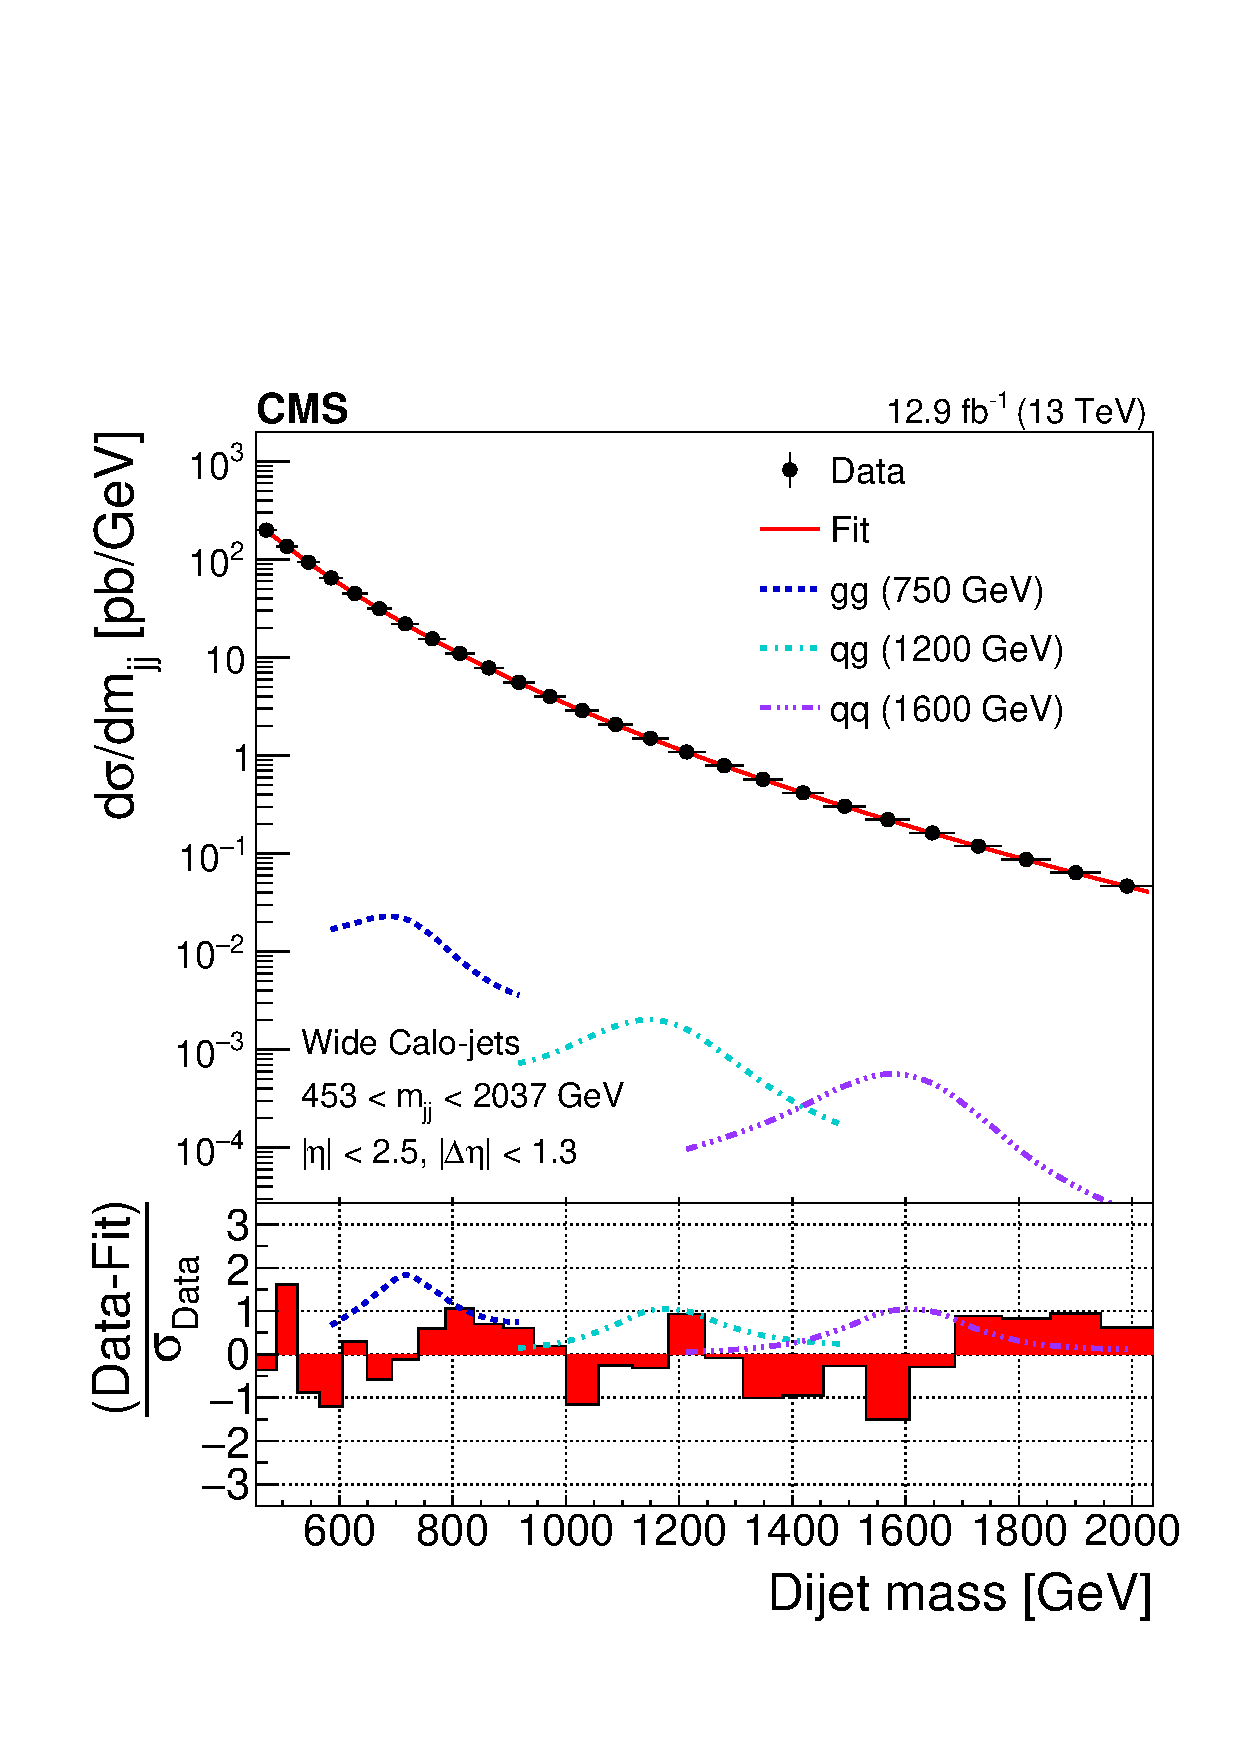
\includegraphics[width=0.48\textwidth]{figs/dijet/fit_mjj_Full_CaloDijet2016.pdf}
    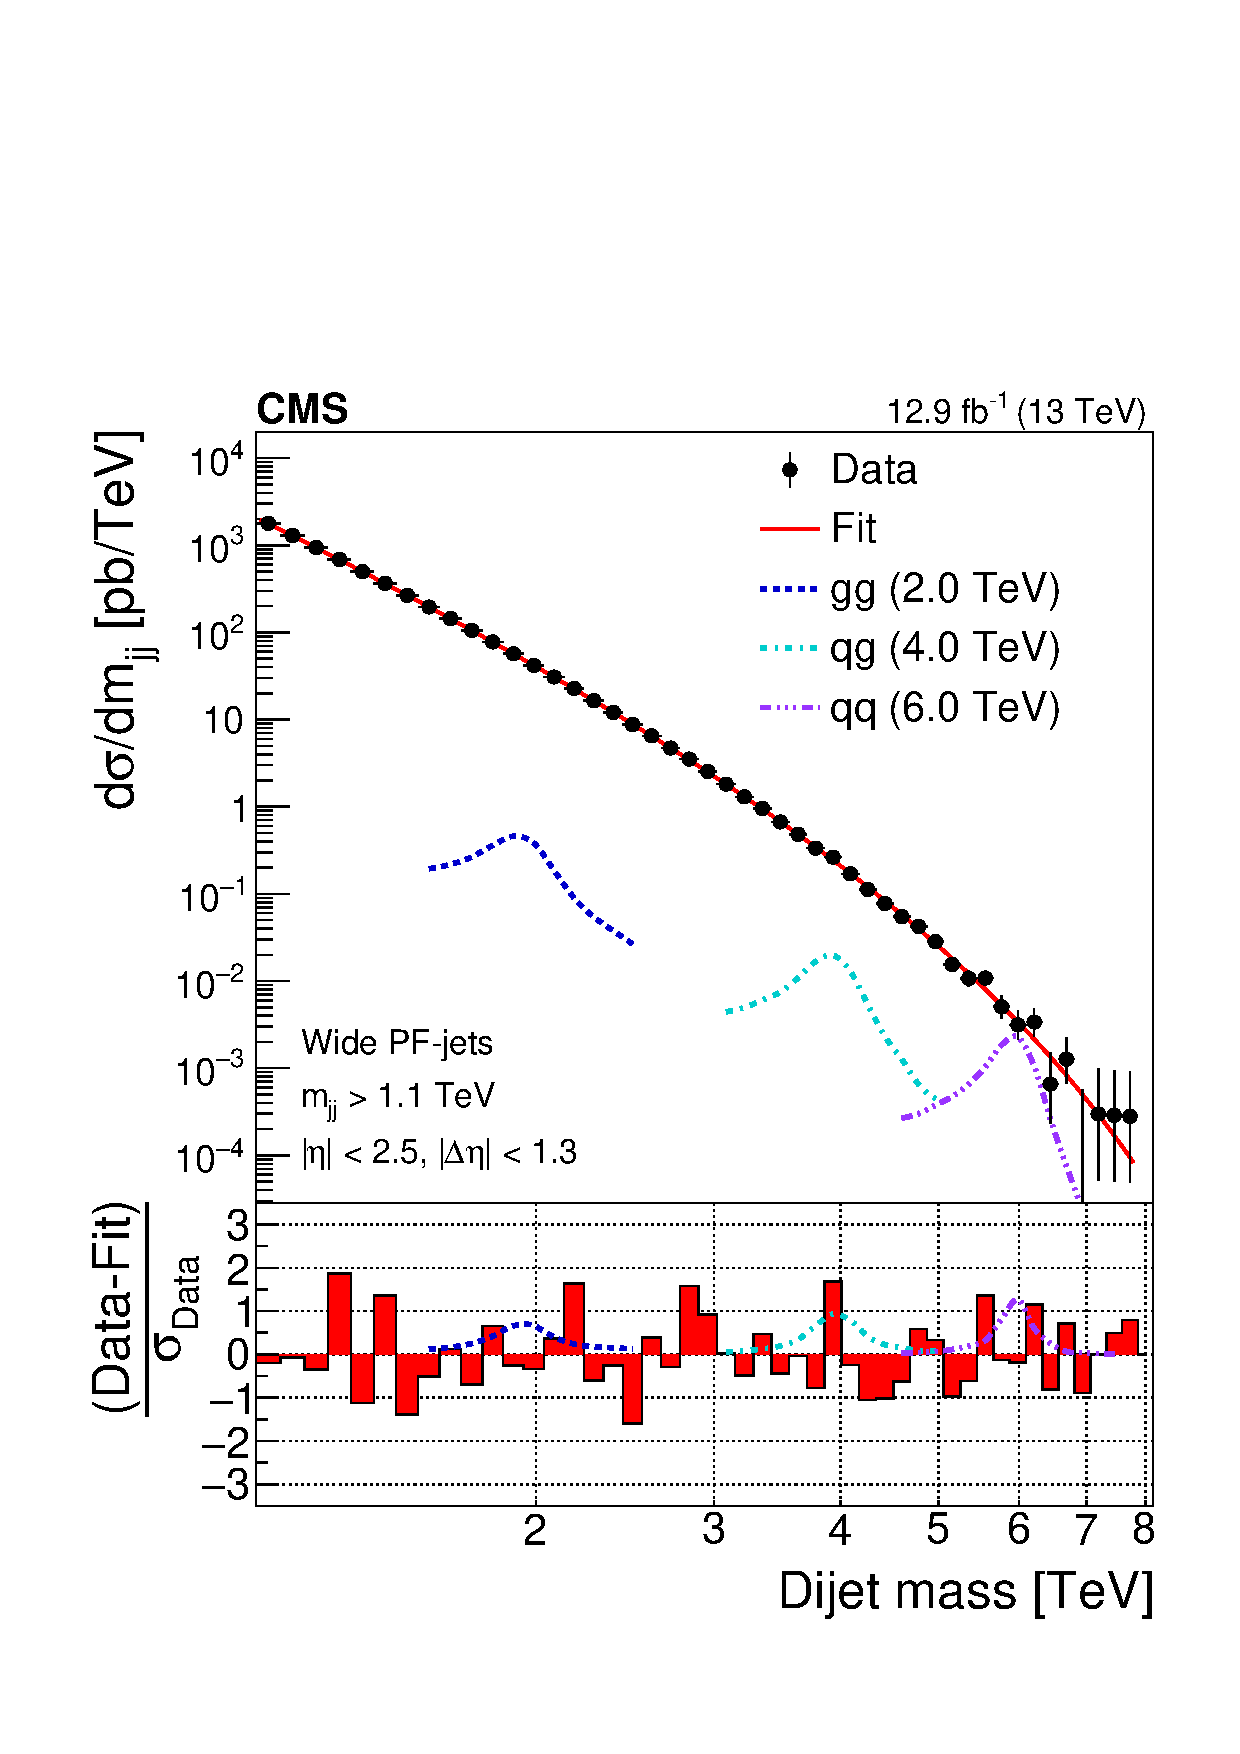
\includegraphics[width=0.48\textwidth]{figs/dijet/fit_mjj_Full_PFDijet2016.pdf}
   \caption{
    Dijet mass spectrum (points) compared to a fitted
  parameterization of the background (solid curve) for the low-mass search (left) and 
  the high-mass search (right).
  The lower panel in each plot shows the difference between the data and the
  fitted parametrization, divided by the statistical uncertainty of the data. Predicted 
  signals from narrow gluon-gluon, quark-gluon, and quark-quark resonances are shown with cross section 
  equal to the observed upper limit at 95\% CL.}
    \label{figDataAndFit}
  \end{center}
\end{figure}


Fig.~\ref{figDataAndFit} shows
the dijet mass spectra, defined as the observed number of events in each bin divided by the
integrated luminosity and bin width, with predefined bins of width corresponding to the
dijet mass resolution~\cite{Khachatryan:2010jd}. 
The highest mass event has a dijet mass of \highestMass and is shown in Fig.~\ref{figEvent}. 
\begin{figure}[hbtp]
  \begin{center}
    \fbox{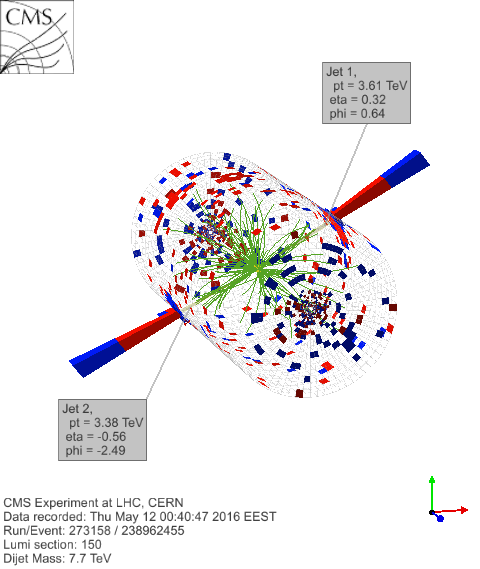
\includegraphics[width=0.5\cmsFigWidth]{figs/dijet/HighMass_event_3d_tower.png}}
    \fbox{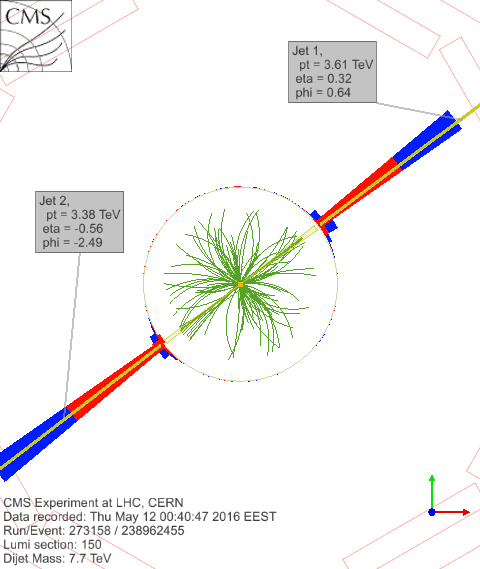
\includegraphics[width=0.5\cmsFigWidth]{figs/dijet/HighMass_event_rho_phi.png}}
    \caption{The event with the highest dijet invariant mass: three dimensional view (left), 2D view in the ($\rho$,$\phi$)
    plane (right). The \pt, $\eta$, and $\phi$ values of the two
    wide jets are indicated. The invariant mass of the two wide jets is \highestMass.}
    \label{figEvent}
  \end{center}
\end{figure}
The dijet mass spectra for the high-mass search
and for the low-mass search are fit with the 
following parameterization:
\begin{equation} 
\frac{{\rd}\sigma}{{\rd}\mjj} =
\frac{p_{0} (1 - x)^{p_{1}}}{x^{p_{2} + p_{3} \log{(x)}}}\ ,
\label{eqBackgroundParam}
\end{equation}
where $x=\mbox{\mjj}/\sqrt{s}$ and $p_0$, $p_1$, $p_2$, and $p_3$ are four fitted parameters.
The functional form in Eqn.~\ref{eqBackgroundParam} was also used in previous
searches~\cite{Khachatryan:2016ecr,Khachatryan:2015dcf,Khachatryan:2010jd,Chatrchyan2011123,CMS:2012yf,Chatrchyan:2013qhXX,Khachatryan:2015sja,
ATLAS:2015nsi,ATLAS2010,Aad:2011aj,Aad201237,ATLAS:2012pu,Aad:2014aqa,refCDFrun2} to describe the data. 
In Fig.~\ref{figDataAndFit} we show the result of binned maximum likelihood fits, which yields the following chi-squared per number 
of degrees of freedom: $\chi^2/\mathrm{NDF}=33.3/42$ for the high-mass search, $\chi^2/\mathrm{NDF}=17.3/22$ for the low-mass search.  
The dijet mass spectra are well modeled by the background fits.  In the lower panels of Fig.~\ref{figDataAndFit}, in the region of dijet mass between 1.1 and 2 \TeV, 
the bin-by-bin differences between the data and the background fit are not identical in the two searches 
because fluctuations in reconstructed dijet mass for Calo jets and PF jets are not completely correlated.

\section{Search}

We search in the dijet mass spectrum for narrow resonances. 
Fig.~\ref{figMassShapes} shows examples of dijet mass distributions 
for simulated signal events  
generated with the \PYTHIA8~\cite{Sjostrand:2007gs} program.
\begin{figure}[hbtp]
  \begin{center}
     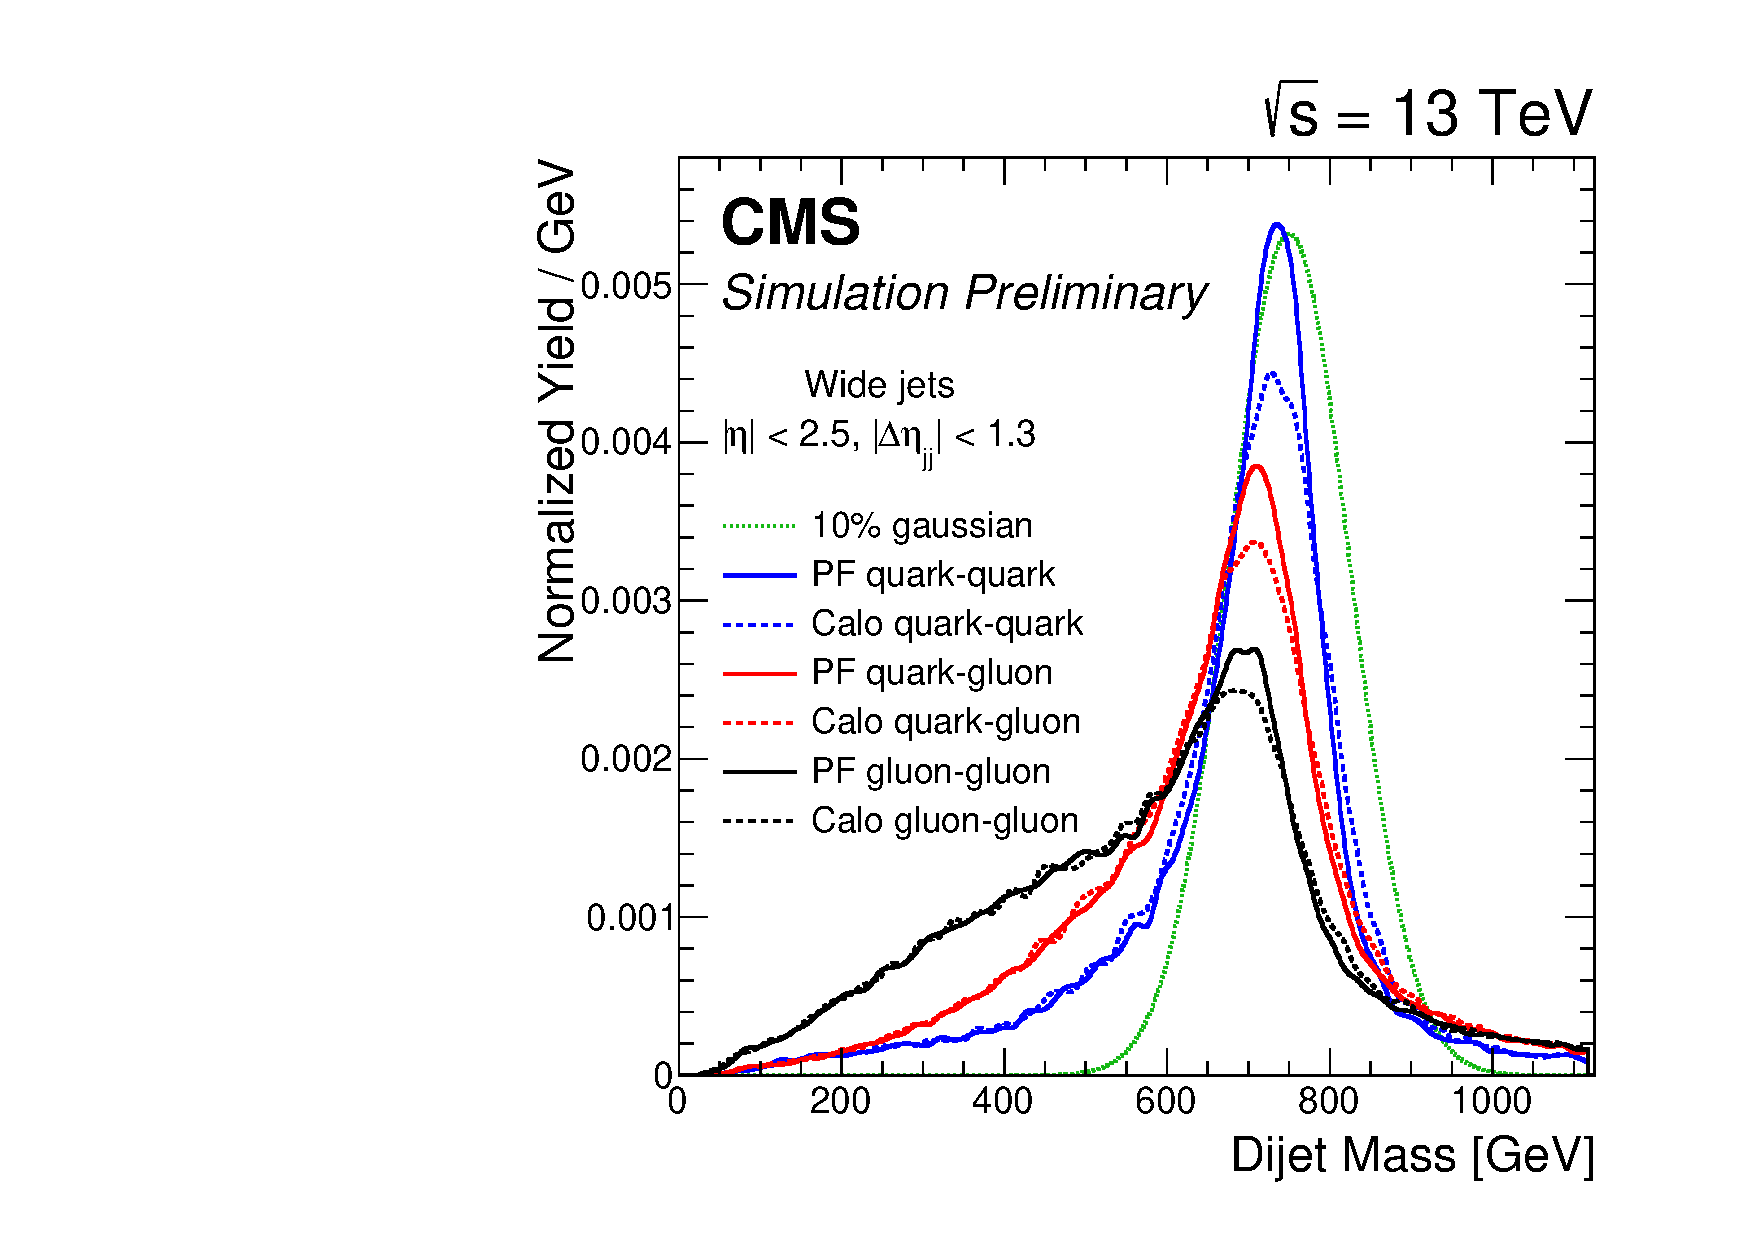
\includegraphics[width=0.48\textwidth]{figs/dijet/signal_shapes_M-750.pdf}
      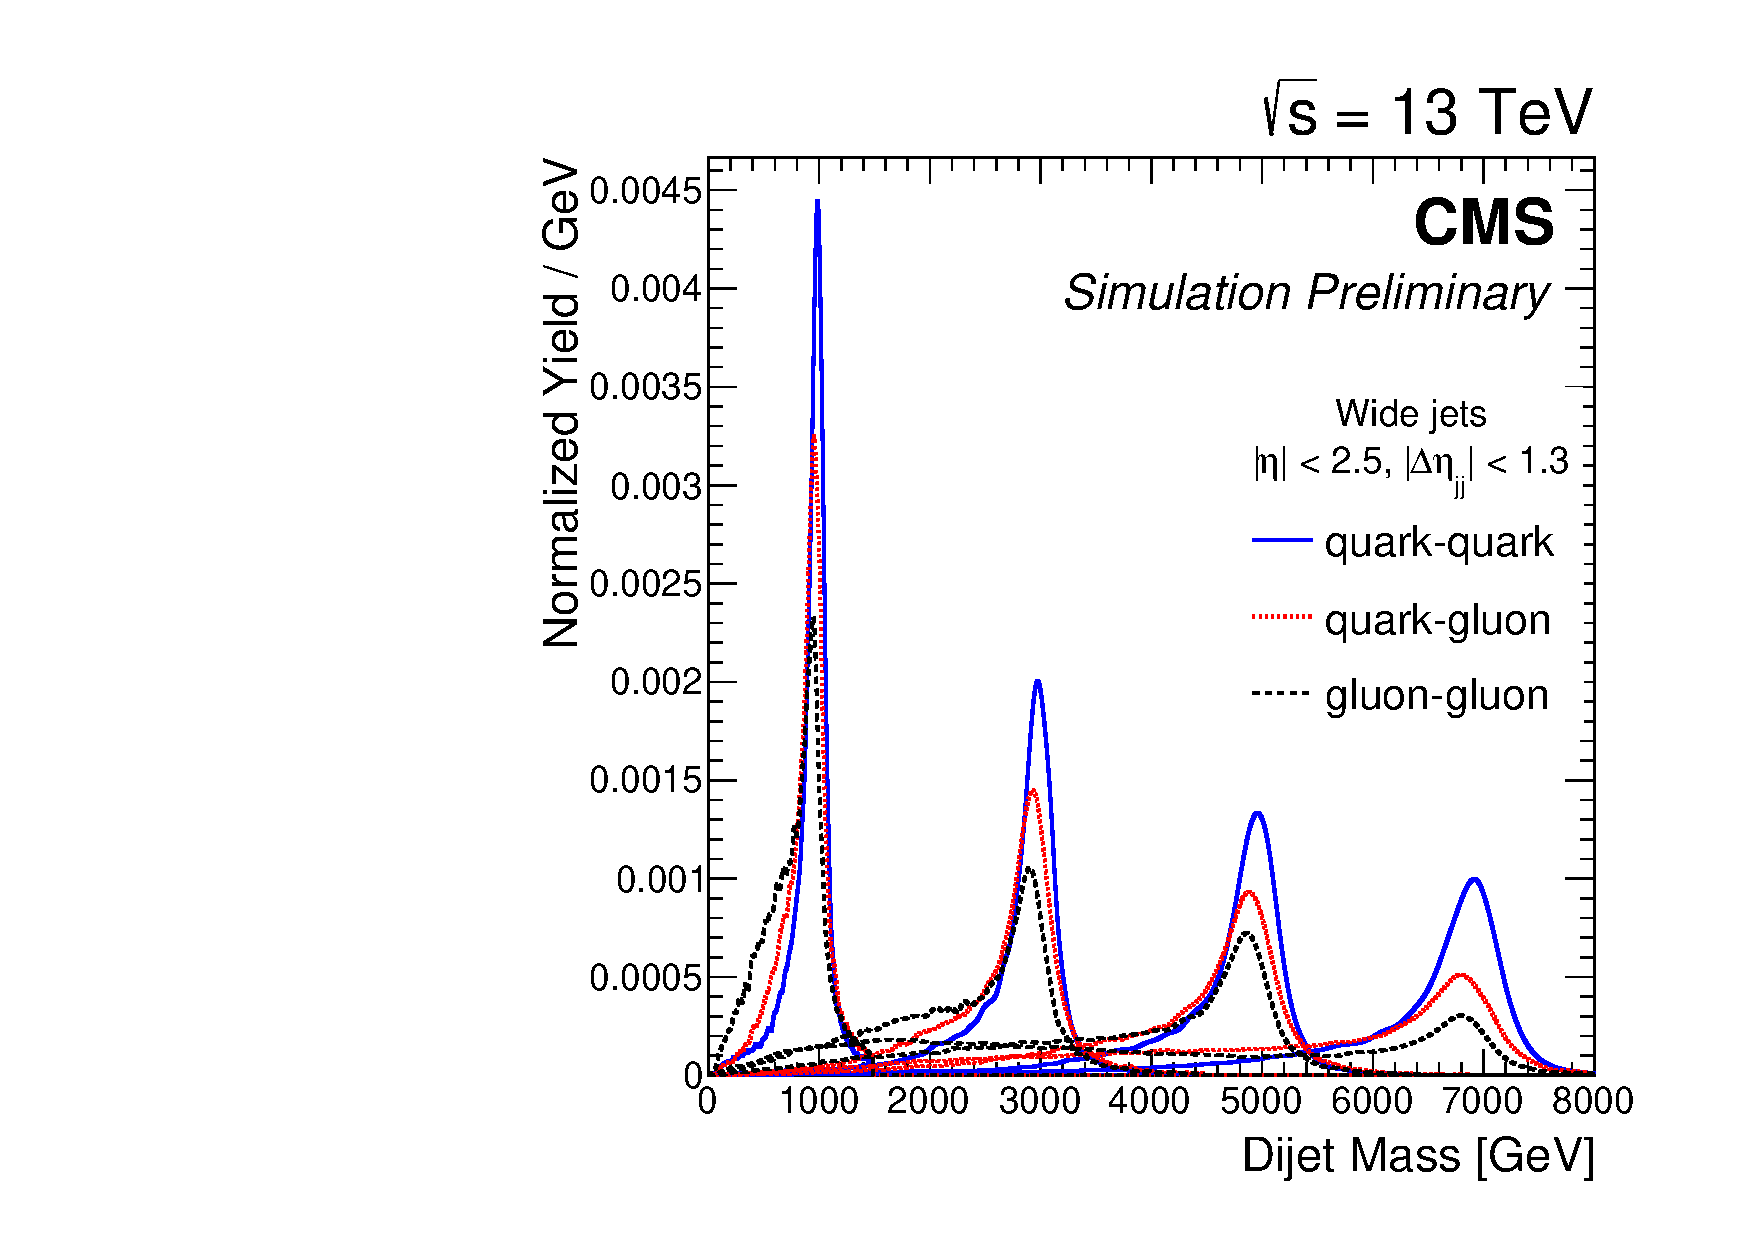
\includegraphics[width=0.48\textwidth]{figs/dijet/signal_shapes_high_mass.pdf}
  \caption{
   The reconstructed resonance mass spectrum predicted by
  the {\PYTHIA8} MC event generator including
  simulation of the detector. Resonances from quark-quark processes modeled by $\PQq\PAQq\to \PXXG \to \PQq\PAQq$  (blue),
quark-gluon processes modeled by $\PQq\Pg\to \Qstar \to \PQq\Pg$ (red),
and gluon-gluon processes modeled by $\Pg\Pg\to \PXXG \to \Pg\Pg$ (black), where \PXXG is an RS graviton
and \Qstar is an excited quark. (left) Resonances generated with a
mass of 750 \GeV are shown for wide jets from PF jet reconstruction (solid) and 
Calo jet reconstruction (dashed). Also shown is a hypothetical Gaussian shape (dotted green) with a mean mass of 750 \GeV and an RMS width equal 
to 10\% of the mean mass.
(right) Resonances generated with a mass of 1, 3, 5, and 7 TeV are shown for wide jets from PF jet reconstruction.}
    \label{figMassShapes}
  \end{center}
\end{figure}
The predicted mass distributions have Gaussian cores from the jet energy resolution,
and tails towards lower mass values primarily from QCD radiation. The
contribution of this low-mass tail to the lineshape depends on the
parton content of the resonance ($\PQq\PQq$, $\PQq\Pg$, or $\Pg\Pg$).  Resonances
containing gluons, which emit QCD radiation more strongly than
quarks, have a more pronounced tail.  In Fig.~\ref{figMassShapes}, for a resonance mass of 750 \GeV, we also show
a hypothetical Gaussian shape with an RMS width of 10\%, which is one of the widths used by the ATLAS 
experiment for their generic limits on Gaussian resonances. Fitting the core of the CMS $\PQq\PQq$ resonance lineshape
for Calo jets to a truncated Gaussian also gives an RMS width of approximately 10\% at the resonance mass value 
of 750 GeV. Note that the expected distributions
of dijet resonances from PYTHIA differ from a Gaussian shape centered at the 
resonance mass. This is primarily because of QCD radiation which produces significant tails and
shifts the peak to a lower value of dijet mass.  These real physical effects in the PYTHIA resonance shapes
result in lower search sensitivity compared to hypothetical Gaussian shapes which neglect these
effects. 

Fig.~\ref{figDataAndFit} includes the signal distributions of quark-quark, quark-gluon and gluon-gluon 
resonances with signal cross sections excluded at 95\% CL by this analysis, as described below.
There is no evidence for a narrow resonance in the data, as seen in Fig.~\ref{figDataAndFit}.
The most significant excess in the data relative to the background fit occurs in the low-mass search
around 800 GeV in dijet mass. Fitting this data to a gluon-gluon resonance with a mass of 850 \GeV 
yields a significance of 2.6 standard deviations.
%The significance from a fit to a resonance with mass 750 GeV is XX for a $\Pg\Pg$ resonance
%and YY standard deviations for a $\Pq\Pq$ resonance.  


\section{Model-independent interpretation}

We use the dijet mass spectrum from wide jets, the background 
parameterization, and the dijet resonance shapes to set
limits on new particles decaying to the parton pairs $\PQq\PQq$ (or $\PQq\PAQq$), $\Pq\Pg$, and $\Pg\Pg$. A separate limit is determined
for each final state ($\PQq\PQq$, $\Pq\Pg$ and $\Pg\Pg$) because of the dependence of the
dijet resonance shape on the type of the two final-state partons.

The dominant sources of systematic uncertainty are the jet energy scale, jet energy resolution,
integrated luminosity, and the estimation of background. The uncertainty in the jet energy scale is \jecUncert,
determined from Run 2 data using the methods described in Ref.~\cite{Chatrchyan:2011ds}.
This uncertainty is propagated to the limits by shifting the dijet mass shape for signal by $\pm$\jecUncert.
The uncertainty in the jet energy
resolution translates into an uncertainty of 10\% in the resolution of the dijet
mass~\cite{Chatrchyan:2011ds}, and is propagated to the limits by increasing and decreasing by 10\% the reconstructed
width of the dijet mass shape for signal.
The uncertainty in the
integrated luminosity is \lumiUncert, and is propagated to the normalization of
the signal.
Changes in the values of the parameters describing the background introduce a change in the signal strength
that is accounted for as a systematic uncertainty.


The modified frequentist method~\cite{Junk1999,bib-cls} is
utilized to set upper limits on signal cross sections, following the prescription
described in Ref.~\cite{LHCCLs} and Sec.~\ref{sec:limit8TeV} of this thesis.  We use a multi-bin counting experiment likelihood, which is
a product of Poisson distributions corresponding to different bins.
We evaluate the likelihood independently at each value of resonance pole mass from 600\GeV to 1600\GeV in 50\GeV 
steps in the low-mass search, and from 1.6\TeV to 7.5\TeV in 100\GeV steps in the high-mass search. 
Gaussian distributions are used to model systematic uncertainties in the jet energy scale and jet energy
resolution, and log normal distributions are used to model uncertainties in the integrated luminosity, treated as nuisance 
parameters within a constraint placed on the likelihood. For this methodology, the 
systematic uncertainty on the background is automatically evaluated via profiling, effectively 
refitting for the optimal values of the background parameters for each value of resonance cross section.
The procedure gave the same limits as the Bayesian procedure used previously for dijet resonance
searches at CMS~\cite{Khachatryan:2015sja}. For both the Bayesian and modified frequentist statistical procedures 
we find that the background systematic uncertainty has the largest effect on the limit. The amount the
background uncertainty affects the limit depends significantly on the signal shape and the resonance mass, with the largest effect for
the gluon-gluon resonances and the smallest effect for the hypothetical Gaussian resonances in the low-mass search,
and the effect decreases as the resonance mass increases. %The affect of systematics can be seen in the lower panels of 
%Fig.~\ref{figDataAndFit}, where, for example, the excluded $\Pg\Pg$ resonance signal at 750 \GeV is more significantly above the data than 
%is the excluded $\PQq\PQq$ resonance signal at 6 \TeV.


%Signal injection and extraction tests with pseudo-data confirmed that the chosen
%background function does not bias the extraction of a potential signal.
%Alternate background functions were tried, and Eq.~\ref{eqBackgroundParam} was the 
%only function with four our fewer parameters that fit our measured data in the low mass search.  

%We performed signal injection and extraction tests with two background parameterization choices.
%First we generated pseudo-data for signals, with the background from Eq.~\ref{eqBackgroundParam}, and verified 
%that the signal cross sections extracted were the same as those generated. Then we found another background parameterization 
%which fit the measured collision data,
% ${\rd}\sigma/\rd\mjj=\exp(\ln{(P_0)} + P_1x^{P_2} + P_3(1-x)^{P_4})$, and we
% used it to generate pseudo-data with signals. Finally, 
%the injected signals were extracted using Eq.~\ref{eqBackgroundParam} to fit the background, and the resulting change in the signal cross 
%sections were negligible.

The potential bias introduced through the choice of background parameterization 
was investigated using signal injection and extraction tests with two
background parameterization choices. First, we generated pseudo-data
with injected signal of strength $\mu$ using an alternative background
parameterization
\begin{equation}
\frac{\rd\sigma}{\rd\mjj}=p_0e^{p_1[x^{p_2} + (1-x)^{p_3}]}~.
\ref{eqn:modexp}
\end{equation}
Then, we fit these data with the nominal background parameterization
of Eqn.~\ref{eqBackgroundParam} in order to extract the measured
signal strength $\hat{\mu}$ and its uncertainty $\sigma_{\mu}$. The resulting bias $(\mu-\hat{\mu})/\sigma_{\mu}$
was found to be negligible.

\begin{figure*}[hbtp]
  \centering
    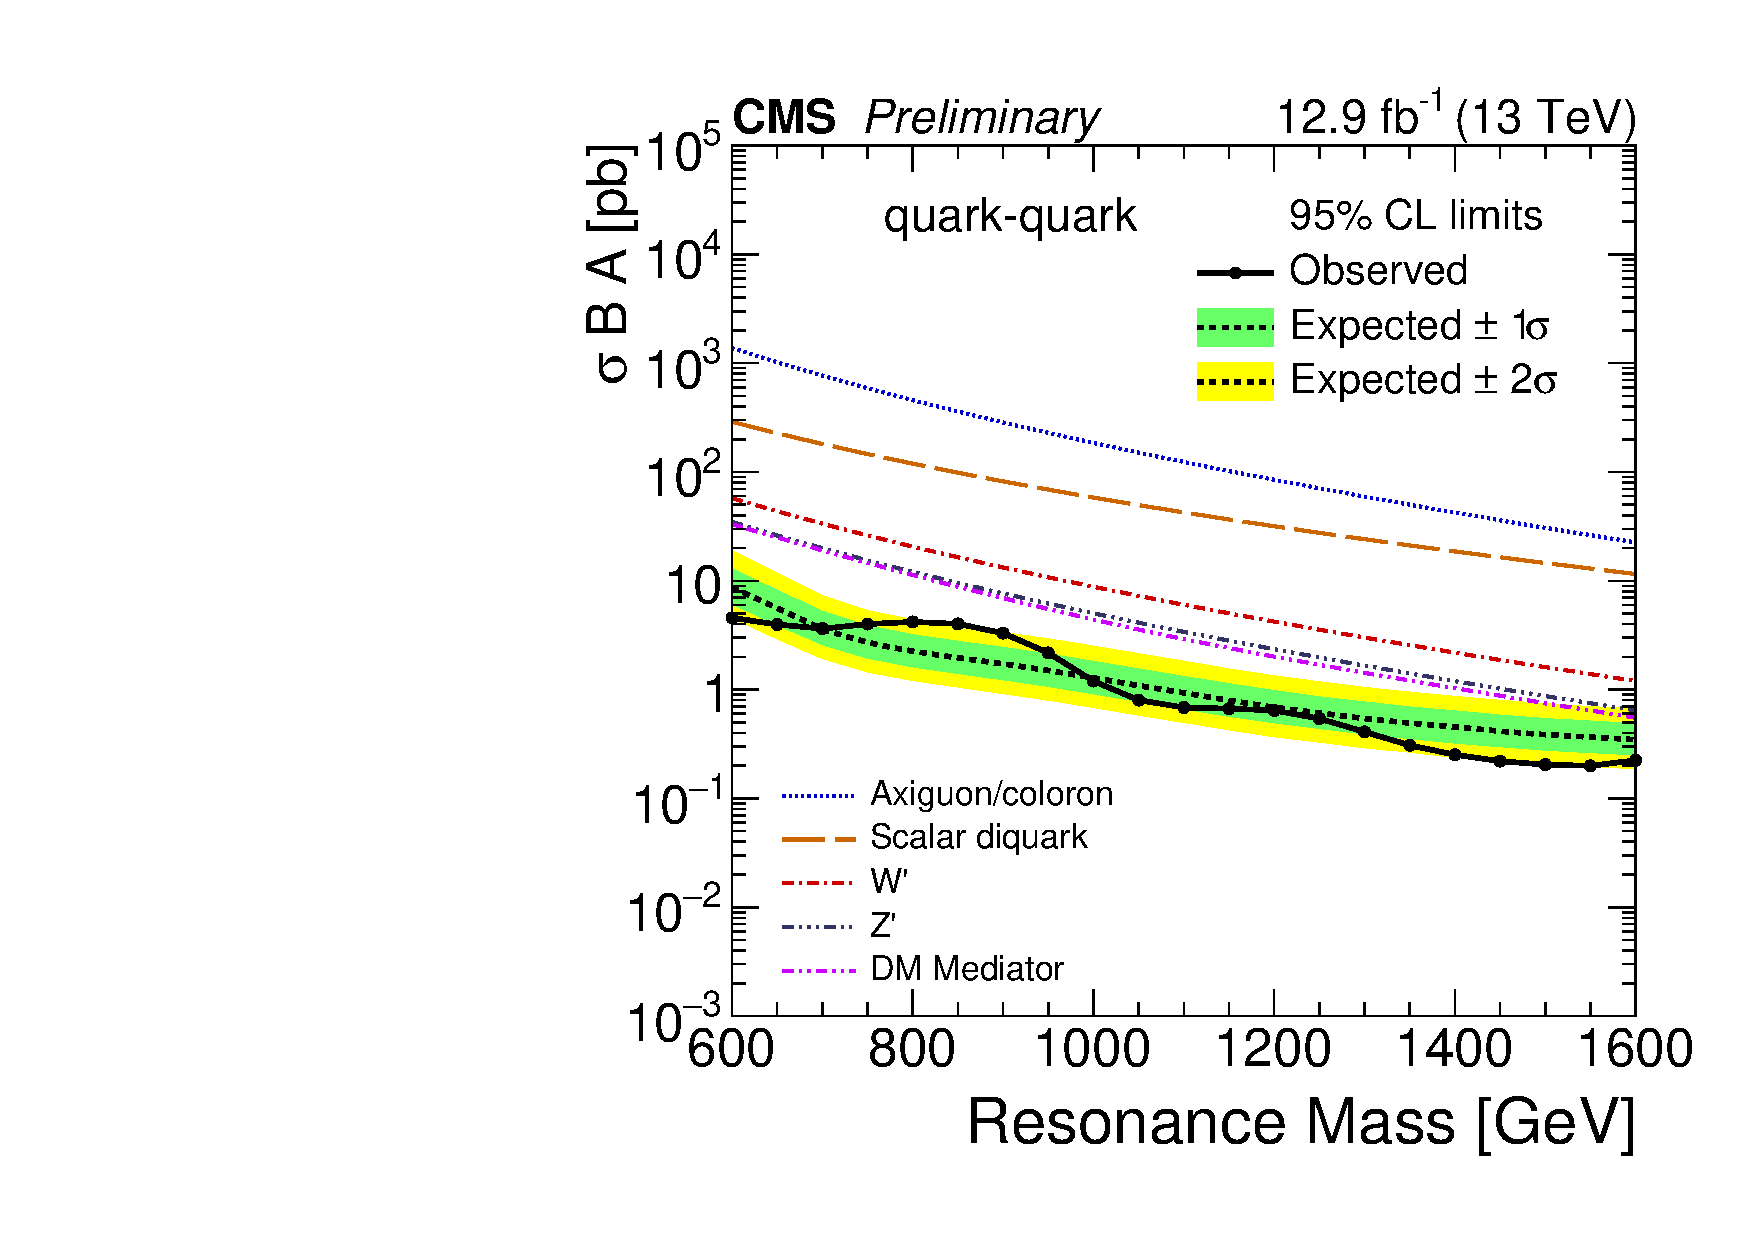
\includegraphics[width=0.48\textwidth]{figs/dijet/limits_freq_qq_calodijet2016.pdf}
    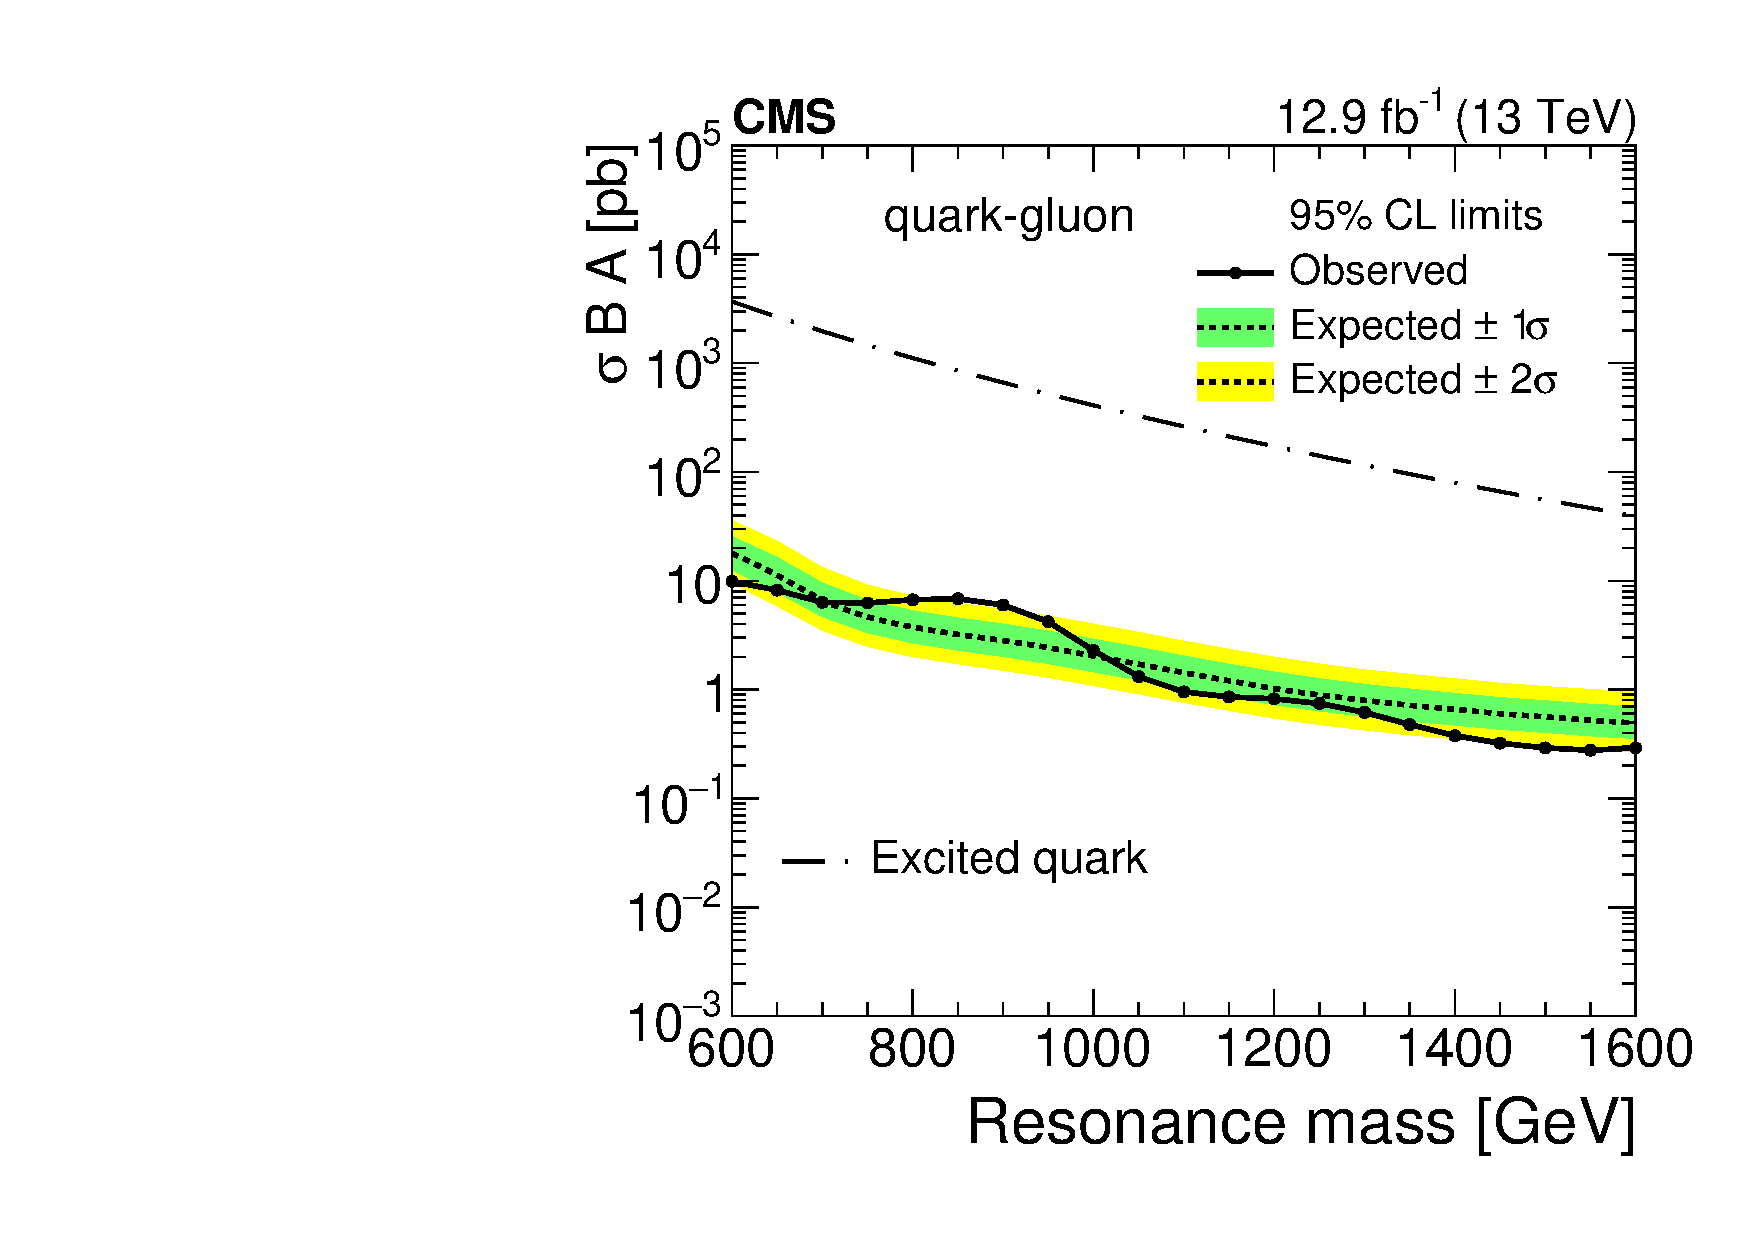
\includegraphics[width=0.48\textwidth]{figs/dijet/limits_freq_qg_calodijet2016.pdf}
    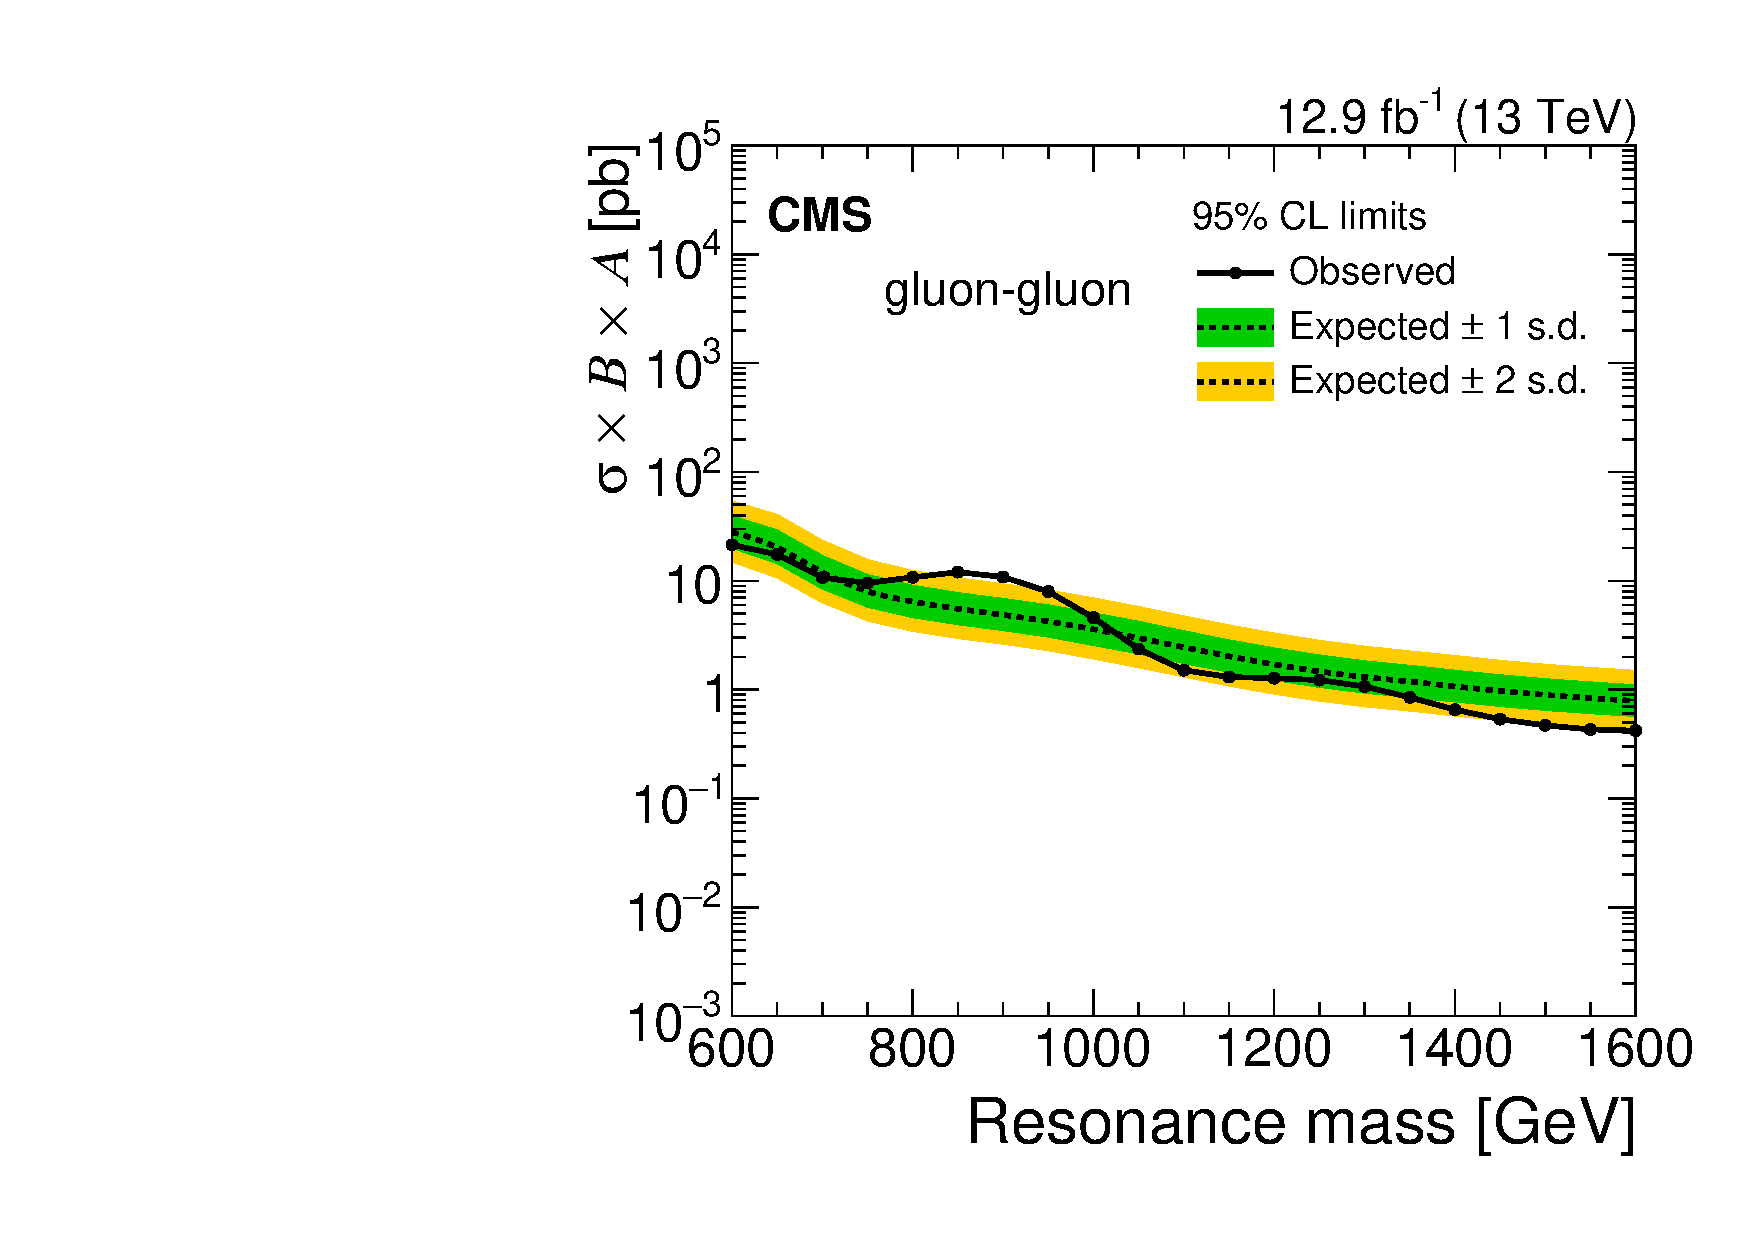
\includegraphics[width=0.48\textwidth]{figs/dijet/limits_freq_gg_calodijet2016.pdf}
    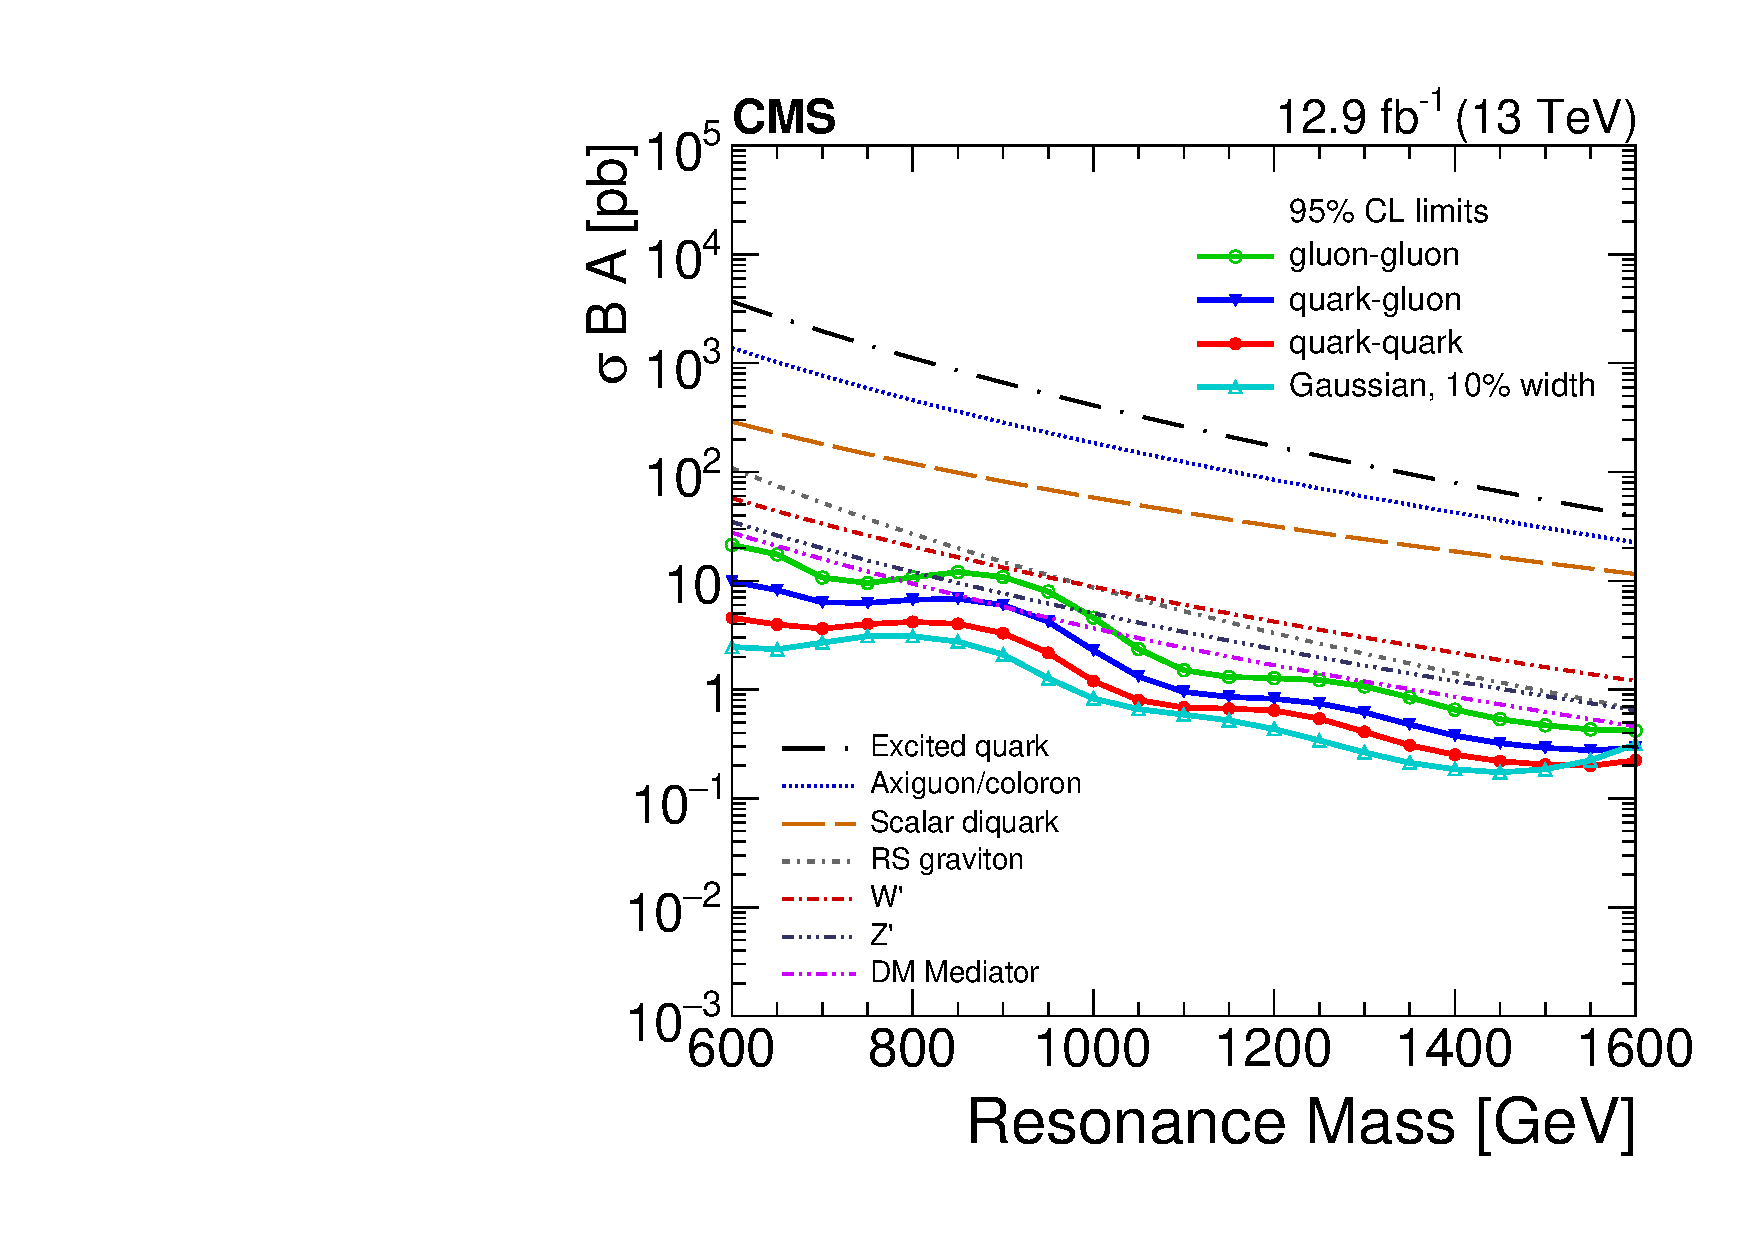
\includegraphics[width=0.48\textwidth]{figs/dijet/limits_freq_gg_qg_qq_gaus10_calodijet2016.pdf}
    \caption{Limits from the low-mass search~\cite{CMS-PAS-EXO-16-032,jmgd}. The observed 95\% \CL upper limits on the product of the cross section, branching fraction, and acceptance for
    quark-quark (top left), quark-gluon (top right), and gluon-gluon (bottom left) type dijet resonances.
    The corresponding expected limits (dashed) and their variation at the 1 and 2 standard deviation levels (shaded bands) are also shown.   
    (bottom right) The observed limits (solid) are summarized for fully simulated shapes from all three physical types of resonances 
    along with the limit for a hypothetical Gaussian shape with RMS width equal to 10\% of the mean mass.
    Limits are compared 
    to the predicted cross sections of  
    excited quarks~\cite{ref_qstar,Baur:1989kv},
    axigluons~\cite{ref_axi}, colorons~\cite{ref_coloron}, scalar
    diquarks~\cite{ref_diquark}, new gauge bosons $\PWpr$ and
    $\PZpr$~\cite{ref_gauge}, a dark matter mediator for
    $m_{\mathrm{DM}}=1\GeV$~\cite{Boveia:2016mrp,Abdallah:2015ter},
    and RS gravitons~\cite{ref_rsg}.}
    \label{figLimitLow}
\end{figure*}

\begin{figure*}[hbtp]
  \centering
    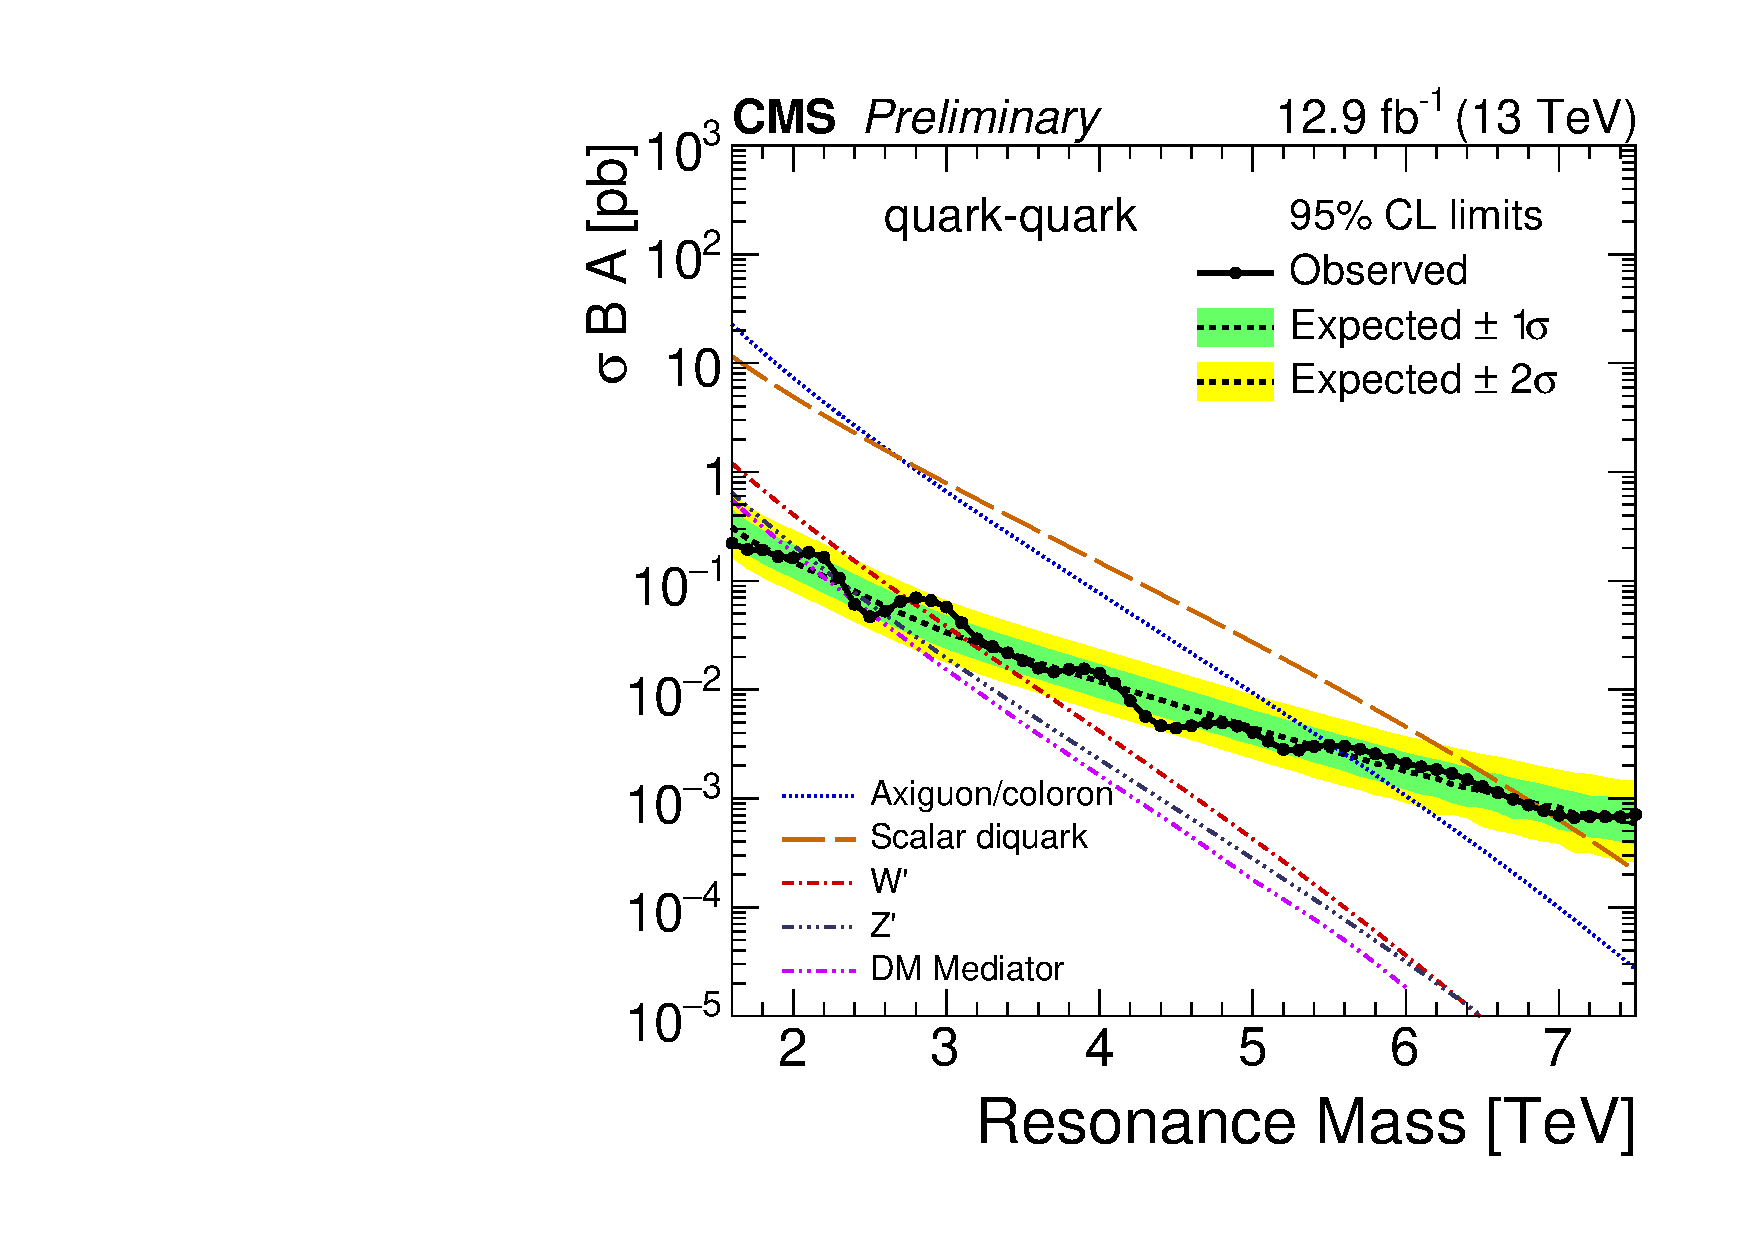
\includegraphics[width=0.48\textwidth]{figs/dijet/limits_freq_qq_pfdijet2016.pdf}
    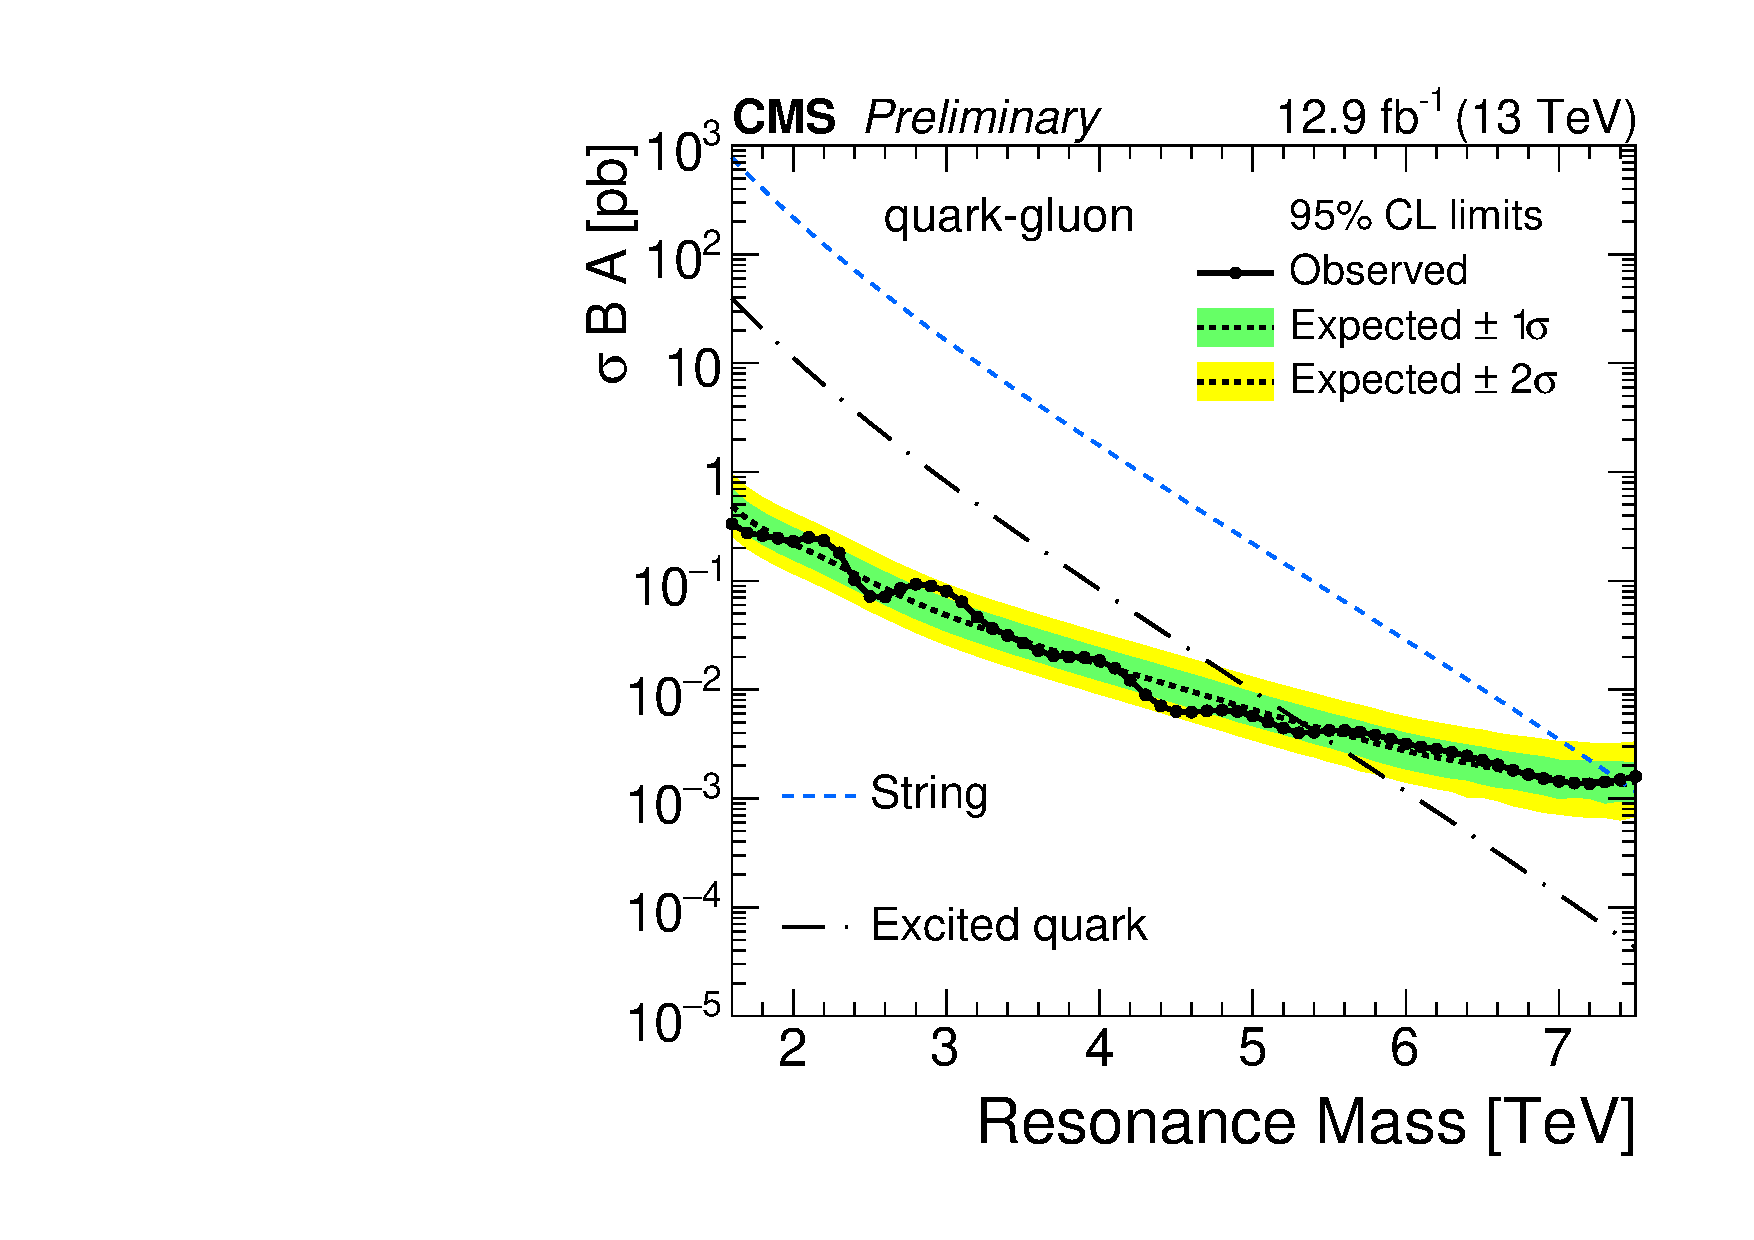
\includegraphics[width=0.48\textwidth]{figs/dijet/limits_freq_qg_pfdijet2016.pdf}
    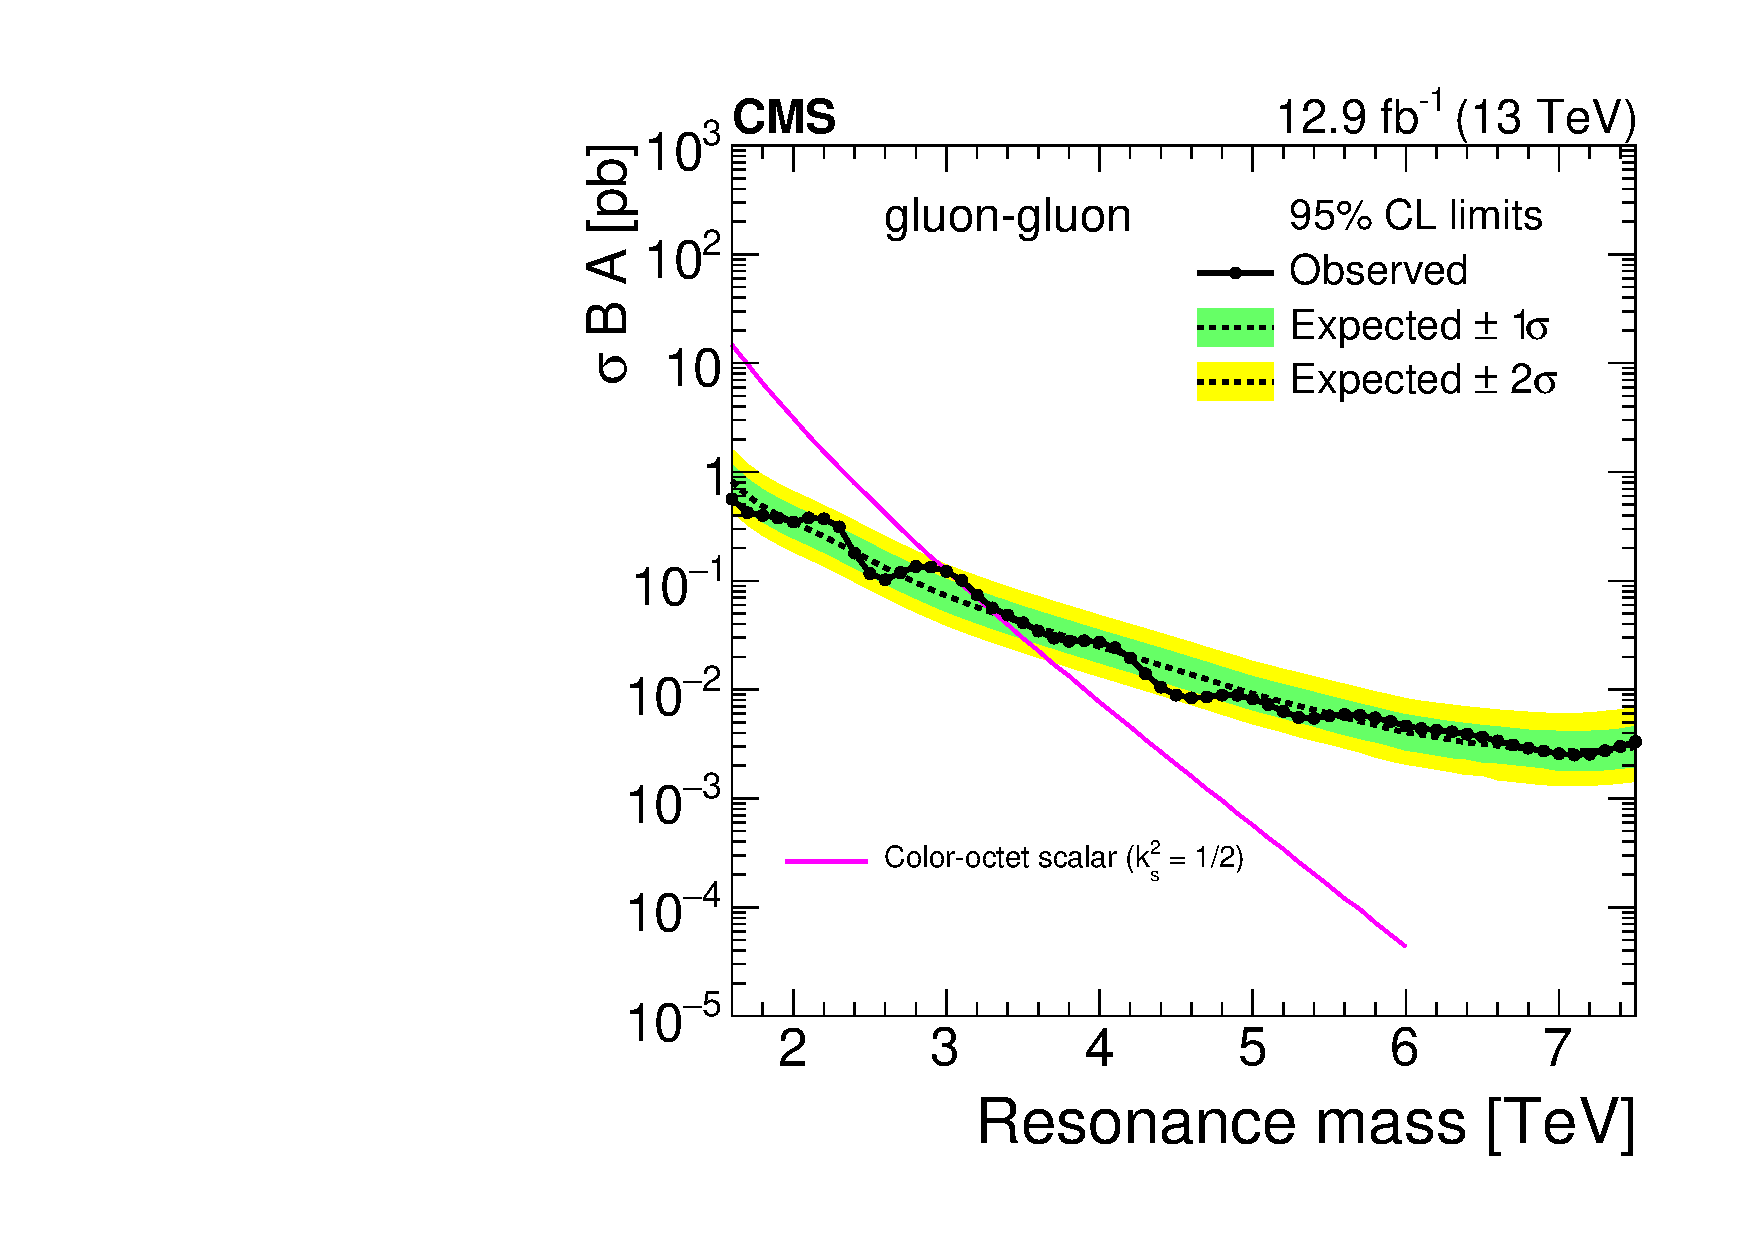
\includegraphics[width=0.48\textwidth]{figs/dijet/limits_freq_gg_pfdijet2016.pdf} 
    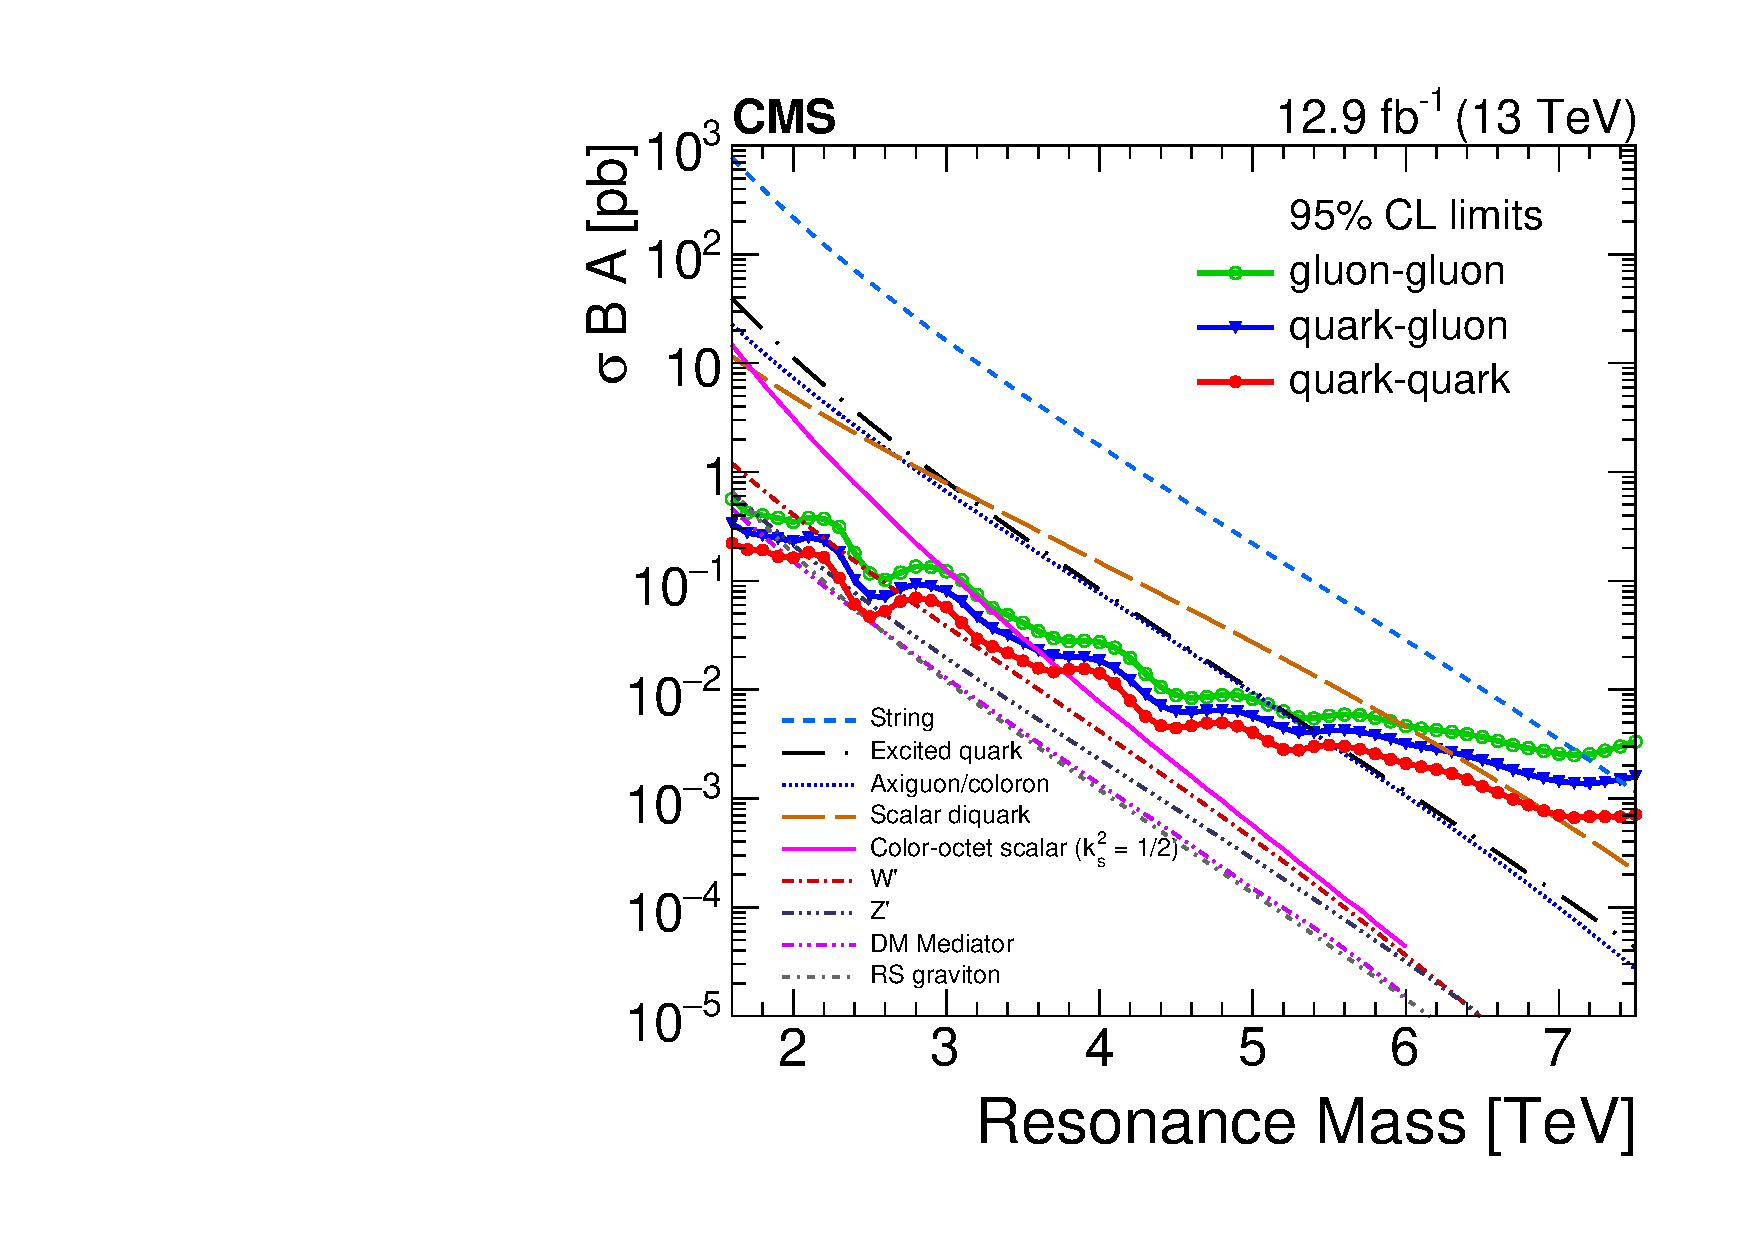
\includegraphics[width=0.48\textwidth]{figs/dijet/limits_freq_gg_qg_qq_pfdijet2016.pdf}
    \caption{Limits from the high-mass search~\cite{CMS-PAS-EXO-16-032,jmgd}. The observed 95\% \CL upper limits on the product of the cross section, branching fraction, and acceptance for
    quark-quark (top left), quark-gluon (top right), and gluon-gluon (bottom left) type dijet resonances.
    The corresponding expected limits (dashed) and their variation 
    at the 1 and 2 standard deviation levels (shaded bands) are also shown.  
    (bottom right) The observed limits (solid) are summarized.  Limits are compared 
    to the predicted cross sections of string resonances~\cite{Anchordoqui:2008di,Cullen:2000ef}, 
    excited quarks~\cite{ref_qstar,Baur:1989kv},
    axigluons~\cite{ref_axi}, colorons~\cite{ref_coloron},  scalar
    diquarks~\cite{ref_diquark}, color-octet
    scalars~\cite{Han:2010rf}, new gauge bosons $\PWpr$ and
    $\PZpr$~\cite{ref_gauge}, a dark matter mediator for
    $m_{\mathrm{DM}}=1\GeV$~\cite{Boveia:2016mrp,Abdallah:2015ter}, and RS gravitons~\cite{ref_rsg}.}
    \label{figLimitHigh}
\end{figure*}

\begin{figure*}[hbtp]
  \centering
    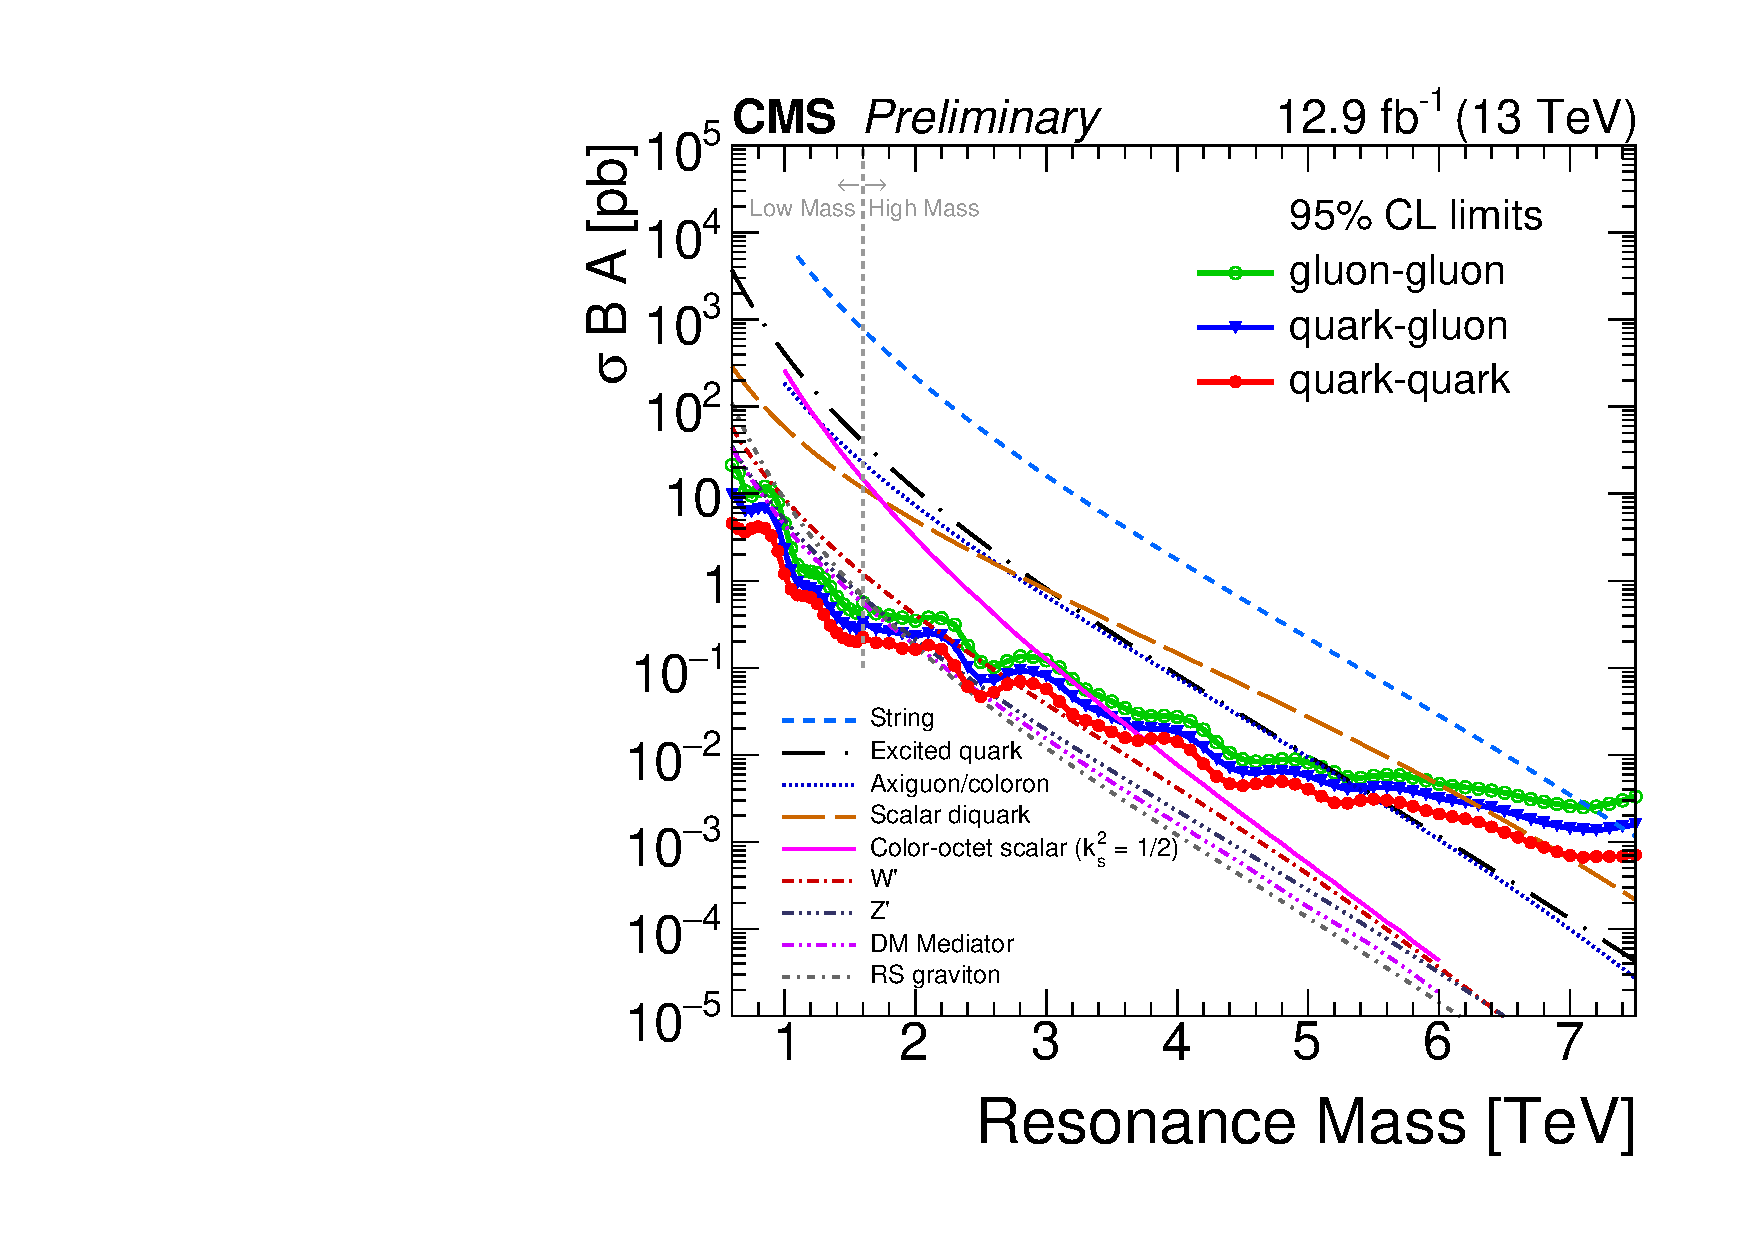
\includegraphics[width=0.9\textwidth]{figs/dijet/limits_freq_gg_qg_qq_calodijet2016_pfdijet2016.pdf}
    \caption{Limits from both the low-mass and high-mass search~\cite{CMS-PAS-EXO-16-032,jmgd}. The observed 95\% \CL upper limits on the product of the cross section, branching fraction, and acceptance for
    quark-quark, quark-gluon, and gluon-gluon type dijet resonances.
    The observed limits (solid) are presented from the low mass search, for resonance masses between \minMassLow and \minMassHigh, and from the high mass search 
    for resonance masses greater than or equal to \minMassHigh. Limits are compared 
    to the predicted cross sections of string resonances~\cite{Anchordoqui:2008di,Cullen:2000ef},  
    excited quarks~\cite{ref_qstar,Baur:1989kv},
    axigluons~\cite{ref_axi}, colorons~\cite{ref_coloron}, scalar
    diquarks~\cite{ref_diquark}, color-octet
    scalars~\cite{Han:2010rf}, new gauge bosons $\PWpr$ and
    $\PZpr$~\cite{ref_gauge}, a dark matter mediator for
    $m_{\mathrm{DM}}=1\GeV$~\cite{Boveia:2016mrp,Abdallah:2015ter}, and RS gravitons~\cite{ref_rsg}.}
    \label{figLimitAll}
\end{figure*}

\begin{figure*}[hbtp]
  \centering
    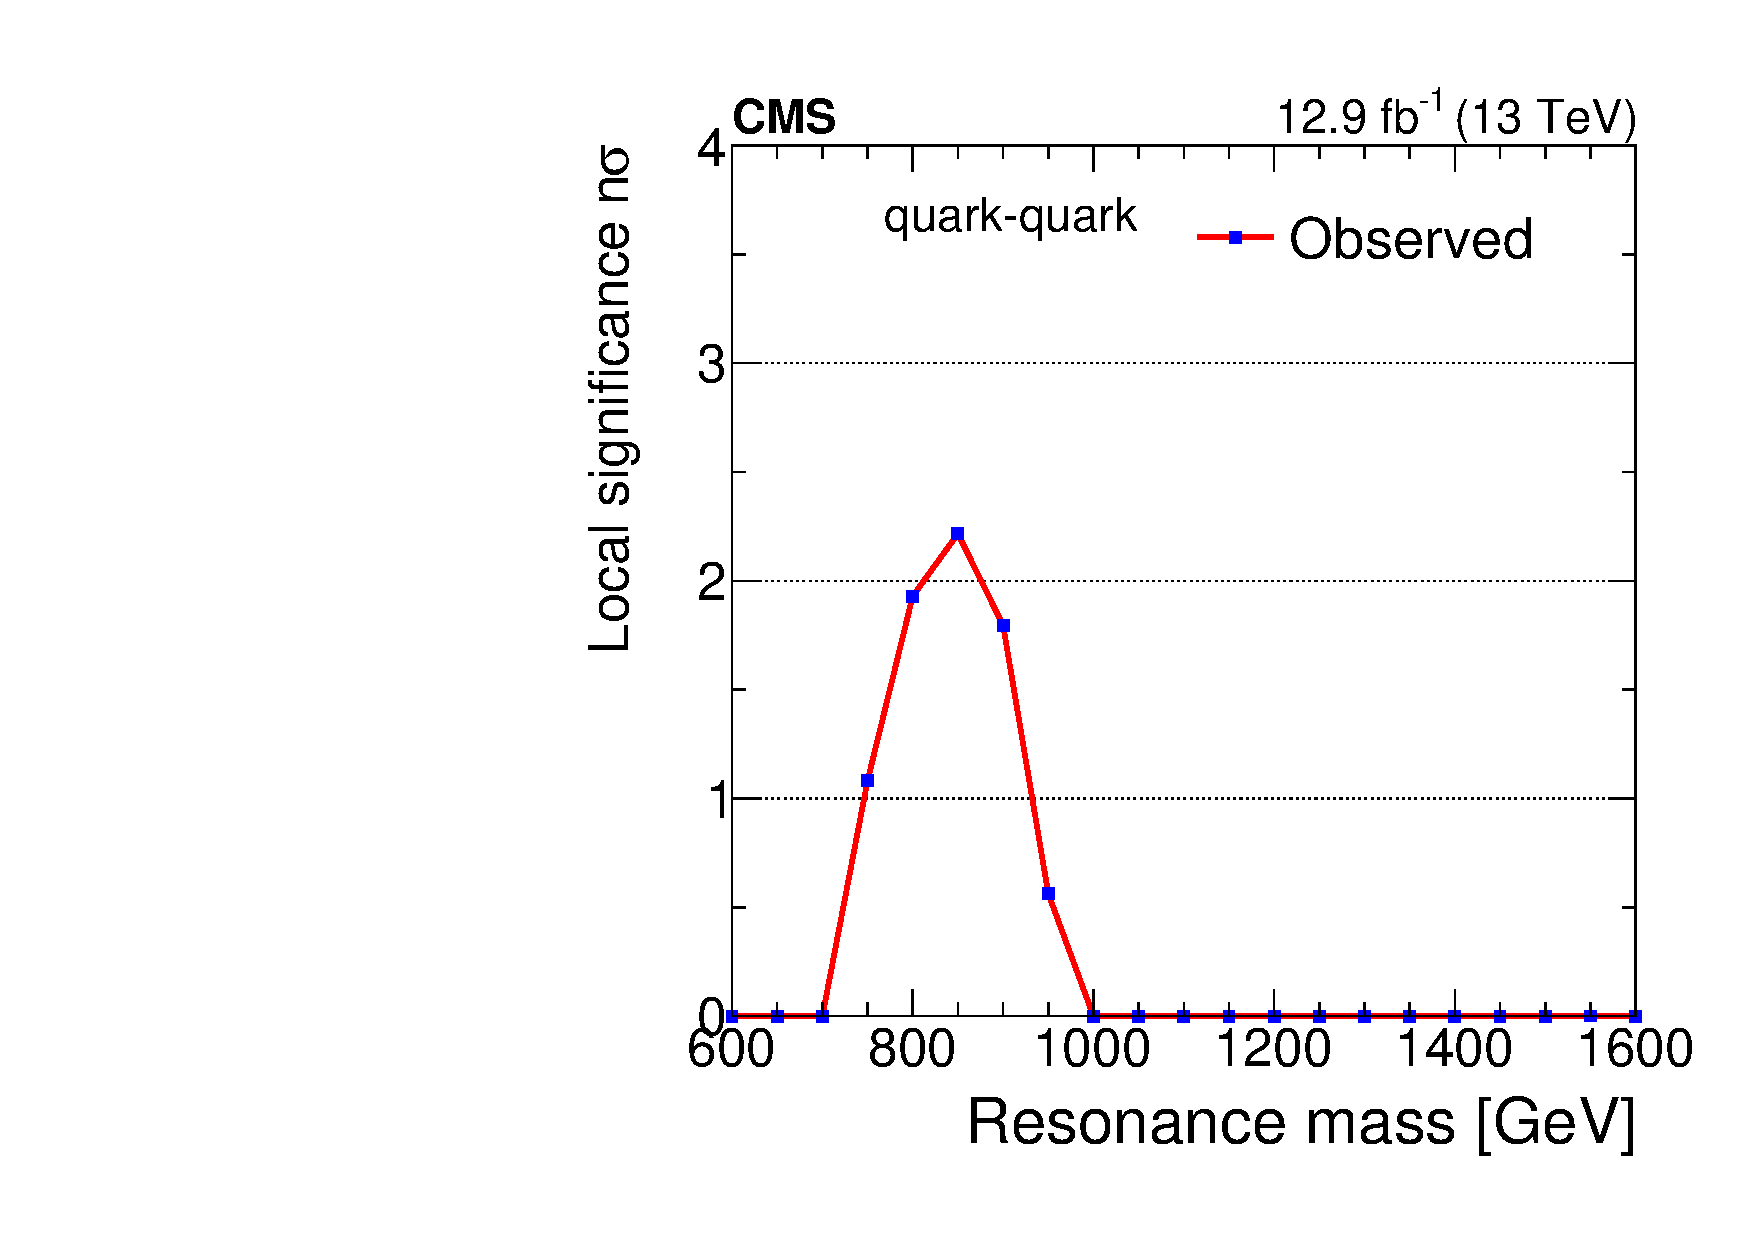
\includegraphics[width=0.48\textwidth]{figs/dijet/signif_qq_calodijet2016.pdf}
    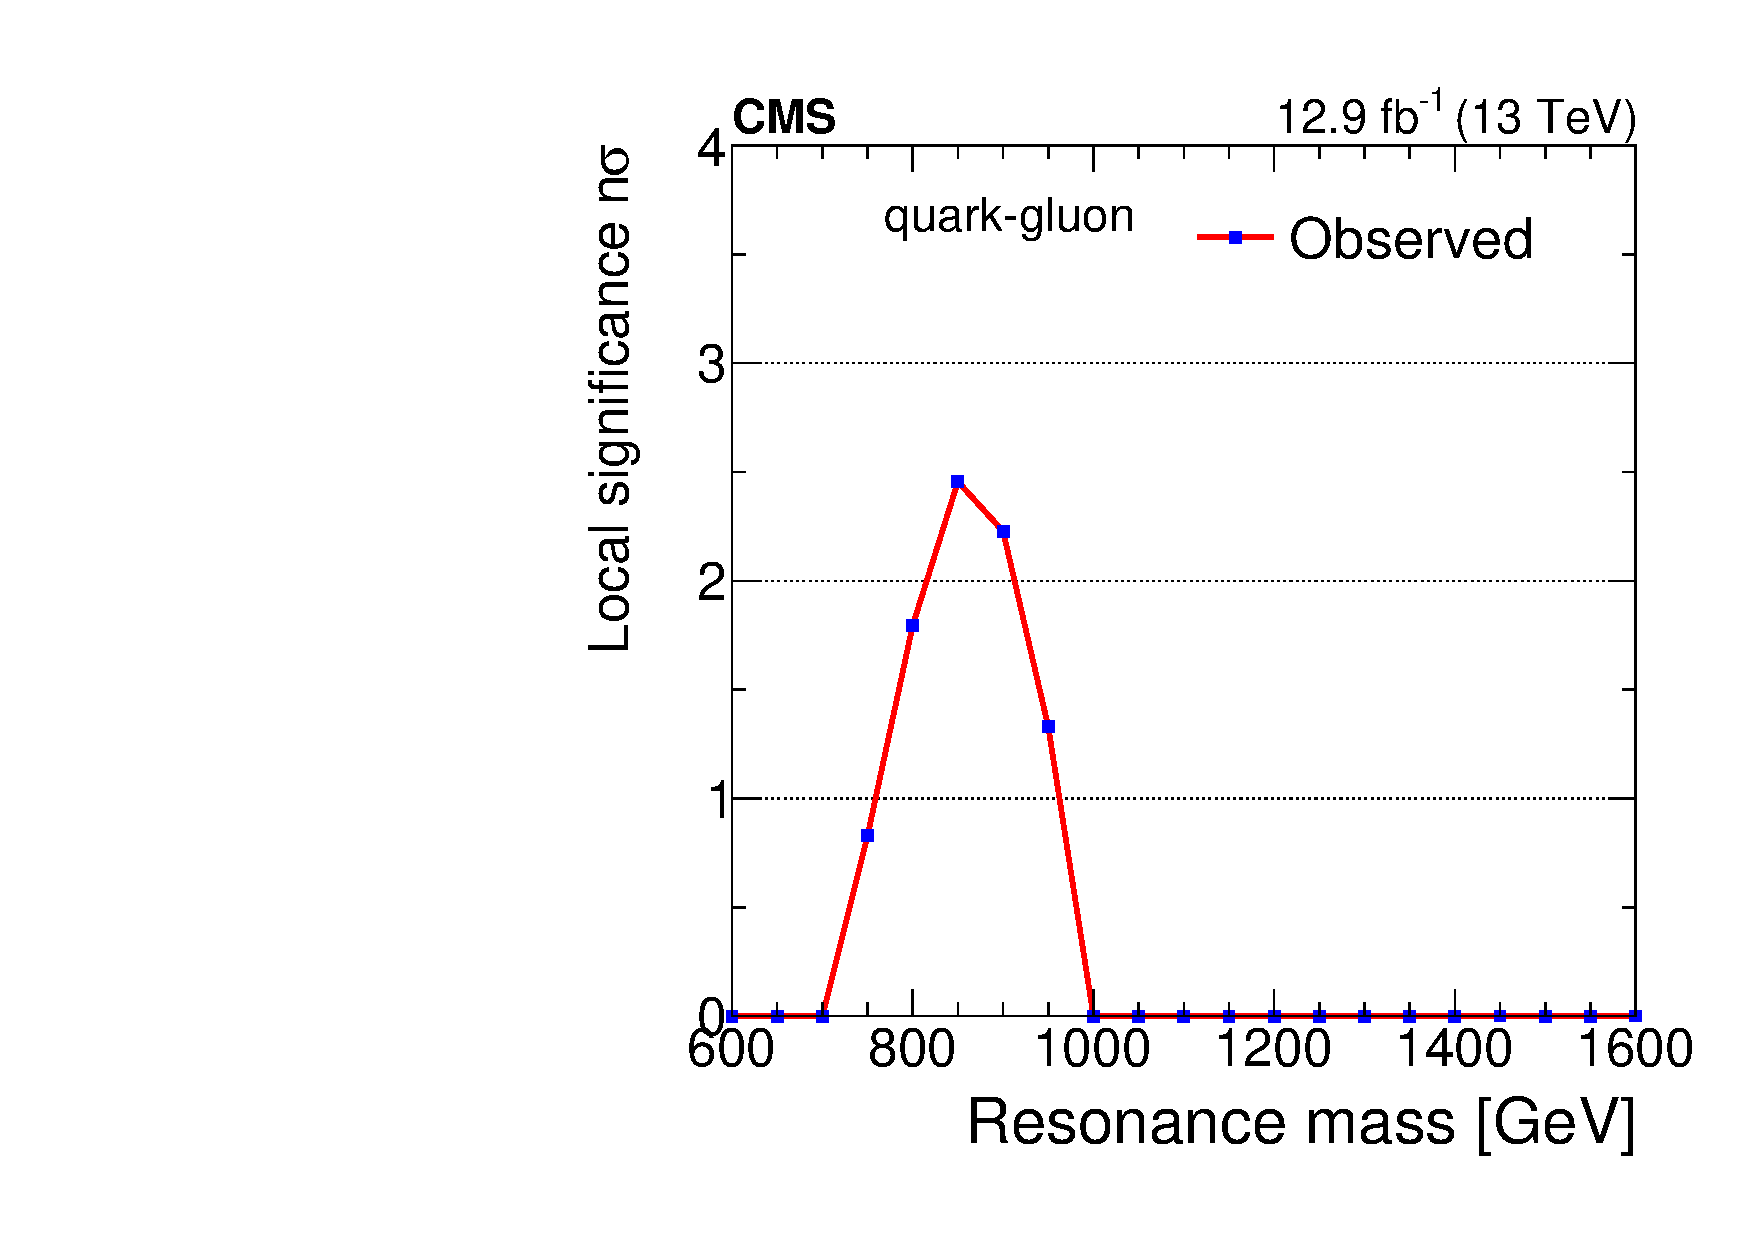
\includegraphics[width=0.48\textwidth]{figs/dijet/signif_qg_calodijet2016.pdf}
    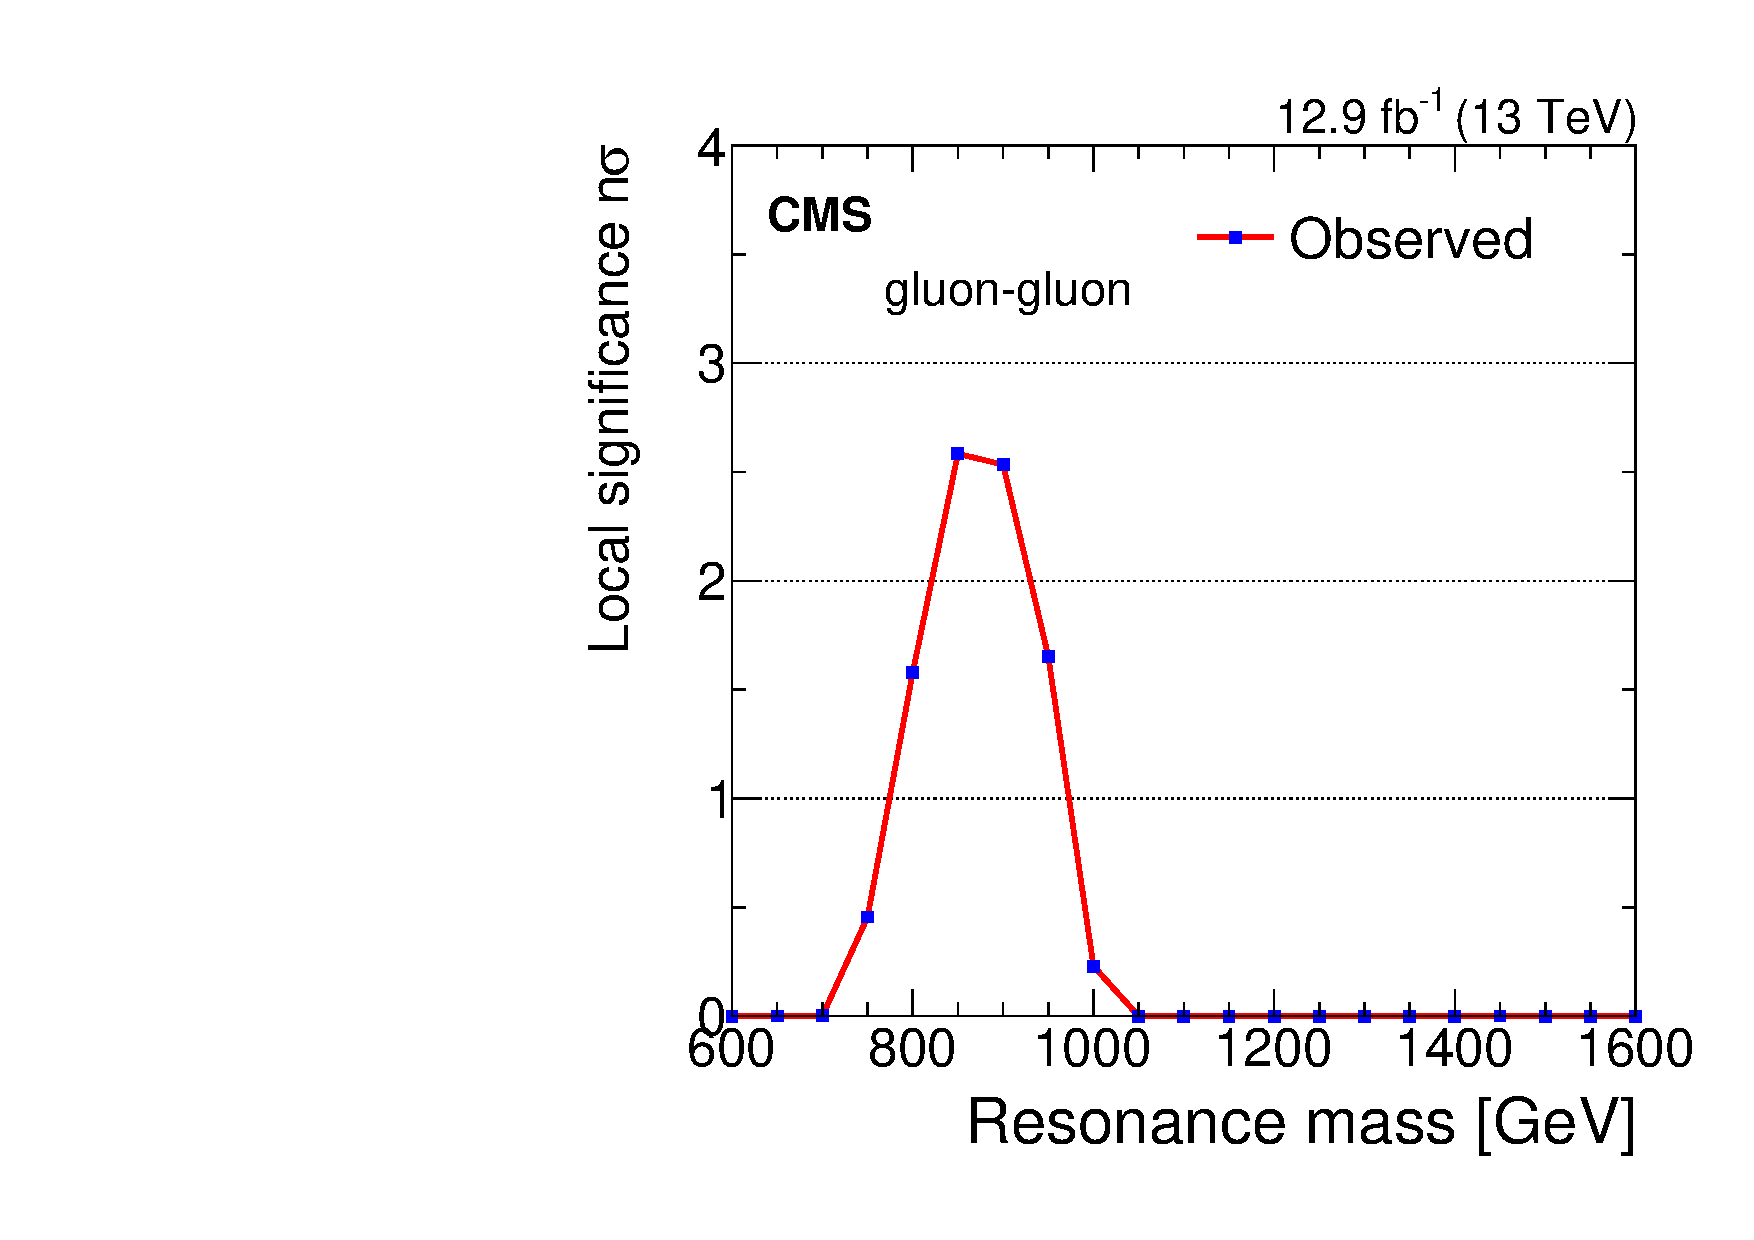
\includegraphics[width=0.48\textwidth]{figs/dijet/signif_gg_calodijet2016.pdf}
    \caption{Observed signal significance from the low-mass search for
      quark-quark (top left), quark-gluon (top right), and gluon-gluon
      (bottom) type dijet resonances~\cite{jmgd}.}
    \label{figSignifLow}
\end{figure*}

\begin{figure*}[hbtp]
  \centering
    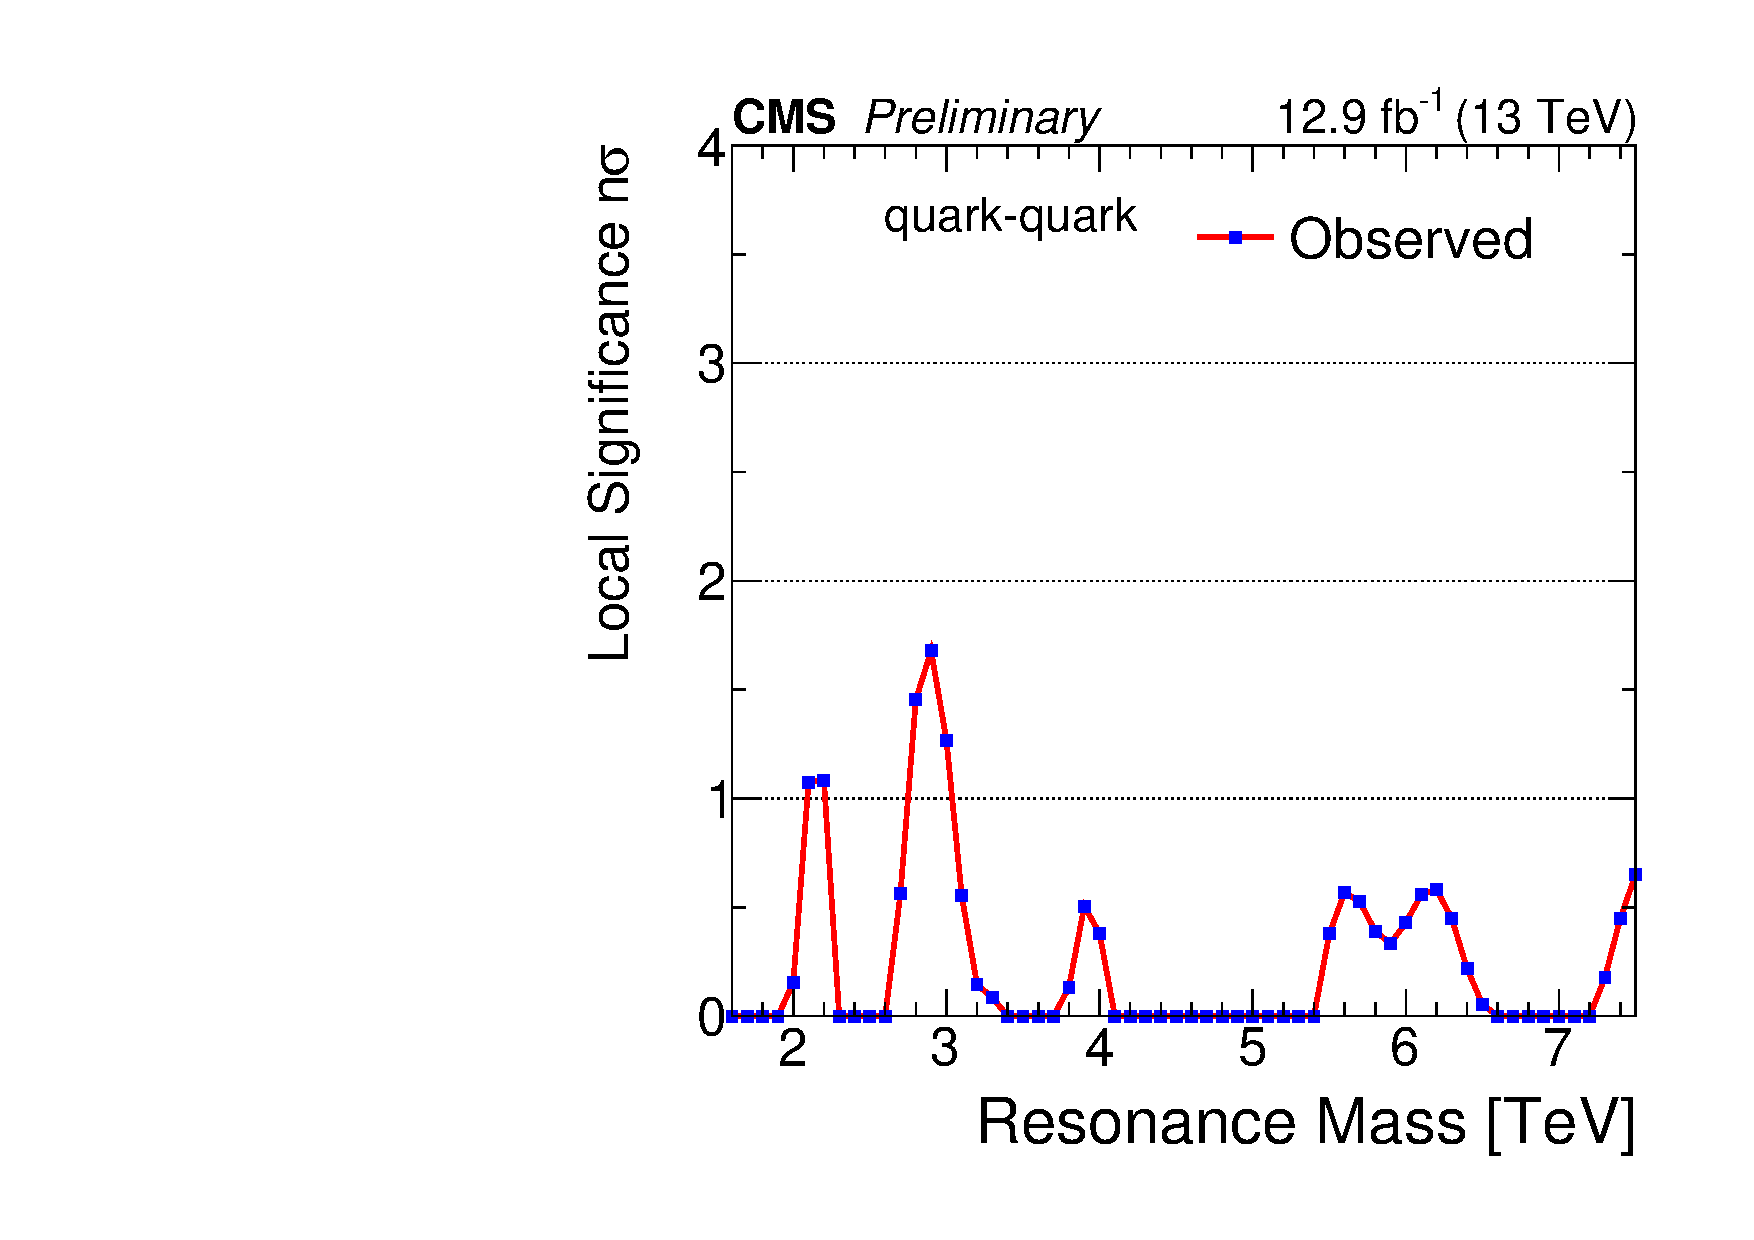
\includegraphics[width=0.48\textwidth]{figs/dijet/signif_qq_pfdijet2016.pdf}
    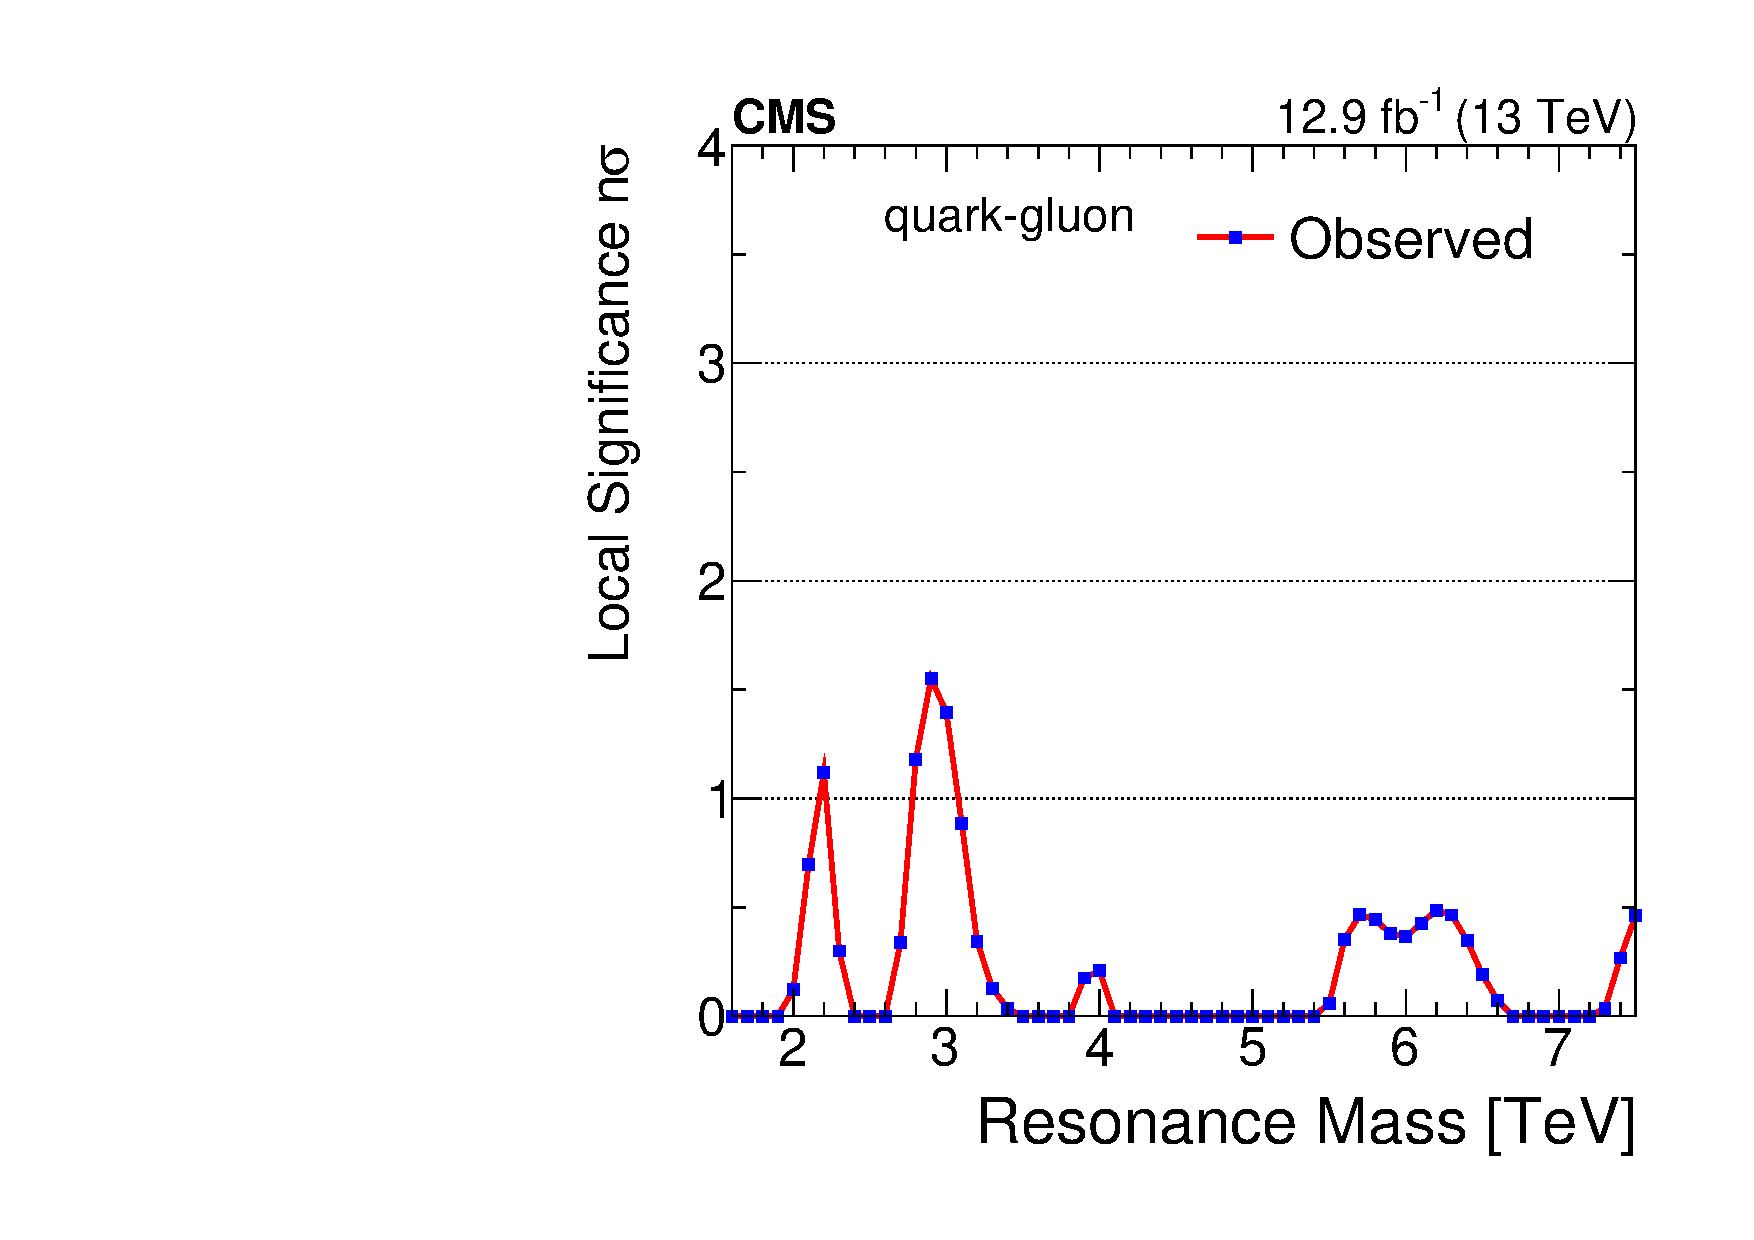
\includegraphics[width=0.48\textwidth]{figs/dijet/signif_qg_pfdijet2016.pdf}
    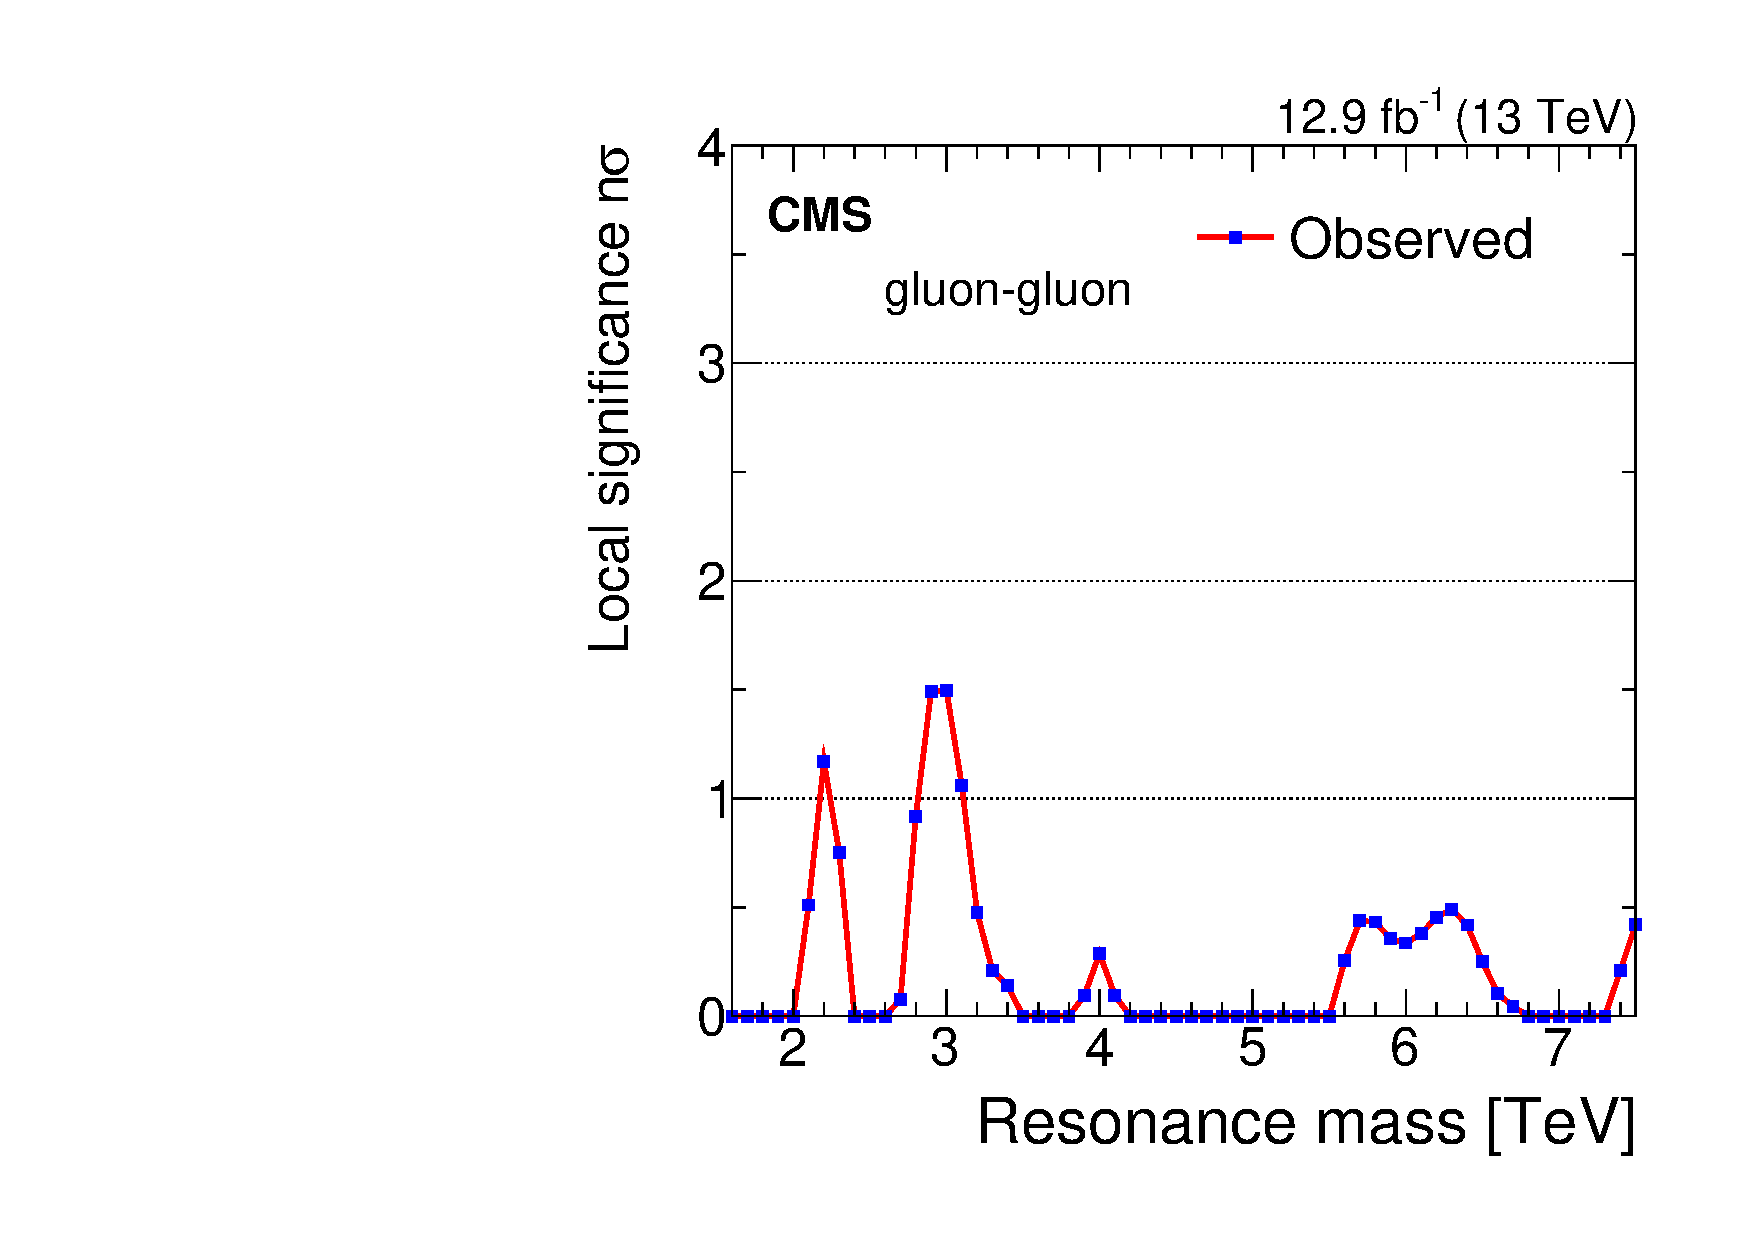
\includegraphics[width=0.48\textwidth]{figs/dijet/signif_gg_pfdijet2016.pdf}
    \caption{Observed signal significance from the high-mass search for
      quark-quark (top left), quark-gluon (top right), and gluon-gluon
      (bottom) type dijet resonances~\cite{jmgd}.}
    \label{figSignifHigh}
\end{figure*}

Figures~\ref{figLimitLow}-\ref{figLimitAll} and
Tables~\ref{tab:limits}-\ref{tab:pflimits} show the model-independent observed
upper limits at 95\% confidence level (\CLp) on
$\sigma\times B\times A$, i.e., the product of
the cross section ($\sigma$), the branching fraction ($B$), and the acceptance ($A$) for the
kinematic requirements $\detajj<1.3$ and $\abs{\eta}<2.5$,
for narrow resonances. 
In Fig.~\ref{figLimitLow}, for comparison purposes only, limits are also shown from Gaussian shapes with 
an RMS width equal to 10\% of the mass.
The acceptance of the minimum dijet mass requirement in each search has been taken into account
by correcting the limits, and therefore does not appear in the acceptance $A$.
Figures~\ref{figLimitLow}-\ref{figLimitAll} also show the expected limits on the cross section and their bands of uncertainty.
The generated mass spectra are fit with a signal-plus-background model to extract expected upper limits.
The difference in the limits for $\PQq\PQq$, $\PQq\Pg$, $\Pg\Pg$ and Gaussian resonances at the same resonance mass
originates from the difference in their lineshapes. We note that the limits from Gaussian resonances are smaller
than can be expected from any physical model, as they do not have any tails due to radiation, and consequently they are narrower 
and located closer to the resonance pole than any combination of two
partons can produce. 

%We present limits with Gaussian shapes of 10\% width in order to compare the sensitivity of this search to
%the tails of the signal shape, and the sensitivity
%of these results with those from ATLAS in Ref.~\cite{ATLAS-CONF-2016-030} which presents results 
%using the same Gaussian shape.  We find a similar sensitivity between
%the two experiments. We note, however, that these Gaussian shapes are
%unrealistic as they neglect the sizable tails due to QCD radiation, and are consequently more narrow and result in 
%significantly better limits than can be physically expected for any pair of partons.  
%The limit on $\sigma\times B\times A$ with the Gaussian shape of 10\% width at 750 GeV is 1.8 pb
%expected, and the previous ATLAS limit in Ref.~\cite{ATLAS-CONF-2016-030} was 2.4 pb for a luminosity of 3.4 \fbinv. We note that the ATLAS 
%analysis used $\detajj<1.2$ which gives 93\% of the acceptance of CMS for an isotropic signal.  After adjusting for differences 
%in luminosity and acceptance between the two analyses the CMS and ATLAS sensitivities to a Gaussian resonance of mass 750 GeV and width 10\% are 
%similar.  We also note that at this resonance mass for this signal shape our reported limit, which includes systemic uncertainties, is 60\% larger 
%than the limit obtained without including systematic uncertainties. 
%For a gluon-gluon resonance at a mass of 750 GeV, systematic uncertainties increase the limit by a factor of 3, a significantly larger effect than
%for a Gaussian resonance which neglects the effect of radiation. Our limits on hypothetical Gaussian resonances
%are only recommended for such comparisons, 
%as we have demonstrated that these Gaussian shapes neglect the sizable tails due to QCD radiation, and are consequently more narrow and result in 
%significantly better limits than can be physically expected for any pair of partons.  

Figures~\ref{figSignifLow}~and~\ref{figSignifHigh} also show the observed
signal significance as a function of resonance mass for both
searches. No sizeable significance is found, with the largest being
$2.6\sigma$ for an $850\GeV$ $\Pg\Pg$ resonance.

\section{Model-dependent interpretation}

All upper limits presented can be compared to the parton-level predictions of $\sigma\times B\times A$, without detector simulation,
to determine mass limits on new particles.
The model predictions shown in Fig.~\ref{figLimitLow}-\ref{figLimitAll} are calculated in the narrow-width
approximation~\cite{Harris:2011bh} using the CTEQ6L1~\cite{refCTEQ} PDF at leading order,
with a next-to-leading order correction factor included for the $\PWpr$, $\PZpr$, and axigluon/coloron models~\cite{Chivukula:2013xla}. 
The acceptance is evaluated at the parton level for the resonance decay to two partons. In the case of isotropic
decays it is $A\approx 0.6$ independent of resonance mass.
For a given model, new particles are excluded at 95\% \CL in mass regions where the theoretical prediction
lies at or above the observed upper limit for the appropriate final state of Fig.~\ref{figLimitLow}-\ref{figLimitAll}.
For the RS graviton model, for which 60\% (40\%) of the cross section comes from sub-proceses with 
only quarks (gluons) in the final state, we obtain mass limits by comparing the RS graviton
cross section curve to a weighted average of the limits in the quark-quark and gluon-gluon final states.
Mass limits on all benchmark models are summarized in Table~\ref{tab:MassLimit} and are more stringent than the mass limits previously published by 
CMS~\cite{Khachatryan:2015dcf} and ATLAS~\cite{ATLAS:2015nsi} in the dijet channel. 

\begin{table}[ht]
  \caption{ Observed and expected mass limits at 95\% CL from this analysis with \RunLumi at $\sqrt{s}=13$\TeV 
  compared to previously published limits on narrow resonances from CMS with 2.4\fbinv at $\sqrt{s}=13$\TeV~\cite{Khachatryan:2015dcf} 
  and  with 20\fbinv at $\sqrt{s}=8$\TeV~\cite{Khachatryan:2015sja}. The listed models are excluded between \minMassLow 
  and the indicated mass limit by this analysis. For the $\PZpr$ model, in addition to the observed mass limit
  listed below, this analysis also excludes the mass interval between 2.3 and 2.6 \TeV.}
  \centering
\resizebox{\textwidth}{!}{
  \begin{tabular}{lcccc}\hline\hline
          &                                 & \multicolumn{3}{c}{Observed (expected) mass limit [\TeVns{}]} \\
    Model & Final                           & \RunLumi      & 2.4\fbinv      & 20\fbinv \\
          & State                           & 13\TeV        & 13\TeV         & 8\TeV \\
    \hline
String   & $\PQq\Pg$                        & 7.4\ (7.4)    & 7.0\ (6.9)     & 5.0\ (4.9)\\
Scalar diquark  & $\PQq\PQq$                & 6.9\ (6.8)    & 6.0\ (6.1)     & 4.7\ (4.4)\\
Axigluon/coloron  & $\PQq\PAQq$             & 5.5\ (5.6)    & 5.1\ (5.1)     & 3.7\ (3.9)\\
Excited quark  &  $\PQq\Pg$                 & 5.4\ (5.4)    & 5.0\ (4.8)     & 3.5\ (3.7)\\
Color-octet scalar ($k_s^2=1/2$) & $\Pg\Pg$ & 3.0\ (3.3)    & ---            & --- \\
$\PWpr$ & $\PQq\PAQq$                       & 2.7\ (3.1)    & 2.6\ (2.3)     & 2.2\ (2.2)\\
$\PZpr$ & $\PQq\PAQq$                       & 2.1\ (2.3)    & ---            & 1.7\ (1.8)\\
DM mediator ($m_\mathrm{DM} = 1\GeV$) & $\PQq\PAQq$                       & 2.0\ (2.0)    & ---            & ---  \\
RS Graviton  & $\PQq\PAQq$, $\Pg\Pg$        & 1.9\ (1.8)    & ---            & 1.6\ (1.3)\\\hline\hline
 \end{tabular}}
\label{tab:MassLimit}
\end{table}

Following the theoretical framework of Ref.~\cite{Dobrescu:2013coa},
the upper limits on the cross section of narrow $\PQq\PQq$ resonances are
translated into 95\% CL upper limits on the coupling
$g_\mathrm{B}$ of a hypothetical leptophobic resonance $\PZpr_\mathrm{B} \to\Pq \PAQq$
as a function of its mass.  The $\PZpr_\mathrm{B}$ production cross section
scales with the square of the coupling $g_\mathrm{B}$.  Fig.~\ref{fig:gBvsMZ}
shows the upper limits obtained with the low-mass search in
the mass region from 600 to 1600\GeV and with the high-mass search in
the mass region from 1.6 \TeV to 3.7\TeV. The limits are competitive with the
coverage of previous CMS searches at $\sqrt{s}=8
\TeV$~\cite{Khachatryan:2016ecr} in the low-mass range and improve
upon previous limits in the high-mass range. Previous exclusions obtained with
similar searches at various collider energies~\cite{Khachatryan:2016ecr,ATLAS:2015nsi,Dobrescu:2013coa,Aad:2014aqa} are also shown. 
%As a result of the large data set collected by the data scouting stream,
%the bound on $g_\mathrm{B}$ is improved by up to a factor of 3 for resonance
%masses between 500 and 800\GeV, compared to previous searches. This
%corresponds to an order-of-magnitude improvement in the cross section
%limit.

% width is a sub-case of the one discussed below. multiplied by 5 for
% each quark flavor u, d, c, s, b
%\begin{equation}
%\Gamma(\Zpr_B\to jj) = 5 \frac{g_\mathrm{B}^2m_{\Zpr_B}}{36(4\pi)}\left(1+\frac{\alpha_s}{\pi}\right)
%\end{equation}

\begin{figure}
\centering
%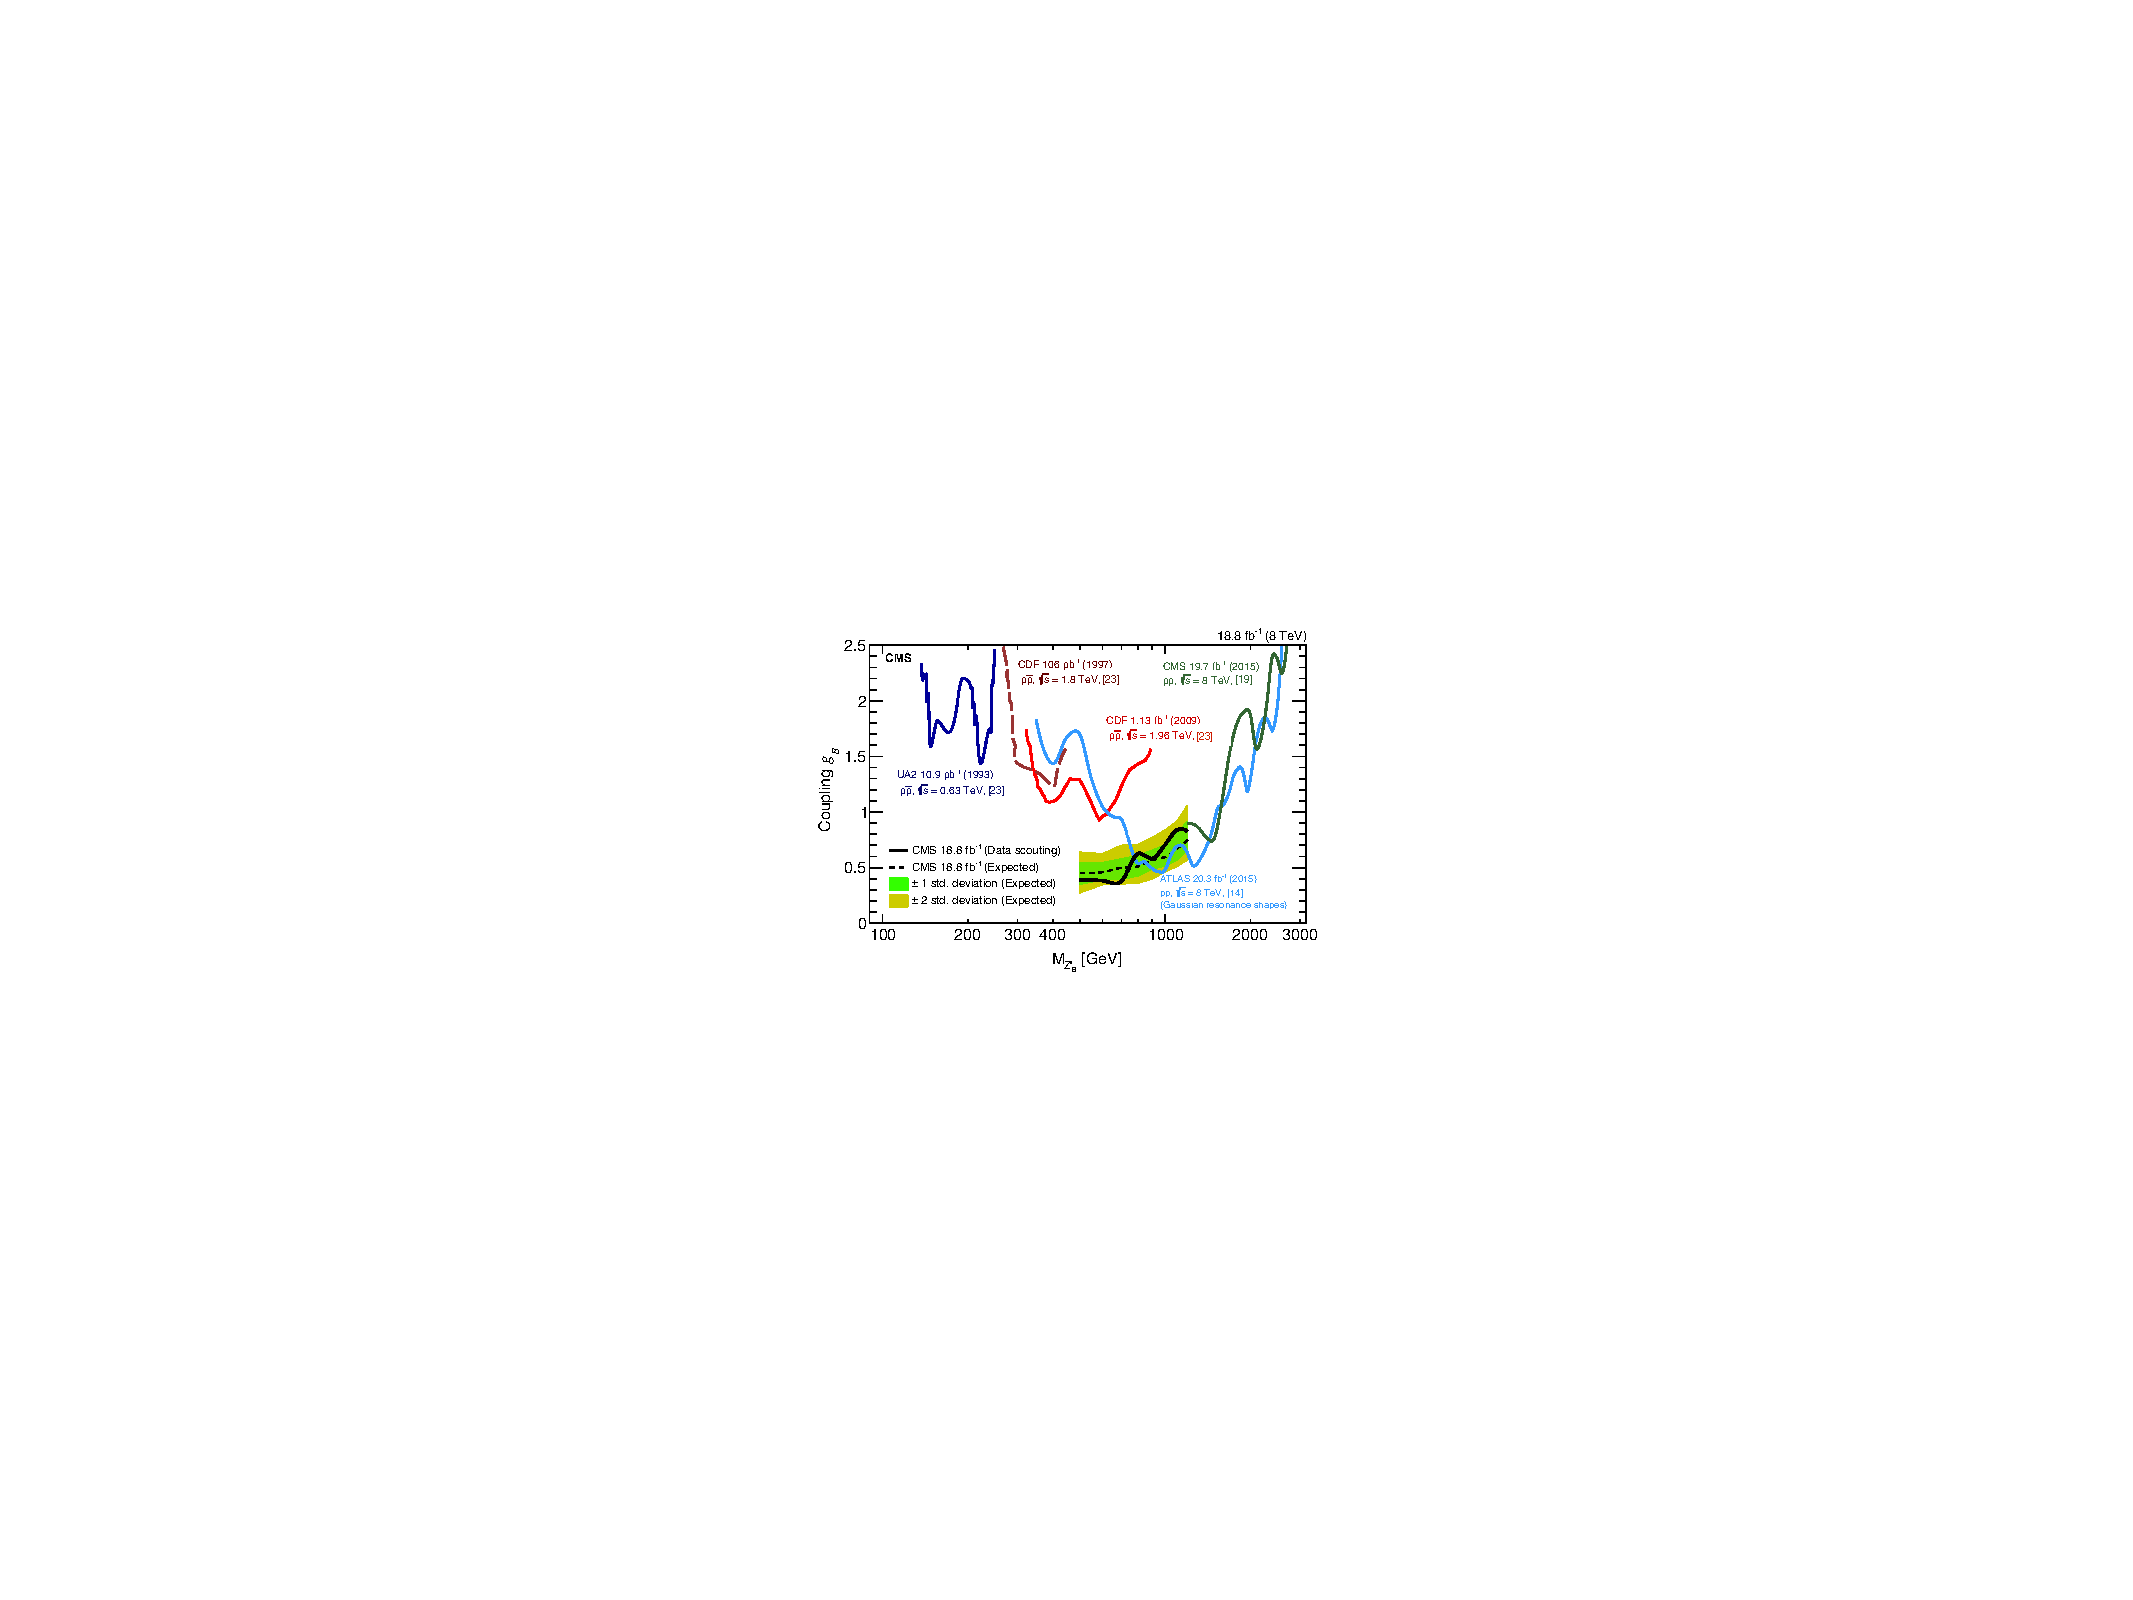
\includegraphics[width=0.9\textwidth]{figs/dijet/gB_Limits_ALL_with_uncertainty.pdf}
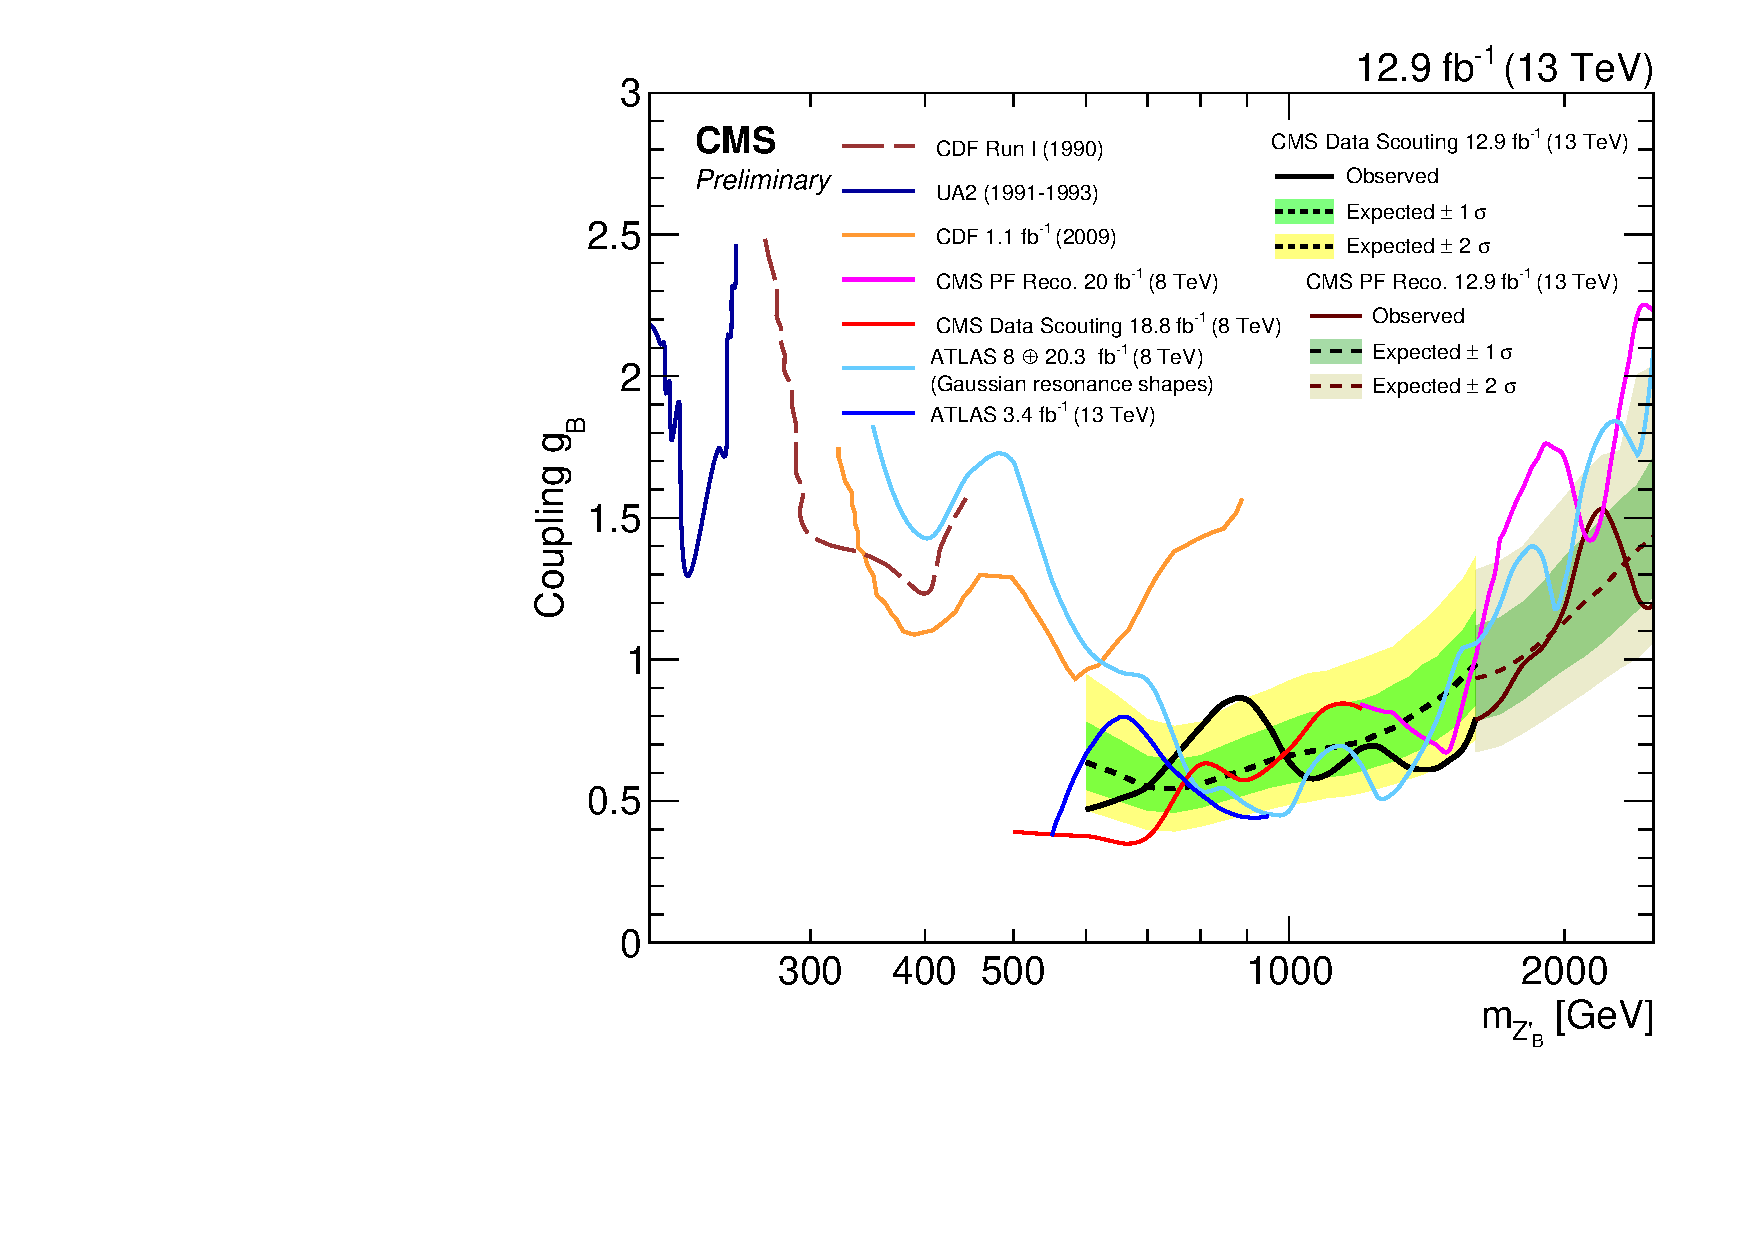
\includegraphics[width=0.9\textwidth]{figs/dijet/gB_Limits_12_9_ifb.pdf}
\caption{Observed 95\% \CLp~upper limits on the coupling $g_\mathrm{B}$ of a hypothetical leptophobic
resonance $\PZpr_\mathrm{B} \to\PQq \PAQq$~\cite{Dobrescu:2013coa} as a
function of its mass~\cite{jmgd}. The results from this study are compared to
results obtained with similar searches at different collider
energies~\cite{Khachatryan:2016ecr,ATLAS:2015nsi,Dobrescu:2013coa,Aad:2014aqa}.\label{fig:gBvsMZ}}
\end{figure}

The results of the dijet search also have an impact on the allowed
parameter space in models of dark matter (DM) production at the
LHC if the mediator is also accessible.
We may use a similar simplified model to quantify this impact,
consisting of a leptophobic vector (V) or axial-vector (AV) mediator
$\PZpr_\mathrm{B}$ with couplings to quarks and the DM particle $\chi$~\cite{Boveia:2016mrp,Dobrescu:2013coa,Abercrombie:2015wmb}:
\begin{align}
\mathcal L_\mathrm{V} &=
                        -g_{\mathrm{DM}}Z^{\prime}_{B\mu}\overline\chi\gamma^{\mu}\chi
                        - g^{\prime}_{\Pq}\sum_{\Pq}Z^{\prime}_{B\mu}\bar q\gamma^{\mu} q~,\\
\mathcal L_\mathrm{AV} &= -g_{\mathrm{DM}}Z^{\prime}_{B\mu}\overline\chi\gamma^{\mu}\gamma_5\chi-g^{\prime}_{\Pq}\sum_{\Pq}Z^{\prime}_{B\mu}\bar q\gamma^{\mu} \gamma_5q~,
\end{align}
where $g_{\mathrm{DM}}$ is the coupling of the mediator to the DM
particles and $g_{\Pq}^{\prime}=g_\mathrm{B}^{\prime}/6$ is the universal
coupling of all quark flavors to the mediator. Fig.~\ref{fig:OP} shows
the most important diagrams for monojet and dijet searches.

\begin{figure}[h!]
\centering
  \unitlength=0.005\textwidth
  \vspace{\baselineskip}
  \begin{feynmandiagram}[modelVmonojetParameters]
    \fmfleft{i1,i2}
    \fmfright{o1,o2}
    \fmftop{isr}
    \fmfbottom{pisr}
    \fmf{wiggly,tension=0.6,label={ $\PZpr_\mathrm{B}(\mMed)$}}{v1,v2}
    \fmf{fermion}{o2,v2,o1}
    \fmf{fermion}{i2,visr,v1}
    \fmf{plain}{v1,pvisr,i1}
    \fmf{fermion,tension=0}{v1,i1}
    \fmfdot{v1,v2}
    %\fmfdot{v1,v2,visr}
    \fmflabel{ ${\gq^{\prime}}$}{v1}
    \fmflabel{ ${\gDM}$}{v2}
    \fmflabel{ ${\Paq}$}{i1}
    \fmflabel{ ${\Pq}$}{i2}
    \fmflabel{ ${\overline{\chiDM}(\mDM)}$}{o1}
    \fmflabel{ ${\chiDM(\mDM)}$}{o2}
    %\fmflabel{ $\alpha_{\mathrm{s}}$}{visr}
    \fmfv{decor.shape=circle,decor.filled=full,decor.size=2thick,label=$g_{\mathrm{s}}$,label.angle=180}{visr}
    \fmf{gluon,tension=0}{visr,isr}
    \fmf{phantom,tension=0}{pvisr,pisr}
    \fmflabel{ ${\Pg}$}{isr}
  \end{feynmandiagram}\hfill
  \begin{feynmandiagram}[modelVdijetParameters]
    \fmfleft{i1,i2}
    \fmfright{o1,o2}
    \fmftop{isr}
    \fmfbottom{pisr}
    \fmf{wiggly,tension=0.6,label.side=right,label={ $\PZpr_\mathrm{B}(\mMed)$}}{v1,v2}
    \fmf{fermion}{o2,v2,o1}
    \fmf{fermion}{i2,v1}
    \fmf{plain}{v1,i1}
    \fmf{fermion,tension=0}{v1,i1}
    \fmfdot{v1,v2}
    \fmflabel{ ${\gq^{\prime}}$}{v1}
    \fmflabel{ ${\gq^{\prime}}$}{v2}
    \fmflabel{ ${\Paq}$}{i1}
    \fmflabel{ ${\Pq}$}{i2}
    \fmflabel{ $\Paq$}{o1}
    \fmflabel{ $\Pq$}{o2}
  \end{feynmandiagram}
  \vspace{\baselineskip}
\caption{Representative Feynman diagrams showing the pair production of
  dark matter particles in association with a radiated gluon from the initial
  state used in $\MET+\mathrm{X}$ (mono-X) searches (left) and the
  pair production of quarks used in dijet searches (right) via a
  vector or axial-vector $\PZpr_\mathrm{B}$ mediator~\cite{jmgd}. The cross section and kinematics depend on the mediator and dark
matter masses, and the mediator couplings to dark matter and quarks, 
respectively: ($\mMed ,\, \mDM ,\, \gDM ,\,
\gq^{\prime}$)~\cite{Abercrombie:2015wmb}. \label{fig:OP}}
\end{figure}

%For V and AV models we follow section 2.1 and S
%and PS models we use the definition provided in section 2.2 of
%Ref.~\cite{Boveia:2016mrp}. 
%As the reinterpretation of pure mediator searches like the CMS dijet
%analysis requires to take into account different final states
%(e.g. quarks and DM), we repeat here the definition of the V and AV
%that are used to compare mediator searches like dijets with \MET
%based DM searches like monojets. 
The results of the search for a narrow $\Pq\Paq$ resonance may then be reinterpreted as a search for
the mediator when it decays to quarks. In this model, the minimal decay width of the mediator is given by the sum of the partial widths for
all decays into DM particles and quarks that are kinematically
accessible, which we take to be $\Pq=\PQu,\PQd,\PQc,\PQs,\PQb$: 
\begin{equation}
\Gamma^{\mathrm{tot}} =
\Gamma^{\chi\overline\chi} + 3 \sum_{\Pq} \Gamma^{\Pq\Paq}~.
\end{equation}
The partial widths are given by:
\begin{align}
\Gamma^{\chi\overline\chi}_{\mathrm{V}} &=
\frac{g^2_{\mathrm{DM}}m_{\mathrm{med}}}{12\pi} \left ( 1 - 4
  \frac{m^2_{\mathrm{DM}}}{m^2_{\mathrm{med}}}  \right )^{1/2} \left ( 1 + 2
  \frac{m^2_{\mathrm{DM}}}{m^2_{\mathrm{med}}}  \right ) ~,\\
\Gamma^{\chi\overline\chi}_{\mathrm{AV}} &=
\frac{g^2_{\mathrm{DM}}m_{\mathrm{med}}}{12\pi} \left ( 1 - 4
  \frac{m^2_{\mathrm{DM}}}{m^2_{\mathrm{med}}}  \right )^{3/2} ~,\\
\Gamma^{\Pq\Paq}_{\mathrm{V}} &=
\frac{(g^{\prime}_{\Pq})^2m_{\mathrm{med}}}{4\pi} \left ( 1 - 4
  \frac{m^2_{\Pq}}{m^2_{\mathrm{med}}}  \right )^{1/2}\left ( 1 + 2
  \frac{m^2_{\Pq}}{m^2_{\mathrm{med}}}  \right ) ~,\\
\Gamma^{\Pq\Paq}_{\mathrm{AV}} &=
\frac{(g^{\prime}_{\Pq})^2m_{\mathrm{med}}}{4\pi} \left ( 1 - 4
  \frac{m^2_{\Pq}}{m^2_{\mathrm{med}}}  \right )^{3/2} ~,
\end{align}
where $m_{\mathrm{med}}$ is the mediator mass, $m_{\mathrm{DM}}$ is
the mass of the DM particle, which is assumed to be a Dirac fermion,
and $m_{\Pq}$ is the quark mass. The two different types
of contribution to the total width vanish for $m_{\mathrm{med}} < 2
m_{\mathrm{DM}}$ and $m_{\mathrm{med}} < 2 m_{\Pq}$, respectively.

To derive the limit on $g_\mathrm{B}^{\prime}$ in this model in the case of
a nonzero mediator decay width to DM particles $\Gamma^{\chi\overline\chi}$, it
is simplest to begin with the limit on $g_\mathrm{B}$ in the case of zero decay
width to DM particles (see Fig.~\ref{fig:gBvsMZ}) and correct for the DM width,
\begin{align}
&&\sigma[\PZpr_\mathrm{B}\to\Pq\Paq|g_\mathrm{B}^{\prime},g_{\mathrm{DM}}] &=\sigma(\PZpr_\mathrm{B}\to\Pq\Paq| g_\mathrm{B}, g_{\mathrm{DM}}=0) \\
&\Rightarrow& \frac{(g_\mathrm{B}^{\prime})^4}{\Gamma^{\Pq\Paq}(g_\mathrm{B}^{\prime}) +
  \Gamma^{\chi\overline\chi}}& =\frac{g_\mathrm{B}^4}{\Gamma^{\Pq\Paq}(g_\mathrm{B})} \\
&\Rightarrow& (g^{\prime}_B)^2&=\frac{g_\mathrm{B}^2}{2}\left(1 + \sqrt{1+ 4\frac{\Gamma^{\chi\overline\chi}}{\Gamma^{\Pq\Paq}(g_\mathrm{B})}}\right )~.
\end{align}

Fig.~\ref{fig:DMsummary} shows 95\% CL exclusion regions in
($m_{\mathrm{med}}$,$m_{\mathrm{DM}}$) plane for dijet
  searches~\cite{CMS-PAS-EXO-16-032,Khachatryan:2016ecr} and
  different $\MET$ based DM searches~\cite{CMS-PAS-EXO-16-030,CMS-PAS-EXO-16-037,CMS-PAS-EXO-16-039,CMS-PAS-EXO-16-010} from CMS in the leptophobic
 vector and  axial-vector models defined above. Following the
  recommendation of the LHC DM working
  group~\cite{Boveia:2016mrp,Abdallah:2015ter,Abercrombie:2015wmb}, the exclusions are
  computed for a universal quark coupling $g_{\Pq}^{\prime} = 0.25$ and for a DM
  coupling of $g_{\mathrm{DM}} = 1.0$.
%The CMS dijet searches are reinterpreted using the model prediction after applying the kinematic cuts of the search on
%generator-level events and comparing it to the observed and expected
%exclusions on $\PQq\PAQq$ resonances. 
The combination of the low- and high-mass searches as well as the
search of Ref.~\cite{Khachatryan:2016ecr} excludes all values
of DM particle mass between 0.5 \TeV and 2.0 \TeV in mediator
mass. The expected mediator mass exclusion limit increases with
$m_{\mathrm{DM}}$ and goes as high as 2.7 \TeV for heavy DM particles
as the branching ratio to $\Pq\Paq$ dominates. The exclusion
limits are similar for the V and AV models, as expected. 

The search results presented in Fig.~\ref{fig:DMsummary} can also be compared with results
from dark matter direct detection (DD) and indirect detection (ID) experiments~\cite{Boveia:2016mrp}. As input for this
comparison, we use the results for the ($m_{\mathrm{med}}$,$m_{\mathrm{DM}}$) plane for fixed
couplings $g^{\prime}_{\Pq}$ and $g_{\mathrm{DM}}$. To compare with DD
and ID experiments, these limits are translated into the planes of DM mass versus the spin-independent
(SI) or spin-dependent (SD) DM-nucleon cross section,
$\sigma^{\mathrm{SI}}_{\mathrm{DM\textrm{-}\PN}}$ or $\sigma^{\mathrm{SD}}_{\mathrm{DM\textrm{-}\Pp}}$, respectively. The SI
DM-nucleon cross section takes the form~\cite{Boveia:2016mrp}:
\begin{align}
\sigma^{\mathrm{SI}}_{\mathrm{DM\textrm{-}\PN}}& = \frac{f^2(g^\prime_\Pq) g_\mathrm{DM}^2
  \mu_{\PN\chi}}{\pi m_{\mathrm{med}}^4}\\
&\simeq 6.9\times10^{-41}\unit{cm}^2 \cdot \left (\frac{g^\prime_\Pq
  g_\mathrm{DM}}{0.25} \right)^2 \left (\frac{1 \TeV}{m_\mathrm{med}}
  \right)^4 \left (\frac{\mu_{\PN\chi}}{1\GeV} \right)^2 ~,
\end{align}
where $\mu_{\PN\chi} =
m_\PN m_\mathrm{DM}/(m_\PN+m_\mathrm{DM})$ is the
DM-nucleon reduced mass with $m_\PN \simeq 0.939\GeV$, and for a
vector mediator, $f(g^\prime_\Pq) = 3 g^\prime_\Pq$. Similarly, the SD
DM-nucleon cross section can be written as~\cite{Boveia:2016mrp}:
\begin{align}
\sigma^{\mathrm{SD}}_{\mathrm{DM\textrm{-}\Pp}} &= \frac{3f^2(g^\prime_\Pq) g_\mathrm{DM}^2
  \mu_{\PN\chi}}{\pi m_{\mathrm{med}}^4}\\
&\simeq 2.4\times10^{-42}\unit{cm}^2 \cdot \left (\frac{g^\prime_\Pq
  g_\mathrm{DM}}{0.25} \right)^2 \left (\frac{1 \TeV}{m_\mathrm{med}}
  \right)^4 \left (\frac{\mu_{\PN\chi}}{1\GeV} \right)^2 ~,
\end{align}
where, in general, the factor $f(g^\prime_\Pq)$ could be different for protons
and neutrons and depends separately on the individual quark-mediator couplings
$g^\prime_\PQu$, $g^\prime_\PQd$, and $g^\prime_\PQs$:
\begin{equation}
f^{\Pp,\Pn}(g^\prime_\PQu,g^\prime_\PQd,g^\prime_\PQs) = \Delta^{(\Pp,\Pn)}_\PQu g^\prime_\PQu + \Delta^{(\Pp,\Pn)}_\PQd g^\prime_\PQd +  \Delta^{(\Pp,\Pn)}_\PQs g^\prime_\PQs~,
\end{equation} 
with $\Delta^{(\Pp)}_\PQu=\Delta^{(\Pn)}_\PQd=0.84$,
$\Delta^{(\Pp)}_\PQd=\Delta^{(\Pn)}_\PQu=-0.43$, and
$\Delta^{(\Pp)}_\PQs=\Delta^{(\Pn)}_\PQs=-0.09$~\cite{Agashe:2014kda}. Under the assumption that the
coupling $g^\prime_\Pq$ is universal, these factors are equal, $f^{\Pp} = f^{\Pn} =0.32 g^\prime_\Pq$. As DD experiments quote 90\% CL limits, the CMS limits are also
recalculated to match this confidence level. Fig.~\ref{fig:DMsummary2}
shows the AV and V limits translated into the SD
and SI planes, respectively, and compared to DD and ID
experiments~\cite{Akerib:2016vxi,Tan:2016zwf,Agnese:2015nto,Angloher:2015ewa,Amole:2016pye,Amole:2015pla,Aartsen:2016exj,Choi:2015ara}. 

%It should be noted that the absolute exclusion regions of the different searches as well as their relative
%importance strongly depends on the chosen coupling and model
%scenario. Therefore, the exclusion regions, relic density contours,
%and unitarity curve shown in this plot are not applicable to other
%choices of coupling values or model.

\begin{figure}
\centering 
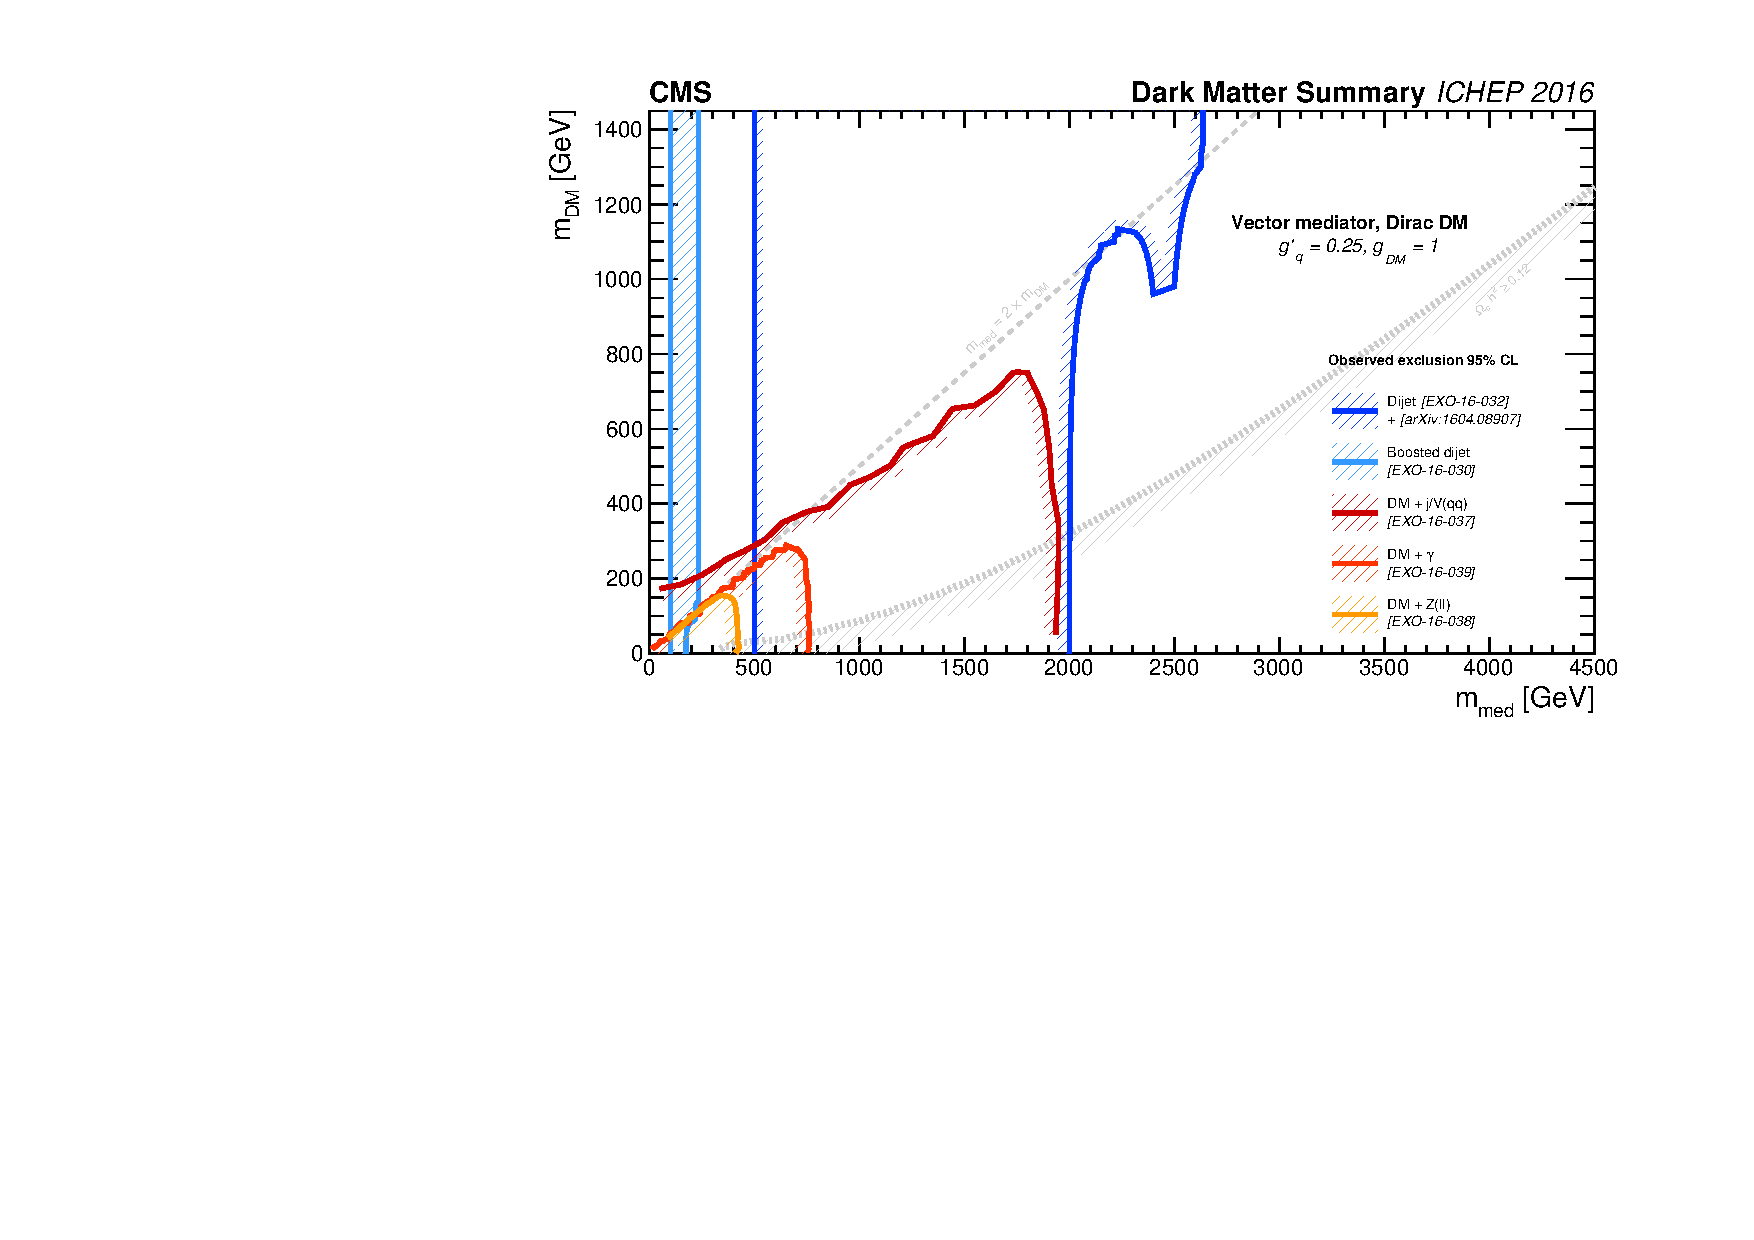
\includegraphics[width=0.95\textwidth]{figs/dijet/Vector_EXO_Summary_ICHEP.pdf}\\
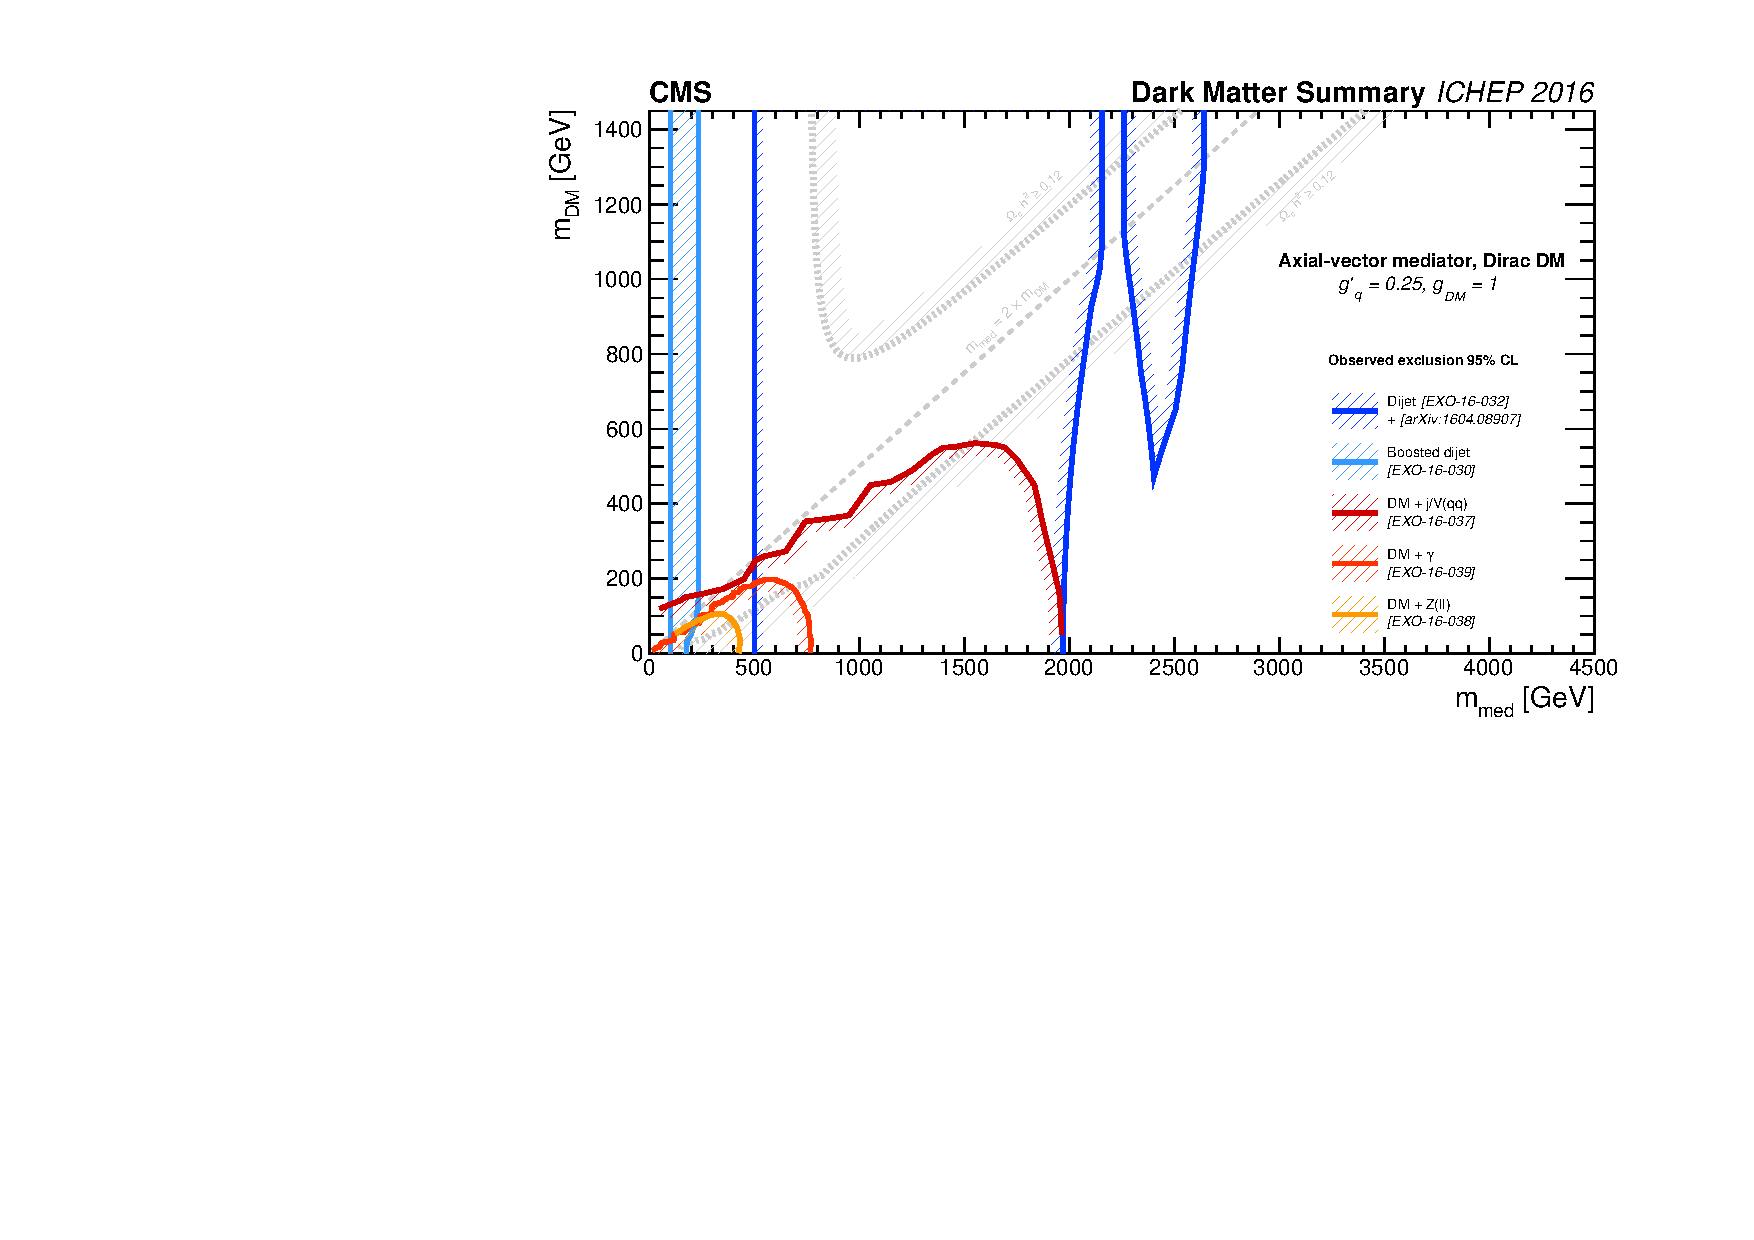
\includegraphics[width=0.95\textwidth]{figs/dijet/Axial_EXO_Summary_ICHEP.pdf}
\caption{95\% CL exclusion regions in
  ($m_{\mathrm{med}}$,$m_{\mathrm{DM}}$) plane for dijet
  searches~\cite{CMS-PAS-EXO-16-032,Khachatryan:2016ecr} and
  different $\MET$ based DM searches~\cite{CMS-PAS-EXO-16-030,CMS-PAS-EXO-16-037,CMS-PAS-EXO-16-039,CMS-PAS-EXO-16-010} from CMS in the leptophobic
  vector (top) and axial-vector (bottom) models~\cite{jmgd}. Following the
  recommendation of the LHC DM working
  group~\cite{Boveia:2016mrp,Abdallah:2015ter}, the exclusions are
  computed for a universal quark coupling $g^{\prime}_{\Pq} = 0.25$ and for a DM
  coupling of $g_{\mathrm{DM}} = 1.0$. It should be noted that the relic density
  contours, unitarity curves, and the exclusion regions of the
  different searches strongly depend on the chosen coupling and model
  scenario.\label{fig:DMsummary}}
\end{figure}


\begin{figure}
\centering 
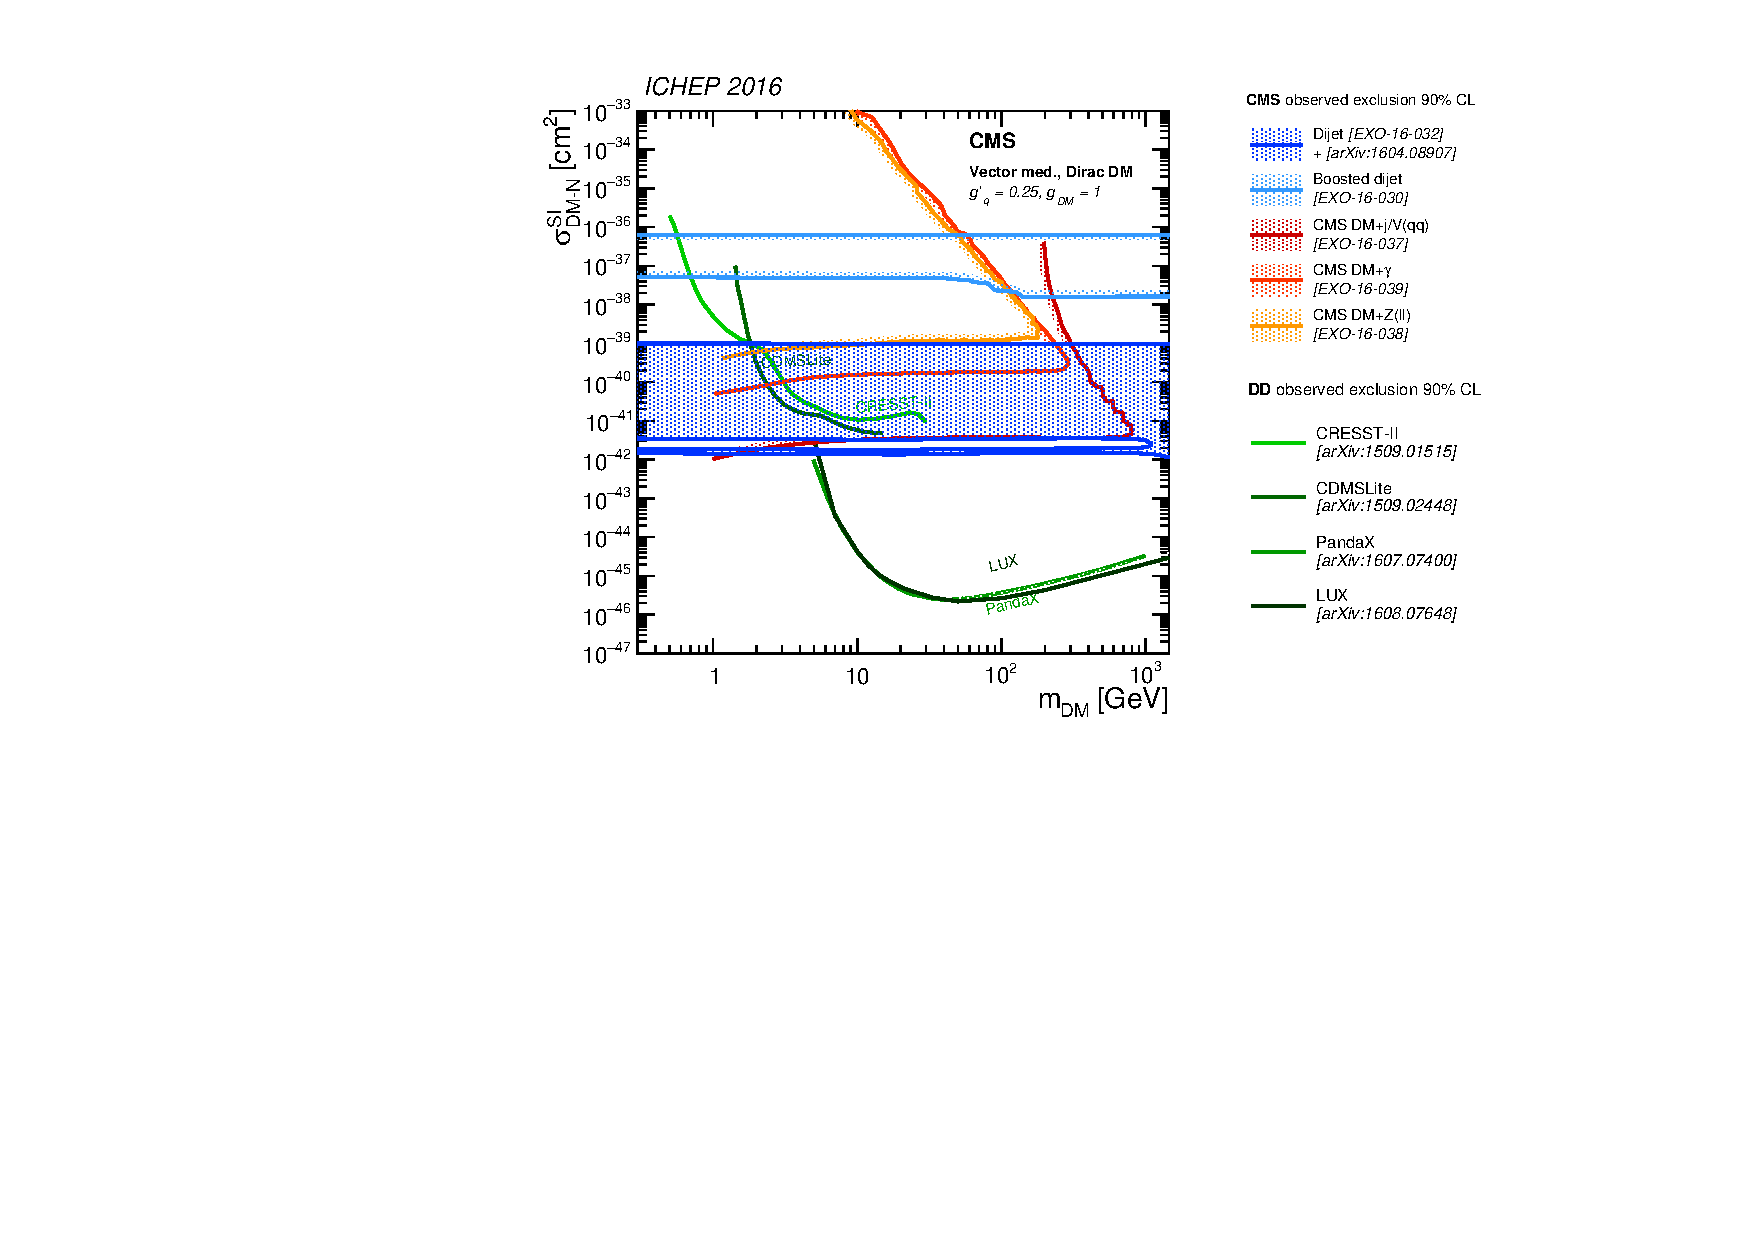
\includegraphics[width=0.95\textwidth]{figs/dijet/SI_CMSDD_Summary_ICHEP.pdf}\\
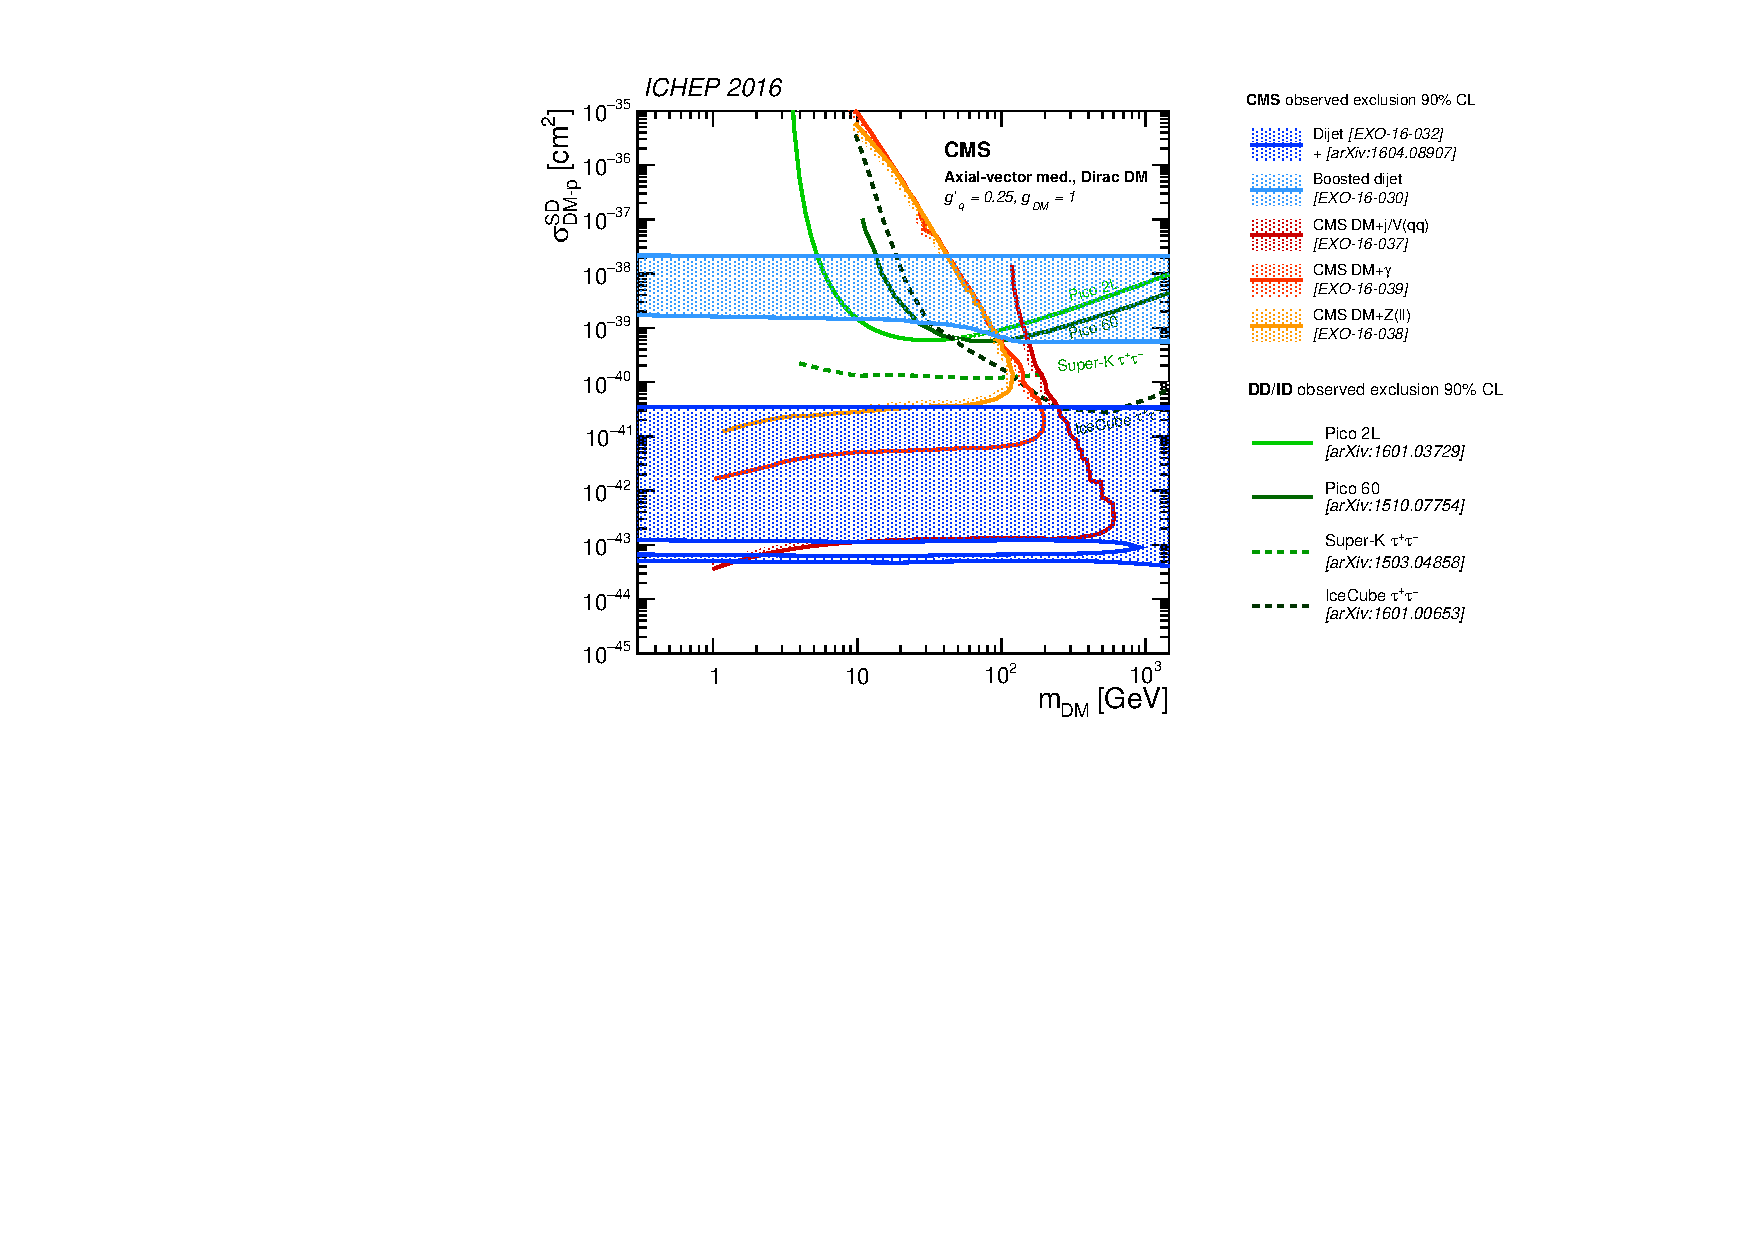
\includegraphics[width=0.95\textwidth]{figs/dijet/SD_CMSDD_Summary_ICHEP.pdf}
\caption{
A comparison of CMS results to direct and indirect dark matter
detection results in the ($m_{\mathrm{DM}}$,$\sigma^{\mathrm{SI}}_{\mathrm{DM\textrm{-}\PN}}$)
plane (top) and ($m_{\mathrm{DM}}$,$\sigma^{\mathrm{SD}}_{\mathrm{DM\textrm{-}\Pp}}$) plane
(bottom). Unlike in the ($m_{\mathrm{med}}$,$m_{\mathrm{DM}}$) plane,
the limits are shown at 90\% CL~\cite{jmgd}.
The CMS contour in the SI (SD) plane is for a vector (axial-vector) mediator, Dirac DM particle, and
couplings $g^{\prime}_{\Pq} = 0.25$ and $g_{\mathrm{DM}}= 1.0$. The CMS SI exclusion contour is
compared with the LUX~\cite{Akerib:2016vxi}, PandaX-II~\cite{Tan:2016zwf}, CDMSLite~\cite{Agnese:2015nto}, and
CRESST-II~\cite{Angloher:2015ewa} limits, which have documented the most constraining
results in the shown mass range. The SD exclusion contour is compared with limits from the PICO experiments~\cite{Amole:2016pye,Amole:2015pla}, the IceCube
limit for the $\ttbar$ annihilation channel~\cite{Aartsen:2016exj} and the Super-Kamiokande limit
for the $\bbbar$ annihilation channel~\cite{Choi:2015ara}. It should be noted that CMS exclusion regions of the
  different searches strongly depend on the chosen coupling and model
  scenario.\label{fig:DMsummary2}}
\end{figure}



%At a resonance mass of 750 GeV for a gluon-gluon resonance the observed limit is 12.9 pb and the expected limit is 9.6 pb,
%and for a quark-quark resonance the observed limit is 5.6 pb and the expected limit is 3.3 pb.
%Considering a resonance mass of 750 GeV these limits can be compared to the run 1 limit
%at $\sqrt{s}=8$\TeV~\cite{Khachatryan:2016ecr} by taking the ratio with a particular model cross section. For example, at $\sqrt{s}=13$\TeV the ratio
%of the observed upper limit for a gluon-gluon resonance to the cross section for the RS graviton sub-process $gg\rightarrow G \rightarrow gg$ is 
%$12.9/9.6=1.34$, which is less sensitive than the observed ratio at  $\sqrt{s}=8$\TeV which is  $1.8/1.9=0.95$. 
%Therefore, this limit on the di-gluon decays of a  narrow resonance at 750 GeV is less stringent than that previously presented in Run 1, 

\section{Summary}

In summary, two searches for narrow resonances decaying into a pair of jets have been performed using
pp collisions at $\sqrt{s}=13$\TeV corresponding to an integrated luminosity of \RunLumi. A low-mass search using data scouting from the high-level trigger 
with calorimeter jets and a high-mass search using particle-flow jets. The dijet mass spectra have been measured to be smoothly falling
distributions. In the analyzed data samples, there is no evidence for resonant particle production.
We present generic upper limits on the product $\sigma\times B\times A$ for narrow quark-quark, quark-gluon and gluon-gluon
resonances that are applicable to any model of narrow dijet resonance production.
We set mass limits at 95\% CL on models of string resonances, scalar diquarks, excited quarks, axigluons, colorons, color octet scalars, 
$\PWpr$ bosons, $\PZpr$ bosons, and RS gravitons, which
extend previously published limits in the dijet channel. We also set
limits on the coupling of a leptophobic $\PZpr_\mathrm{B}$ boson as a
function of its mass. Finally, mass exclusions on a dark matter
mediator are presented as a function of dark matter mass, and are
translated into exclusions on the dark matter-nucleon interaction
cross section that are more sensitive than the exclusions of direct
detection experiments for spin-dependent cross sections.  


\clearpage
\begin{table*}[h!]
  \caption{Limits from the low-mass search. Observed and expected upper limits at 95\% CL on $\sigma \times B \times A$ for a
    $\cPg\cPg$ resonance, a $\cPq\cPg$ resonance, a $\cPq\cPq$ resonance, and a 10\% Gaussian lineshape as a function
    of the resonance mass.
           \label{tab:limits}}
  \centering
\resizebox{\textwidth}{!}{
  \begin{tabular}{|c|c|c|c|c|c|c|c|c|}
      \hline
      \multirow{3}{*}{Mass~[GeV]} & \multicolumn{8}{c|}{95\% CL upper limit [pb]} \\\cline{2-9}
        &  \multicolumn{2}{c|}{$\cPg\cPg$}
        &\multicolumn{2}{c|}{$\cPq\cPg$}
        &\multicolumn{2}{c|}{$\cPq\cPq$}
        &\multicolumn{2}{c|}{Gaussian, 10\% width} \\\cline{2-9}
       & Observed & Expected & Observed & Expected  & Observed & Expected  & Observed &
                                                                 Expected \\\hline
600 & 2.14e+01 & 2.79e+01 & 9.89e+00 & 1.79e+01 & 4.57e+00 & 8.71e+00 & 2.47e+00 & 4.63e+00\\
650 & 1.75e+01 & 2.02e+01 & 8.20e+00 & 1.12e+01 & 3.97e+00 & 5.61e+00 & 2.35e+00 & 3.15e+00\\
700 & 1.07e+01 & 1.19e+01 & 6.34e+00 & 6.62e+00 & 3.63e+00 & 3.64e+00 & 2.70e+00 & 2.28e+00\\
750 & 9.54e+00 & 8.01e+00 & 6.26e+00 & 4.67e+00 & 4.00e+00 & 2.72e+00 & 3.10e+00 & 1.82e+00\\
800 & 1.08e+01 & 6.43e+00 & 6.69e+00 & 3.76e+00 & 4.19e+00 & 2.26e+00 & 3.09e+00 & 1.58e+00\\
850 & 1.20e+01 & 5.53e+00 & 6.85e+00 & 3.21e+00 & 4.02e+00 & 1.96e+00 & 2.76e+00 & 1.40e+00\\
900 & 1.08e+01 & 4.86e+00 & 5.99e+00 & 2.82e+00 & 3.30e+00 & 1.72e+00 & 2.10e+00 & 1.25e+00\\
950 & 7.96e+00 & 4.24e+00 & 4.21e+00 & 2.43e+00 & 2.18e+00 & 1.50e+00 & 1.27e+00 & 1.10e+00\\
1000 & 4.59e+00 & 3.58e+00 & 2.29e+00 & 2.04e+00 & 1.20e+00 & 1.28e+00 & 8.28e-01 & 9.52e-01\\
1050 & 2.36e+00 & 2.98e+00 & 1.32e+00 & 1.71e+00 & 8.01e-01 & 1.09e+00 & 6.61e-01 & 8.15e-01\\
1100 & 1.51e+00 & 2.45e+00 & 9.54e-01 & 1.43e+00 & 6.85e-01 & 9.33e-01 & 5.89e-01 & 6.98e-01\\
1150 & 1.31e+00 & 2.02e+00 & 8.57e-01 & 1.21e+00 & 6.69e-01 & 7.96e-01 & 5.21e-01 & 6.01e-01\\
1200 & 1.27e+00 & 1.70e+00 & 8.23e-01 & 1.02e+00 & 6.44e-01 & 6.88e-01 & 4.35e-01 & 5.32e-01\\
1250 & 1.22e+00 & 1.47e+00 & 7.46e-01 & 8.94e-01 & 5.41e-01 & 6.10e-01 & 3.41e-01 & 4.74e-01\\
1300 & 1.07e+00 & 1.30e+00 & 6.18e-01 & 7.96e-01 & 4.09e-01 & 5.42e-01 & 2.65e-01 & 4.25e-01\\
1350 & 8.50e-01 & 1.19e+00 & 4.78e-01 & 7.18e-01 & 3.08e-01 & 4.93e-01 & 2.13e-01 & 3.86e-01\\
1400 & 6.55e-01 & 1.07e+00 & 3.77e-01 & 6.59e-01 & 2.52e-01 & 4.54e-01 & 1.86e-01 & 3.66e-01\\
1450 & 5.35e-01 & 9.72e-01 & 3.22e-01 & 6.01e-01 & 2.20e-01 & 4.15e-01 & 1.74e-01 & 3.47e-01\\
1500 & 4.70e-01 & 8.94e-01 & 2.91e-01 & 5.62e-01 & 2.05e-01 & 3.86e-01 & 1.85e-01 & 3.37e-01\\
1550 & 4.31e-01 & 8.35e-01 & 2.77e-01 & 5.22e-01 & 1.99e-01 & 3.66e-01 & 2.24e-01 & 3.27e-01\\
1600 & 4.20e-01 & 7.86e-01 & 2.92e-01 & 4.93e-01 & 2.24e-01 & 3.47e-01 & 3.15e-01 & 3.27e-01\\
      \hline
    \end{tabular}}
\end{table*}

\begin{table*}[h!]
  \caption{Limits from the high-mass search. Observed and expected upper limits at 95\% CL on $\sigma \times B \times A$ for a
    $\cPg\cPg$ resonance, a $\cPq\cPg$ resonance, and a $\cPq\cPq$ resonance as a function
    of the resonance mass.
           \label{tab:pflimits}}
  \centering
\resizebox{0.7\textwidth}{!}{
  \begin{tabular}{|c|c|c|c|c|c|c|}
      \hline
      \multirow{3}{*}{Mass~[TeV]} & \multicolumn{6}{c|}{95\% CL upper limit [pb]} \\\cline{2-7}
        &  \multicolumn{2}{c|}{$\cPg\cPg$}
        &\multicolumn{2}{c|}{$\cPq\cPg$}
        &\multicolumn{2}{c|}{$\cPq\cPq$} \\\cline{2-7}
       & Observed & Expected & Observed & Expected  & Observed &
                                                                 Expected
    \\\hline
1.6 & 5.64e-01 & 8.22e-01 & 3.33e-01 & 4.86e-01 & 2.22e-01 & 3.10e-01\\
1.7 & 4.23e-01 & 6.11e-01 & 2.75e-01 & 3.70e-01 & 1.94e-01 & 2.46e-01\\
1.8 & 3.99e-01 & 4.86e-01 & 2.61e-01 & 3.02e-01 & 1.92e-01 & 2.04e-01\\
1.9 & 3.78e-01 & 4.05e-01 & 2.46e-01 & 2.54e-01 & 1.67e-01 & 1.73e-01\\
2.0 & 3.47e-01 & 3.45e-01 & 2.30e-01 & 2.18e-01 & 1.63e-01 & 1.49e-01\\
2.1 & 3.79e-01 & 2.98e-01 & 2.51e-01 & 1.88e-01 & 1.82e-01 & 1.28e-01\\
2.2 & 3.71e-01 & 2.55e-01 & 2.35e-01 & 1.62e-01 & 1.64e-01 & 1.10e-01\\
2.3 & 3.13e-01 & 2.16e-01 & 1.80e-01 & 1.37e-01 & 1.06e-01 & 9.34e-02\\
2.4 & 1.80e-01 & 1.84e-01 & 1.02e-01 & 1.17e-01 & 6.09e-02 & 8.01e-02\\
2.5 & 1.17e-01 & 1.56e-01 & 7.19e-02 & 9.88e-02 & 4.67e-02 & 6.82e-02\\
2.6 & 1.02e-01 & 1.32e-01 & 7.11e-02 & 8.48e-02 & 5.26e-02 & 5.84e-02\\
2.7 & 1.19e-01 & 1.12e-01 & 8.48e-02 & 7.29e-02 & 6.44e-02 & 5.06e-02\\
2.8 & 1.35e-01 & 9.65e-02 & 9.30e-02 & 6.27e-02 & 6.98e-02 & 4.39e-02\\
2.9 & 1.34e-01 & 8.32e-02 & 8.95e-02 & 5.49e-02 & 6.58e-02 & 3.82e-02\\
3.0 & 1.22e-01 & 7.29e-02 & 8.01e-02 & 4.82e-02 & 5.73e-02 & 3.35e-02\\
3.1 & 1.01e-01 & 6.43e-02 & 6.42e-02 & 4.28e-02 & 4.11e-02 & 3.00e-02\\
3.2 & 7.41e-02 & 5.72e-02 & 4.65e-02 & 3.82e-02 & 2.93e-02 & 2.69e-02\\
3.3 & 5.64e-02 & 5.10e-02 & 3.65e-02 & 3.43e-02 & 2.48e-02 & 2.39e-02\\
3.4 & 4.84e-02 & 4.55e-02 & 3.15e-02 & 3.08e-02 & 2.18e-02 & 2.16e-02\\
3.5 & 4.12e-02 & 4.12e-02 & 2.68e-02 & 2.78e-02 & 1.84e-02 & 1.95e-02\\
3.6 & 3.45e-02 & 3.70e-02 & 2.28e-02 & 2.53e-02 & 1.58e-02 & 1.76e-02\\
3.7 & 2.97e-02 & 3.35e-02 & 2.05e-02 & 2.28e-02 & 1.45e-02 & 1.60e-02\\
3.8 & 2.78e-02 & 3.02e-02 & 1.99e-02 & 2.08e-02 & 1.54e-02 & 1.45e-02\\
3.9 & 2.81e-02 & 2.74e-02 & 1.97e-02 & 1.88e-02 & 1.55e-02 & 1.31e-02\\
4.0 & 2.73e-02 & 2.47e-02 & 1.85e-02 & 1.70e-02 & 1.42e-02 & 1.19e-02\\
4.1 & 2.43e-02 & 2.26e-02 & 1.57e-02 & 1.55e-02 & 1.14e-02 & 1.08e-02\\
4.2 & 1.95e-02 & 2.04e-02 & 1.22e-02 & 1.41e-02 & 7.91e-03 & 9.81e-03\\
4.3 & 1.40e-02 & 1.85e-02 & 8.96e-03 & 1.28e-02 & 5.67e-03 & 8.84e-03\\
4.4 & 1.05e-02 & 1.67e-02 & 7.09e-03 & 1.17e-02 & 4.66e-03 & 8.06e-03\\
4.5 & 8.90e-03 & 1.52e-02 & 6.29e-03 & 1.06e-02 & 4.43e-03 & 7.28e-03\\
4.6 & 8.39e-03 & 1.37e-02 & 6.20e-03 & 9.62e-03 & 4.65e-03 & 6.59e-03\\
4.7 & 8.55e-03 & 1.25e-02 & 6.38e-03 & 8.74e-03 & 4.92e-03 & 6.01e-03\\
4.8 & 8.90e-03 & 1.12e-02 & 6.47e-03 & 7.96e-03 & 4.95e-03 & 5.42e-03\\
4.9 & 8.88e-03 & 1.01e-02 & 6.30e-03 & 7.18e-03 & 4.62e-03 & 4.93e-03\\
5.0 & 8.21e-03 & 9.16e-03 & 5.72e-03 & 6.53e-03 & 4.04e-03 & 4.45e-03\\
5.1 & 7.30e-03 & 8.41e-03 & 5.04e-03 & 5.97e-03 & 3.36e-03 & 4.03e-03\\
5.2 & 6.31e-03 & 7.72e-03 & 4.43e-03 & 5.47e-03 & 2.82e-03 & 3.66e-03\\
5.3 & 5.55e-03 & 7.09e-03 & 4.01e-03 & 4.97e-03 & 2.78e-03 & 3.34e-03\\
5.4 & 5.44e-03 & 6.53e-03 & 4.06e-03 & 4.59e-03 & 3.00e-03 & 3.03e-03\\
5.5 & 5.75e-03 & 6.03e-03 & 4.23e-03 & 4.16e-03 & 3.10e-03 & 2.78e-03\\
5.6 & 5.90e-03 & 5.53e-03 & 4.22e-03 & 3.84e-03 & 3.01e-03 & 2.53e-03\\
5.7 & 5.82e-03 & 5.09e-03 & 4.08e-03 & 3.53e-03 & 2.84e-03 & 2.34e-03\\
5.8 & 5.51e-03 & 4.72e-03 & 3.83e-03 & 3.22e-03 & 2.57e-03 & 2.09e-03\\
5.9 & 5.10e-03 & 4.34e-03 & 3.51e-03 & 2.97e-03 & 2.29e-03 & 1.97e-03\\
6.0 & 4.64e-03 & 4.05e-03 & 3.17e-03 & 2.72e-03 & 2.09e-03 & 1.78e-03\\
6.1 & 4.39e-03 & 3.85e-03 & 2.97e-03 & 2.55e-03 & 1.96e-03 & 1.65e-03\\
6.2 & 4.24e-03 & 3.65e-03 & 2.83e-03 & 2.38e-03 & 1.85e-03 & 1.53e-03\\
6.3 & 4.09e-03 & 3.45e-03 & 2.65e-03 & 2.25e-03 & 1.70e-03 & 1.35e-03\\
6.4 & 3.90e-03 & 3.25e-03 & 2.46e-03 & 2.13e-03 & 1.49e-03 & 1.25e-03\\
6.5 & 3.67e-03 & 3.16e-03 & 2.24e-03 & 1.98e-03 & 1.29e-03 & 1.18e-03\\
6.6 & 3.38e-03 & 3.05e-03 & 2.04e-03 & 1.85e-03 & 1.13e-03 & 1.08e-03\\
6.7 & 3.10e-03 & 2.95e-03 & 1.82e-03 & 1.76e-03 & 9.83e-04 & 1.03e-03\\
6.8 & 2.90e-03 & 2.85e-03 & 1.66e-03 & 1.65e-03 & 8.68e-04 & 9.25e-04\\
6.9 & 2.73e-03 & 2.75e-03 & 1.52e-03 & 1.58e-03 & 7.72e-04 & 8.62e-04\\
7.0 & 2.58e-03 & 2.72e-03 & 1.44e-03 & 1.53e-03 & 6.99e-04 & 8.25e-04\\
7.1 & 2.50e-03 & 2.72e-03 & 1.38e-03 & 1.46e-03 & 6.66e-04 & 7.25e-04\\
7.2 & 2.55e-03 & 2.72e-03 & 1.36e-03 & 1.43e-03 & 6.81e-04 & 7.25e-04\\
7.3 & 2.75e-03 & 2.76e-03 & 1.42e-03 & 1.43e-03 & 6.81e-04 & 6.62e-04\\
7.4 & 3.00e-03 & 2.85e-03 & 1.49e-03 & 1.35e-03 & 6.79e-04 & 6.25e-04\\
7.5 & 3.33e-03 & 2.95e-03 & 1.59e-03 & 1.45e-03 & 7.11e-04 & 5.91e-04\\
      \hline
    \end{tabular}}
\end{table*}